
\documentclass[12pt]{article}

% My standard included packages
\usepackage{setspace}           % Allows easy changes to line spacing
\usepackage{graphicx}           % Allows including of graphics files
\usepackage{amsmath}
\usepackage{amsfonts}           % Additional math capabilities
\usepackage{marginnote}         % Used with todonotes package
\usepackage{datetime}           % Allows formatting of date and time
\usdate                         % Use usual LaTeX date layout
\usepackage{enumitem}           % List formatting commands
\setlist{noitemsep}             % Remove space between list items
%\usepackage{subfigure}          % Create numbered and captioned subfigures
\usepackage{rotating}           % Create landscape tables and figures
\usepackage[dvipsnames]{xcolor} % Refer to colors by name
\usepackage[colorlinks=true,urlcolor=blue,linkcolor=NavyBlue,citecolor=NavyBlue]{hyperref}           % URLS and hyperlinks
\usepackage{hyperref}           % URLS and hyperlinks
\usepackage{float}              % Activate [H] option to place figure HERE
%\usepackage[nofiglist,notablist]{endfloat}
\usepackage[longnamesfirst,round]{natbib} % Bibliography formatting
\usepackage{versionPO}          % Include text conditionally
\usepackage{amsthm}
\usepackage[bottom]{footmisc} 	% Flushes footnotes at the bottom of the page
\usepackage{bbm}
\usepackage{amssymb}
\usepackage{dsfont}
\usepackage{booktabs}
\usepackage[singlelinecheck=false, labelfont=bf]{caption}
\usepackage{subcaption}
%\usepackage{multirow,longtable,multirow} % Fancy tables
\usepackage{threeparttable,threeparttablex,multirow,longtable,multirow} % Fancy tables

\interfootnotelinepenalty=10000 %do not break footnotes


\excludeversion{notes} % Include notes?
\includeversion{comment}
\includeversion{links}          % Turn hyperlinks on?
\excludeversion{submit}		% Format for conference submission?
\excludeversion{toc}		% Include table of contents?
\excludeversion{longabs}	

% Turn off hyperlinking if links is excluded
\iflinks{}{\hypersetup{draft=true}}

% Notes options
\ifnotes{%
	\usepackage[margin=1in,paperwidth=10in,right=2.5in]{geometry}%
	\usepackage[textwidth=1.4in,shadow,colorinlistoftodos]{todonotes}%
}{%
\usepackage[margin=1in]{geometry}%
\usepackage[disable]{todonotes}%
}


%added by Marc
\usepackage[T1]{fontenc} %to print European characters
\usepackage[utf8]{inputenc} %to type European characters
\usepackage{lmodern} %makes fonts nicer when compiled on Windows
\usepackage{adjustbox} %enables the \resizebox{...} command
\usepackage{afterpage} %to leave a blank page
\usepackage{tabularx}
\newcommand\blankpage{%
    \null
    \thispagestyle{empty}%
    \addtocounter{page}{-1}%
    \newpage}


% Allow todonotes inside footnotes without blowing up LaTeX
% Next command works but now notes can overlap. Instead, we'll define
% a special footnote note command that performs this redefinition.
%\renewcommand{\marginpar}{\marginnote}%

% Save original definition of \marginpar
\let\oldmarginpar\marginpar

% Workaround for todonotes problem with natbib (To Do list title comes out wrong)
\makeatletter\let\chapter\@undefined\makeatother % Undefine \chapter for todonotes

% Define note commands
\newcommand{\smalltodo}[2][] {\todo[caption={#2}, size=\scriptsize, fancyline, #1] {\begin{spacing}{.5}#2\end{spacing}}}
\newcommand{\chris}[2][]{\smalltodo[nolist,color=green!30,#1]{{\bf CH:} #2}}
\newcommand{\mf}[2][]{\smalltodo[color=blue!30,#1]{{\bf MF:} #2}}
\newcommand{\chnolist}[2][]{\smalltodo[nolist,color=green!30,#1]{{\bf CH:} #2}}
\newcommand{\chfn}[2][]{%  To be used in footnotes (and in floats)
	\renewcommand{\marginpar}{\marginnote}%
	\smalltodo[color=green!30,#1]{{\bf CH:} #2}%
	\renewcommand{\marginpar}{\oldmarginpar}}
\newcommand{\textnote}[1]{\ifnotes{{\colorbox{yellow}{{\color{red}#1}}}}{}}
\newcommand{\sgn}{\operatorname{sgn}}
\newcommand{\sym}[1]{\rlap{#1}} %command for stars in tables


% Packages included specifically for this document.
\usepackage{texintro}           % Document-specific definitions
\usepackage{tocvsec2}           % More flexible formatting of table of contents
\usepackage{bibentry}           % Print full citation in text
%the next three lines are a workaround to make \nobibliography work with the chicago bibliography style. Added by Marc on 12/06/2017.
 \makeatletter 
 \renewcommand\BR@b@bibitem[2][]{\BR@bibitem[#1]{#2}\BR@c@bibitem{#2}}           
 \makeatother
 
\nobibliography*                % Allow use of \bibentry command
\usepackage{tikz}             % Already included by todonotes
\usepackage{lscape} %change parts to landscape view
\usetikzlibrary{matrix}
%\usepackage[retainorgcmds]{IEEEtrantools}  % Equation formatting. Option needed to
% allow enumitem to work.

\makeatletter\let\chapter\@undefined\makeatother % Undefine \chapter for todonotes.

% Number paragraphs and subparagraphs and include them in TOC
%\setcounter{tocdepth}{2}
\begin{document}


\newcommand{\tit}{How do borrowers find their banks? \\ The value of individuals in bank relationship formation}


\newcommand{\ack}{ 
We thank Kornelia Fabisik, Stefano Ramelli, and Alexander F. Wagner for helpful discussions and seminar and conference participants at the University of Zurich and SFI Research Days for helpful comments and suggestions. 
 \textnote{\textbf{INCLUDES NOTES.}}} 
	
\newcommand{\abs}{%156 words
	\noindent We investigate the role of individual commercial bankers in facilitating bank-borrower relationships. We find that after a relationship banker switches to a new bank, her former borrowers are almost twice as likely to initatie a new lending relationship with that lender, compared to the unconditional mean. These newly formed relationships extend beyond lending and include cross selling of bonds and other financial services unrelated to lending itself. The newly acquired borrowers bring an increase in deal volume of 0.66\% across the various product groups. Bankers that close more deals, especially with clients for whom they are the only relationship manager, are more likely to switch. In a specific applicatino, we show that female bankers are leaving banks with female-unfriendly cultures and shift significant business to competing banks. 
	\medskip



\noindent \textbf{JEL Classifications:} D22, G21, G32. \medskip

}
\newcommand{\abslong}{
}
\title{\tit\ifsubmit{}{\thanks{\ack}}}

\ifsubmit{}{\author{\large 	Marco Ceccarelli\thanks{University of Zurich and Swiss Finance Institute, Plattenstrasse 14, Zurich 8032, Switzerland; \href{mailto:marco.ceccarelli@bf.uzh.ch}{marco.ceccarelli@bf.uzh.ch}.} \ \ \ \
		Christoph Herpfer\thanks{Emory University, Goizueta Business School, 1300 Clifton Road, 30322 Atlanta, Georgia; \href{mailto:christoph.herpfer@emory.edu}{christoph.herpfer@emory.edu}.} \ \ \ \
		Steven Ongena\thanks{University of Zurich, Swiss Finance Institute, KU Leuven, and CEPR, Plattenstrasse 14, Zurich 8032, Switzerland; \href{mailto:steven.ongena@uzh.ch}{steven.ongena@uzh.ch}. %Corresponding author.
		}}}

\date{\ifsubmit{}{\today}}

%%%%%%%%%%%%%%%%%%%
%Comments and to dos



%List of people to send draft to
%http://smityak.people.clemson.edu/MityakovCV.pdf
%MITYAKOV Clemson
%%%%%%%%%%%%%%%%%%%

\maketitle
\thispagestyle{empty}

\begin{center}  \textcolor{red}{\large Preliminary and incomplete - Please do not circulate \\ ~ }

\end{center}

\begin{abstract}
  \iflongabs{\abslong}{\abs}
\end{abstract}
\cleardoublepage

% Select spacing
\doublespacing

\setcounter{page}{1}


%\ifcomment{
26. June 2020:
\begin{itemize}
	\item Track pers\_rel\_acq for female bankers that switch away from lawsuit banks to identify the effect on the deal volume better 
\end{itemize}

Call Steven 22.June 2020
\begin{itemize}
	\item Try graph again: 5 years only. Do not remove clients and bankers ever? Keep numerator stable?

	\item  How is the set of firms of bankers defined? \\  What are “active” relationships? Currently: infinite. \\ Compare clients last five years, and follow for 5 years post

	\item Table 8: 	Move placebo from column1 to the very end clearly label as placebo

	\item Table 9/10: consolidate into one table, use only most complete spec, one col each

	\item add table on performance female in friendly/unfriendly banks
	\item link specifically moving from unfriendly -> friendly 
	\item add transition matrix !

	\item salary table (11): salary reported SEC, salary+option at fair value
	\item Push: bonus has two components: firms side and individual. Observing the board allows us to observe the firm wide component, which is not related to individual performance! So this result is exogenous!


	\item to classify ranks: for each bank, count frequencies and assign hierarchy based on frequency rank!

	\item Potentially add FE for descending bank region FE

\item create summary stat within Firm-Bank pairs, within Bank-year etc etc and show level of variation that is left


\item Big Picture: Many dimensions, give “road map” on how these many dimensions are linked etc
\item Make sure to have clear separation between robustness and main
\end{itemize}

Next To dos:

\begin{enumerate}
	\item Tables and tests
	
	\begin{enumerate}
		\item sample split/interaction: who follows based on relationship strength (\# interactions)
		\item robustness test: only consider instances where the same banker signs in new loans? (at least try it, it is actually really tough on the data)
		\item re-visit salary idea (payment of executive team goes down etc). (likely we have tried this a lot and I just forgot - sorry if so)
		\item Bank-year level: reg total deal volume on number bankers hired t-1?
		\item [Not clear how to account for post period] collapse banker bank: to address serial correlation, keep only one observation per banker and bank. then run switching regression. [DONE] For personal\_rel\_Acquired regressions: two observation per bank and borrower: one before acquiring banker, one after. 
		\item [DONE Interactions - nothing there in deal volume regs] sample split opacity (no rating, junk rating, high intangibles, small size) in tables on initiation and deal volume (maybe initiation only)? maybe two colums for each measure: one initiation, one deal volume. ). Maybe also profitability and credit rating quality?
		\item [Sort of done - check if ok] what \% of portfolio follows test: use banker-bank-panel. create variable \% of portfolio switched, track over time. 
		\item [DONE] robustness: estimate initiation tests with bank-industry-year FE (can we go that far or data not rich enough? try two digit sic codes or fama french 10). Also try bank-hq state-year FE for geographic expansion
		
	\end{enumerate}
	
	\item add more clear null hypotheses (are we expecting bankers not to matter? Is there a theory paper on relationships we could cite?)
	\item Link better first and second part (will happen naturally once we hav enon-compete cluases)
	
	
\end{enumerate}



Comments Gerzensee
\begin{enumerate}
	\item Explain what the coefficient in the banker hired regressions means - p\% p.a., show how many bankers switch on a yr-by-yr figure \textcolor{blue}{CH: see above}
	\item Discuss null hypotheses [are the findings surprising?] \textcolor{blue}{CH: TBD}
	\item Anecdotal evidence of why \emph{bankers} are switching. Probably is about compensation (in practice \% of deal volume that they bring to the bank) \textcolor{blue}{CH: TBD. Not sure if this helps us since will point towards payment}
	\item Do they rise faster in the rank after they switch? \textcolor{blue}{CH: we had thought of that but ranks not comparable. Somehow Gao Kleiner Pacelli used this I think, not sure how they do it. should maybe go on lower priority list}
	\item Do they succeed to grow their portfolio more after they switch? One reason they switch might be to grow their business [reg portfolio\_size = switch + tenure + FEs] \textcolor{blue}{CH: Interesting test, feels a little tangential to our main question but might be an easy appendix table?}
	\item More information about the bank that employs them: Why does the banker get hired? Does the bank diversify its portfolio in terms of industry/geography exposure? \textcolor{blue}{CH: bank-industry-year FE would capture industry specific growth strategy by bank. maybe bank-hq-state-year would do similarly for geo?} MC - I guess the idea is not to control for it but to check if this is happening, hence maybe add a measure of bankers' portfolio industry exposure or the like?
	\item What's the effect to the portfolio borrowers that do not switch? Is there the case that they get worse rates at the old bank? [should be tackle this? Is there sthg we can say beyond Christoph's JMP?]  \textcolor{blue}{CH: We might mention that they get worse rates bc they lose relationship. hard to disentangle fully from selection issue, and if we show selection results that's good)}
	\item What are the consequences for the banker? [not sure what she meant by that exactly] \textcolor{blue}{CH: I think in line with promotion idea?}
	\item Minor: Rel\_acq 3yrs instead of 5yrs. \textcolor{blue}{CH: I'd skip for now very minor}
	\item Lopez-Espinoza et al 2016 - when do relationships pay off? After 2yrs? Is sthg like ``milking the cow'' going on with the banker-client relationships? Is it more likely that ``fresh clients'' with a lot of deal potential switch/make it more likely that the banker switches? \textcolor{blue}{CH: not aware of that paper so no direct idea what's actionable } MC: I guess we can go with what you mentioned before - clients' relationship strength, e.g. fresh clients (small no of deals) are more valuable/likely to come over. 
	\item Labor market frictions use non-compete laws \textcolor{blue}{CH: yep}
	\item Stress out contribution in terms of the banks that hire the bankers \textcolor{blue}{CH: spin: on bank year level increase in deal volume?}
	\item Greenwood: Stress the informational component what makes clients more dependent on the banks as opposed to the bankers?
	\item Find no observations where you have firm-old\_banker-old\_bank vs. firm-new\_banker-new\_bank 
	\item Why should women start worming in a bad environment in the first place? \textcolor{blue}{CH: might be nice to mention in text. 1st: time series variation in lawsuits. 2nd: not obvious from outside. 3. very competitive market might have little other choice}
	\item Miss connection between first and second part \textcolor{blue}{CH: tbd}
	\item Steven: to add handicapped ppl (discrimination) as an additional friction  \textcolor{blue}{CH: nice but might be hard to get data for our bankers?}
	\item Steven: Bank fraud as an additional avenue, op. losses due to fraud at a bank level or lawsuits against the bank in general \textcolor{blue}{CH: I don't dislike the angle of personal ethics or that bankers get away with bad behavior if they are rain makers, but not clear where data would come from (unlike for financial advisors..)} MC: We could use the data of financial advisers as a proxy for bankers - i.e., if fin advisers get away with it, chances are that bankers would also. [We have the data, it's only a question of matching it I think]

\end{enumerate}


Marco: 
\begin{enumerate}
	\item Split Tab 9 - Initiation interaction with female by banks with gender lawsuits and those without gender lawsuits >> are female bankers more ``efficient'' in a relatively good environment? 
	\item cite Zingales 2000 JF one of the aspects of modern firms is that ``human capital as central element in firms''
	\item Connect to labor mobility literature:
	\begin{itemize}
		\item Jeffers 2019, 
		\item [From: Bai, Fairhurst, Serfling, RFS 2020] Empirical work, however, does not find a consistent relation between employment protection and capital expenditures (Autor, Kerr, and Kugler 2007; Calcagnini, Giombini, and Saltari 2009; Calcagnini, Ferrando, and Giombini 2014). Moreover, even if greater employment protection lowers capital expenditures, prior work finds that it leads to more innovation (Acharya, Baghai, and Subramanian 2014; Griffith and Macartney 2014). 
	\end{itemize}	
	\item Connections and performance in bankers’ turnover (battistin, graziano, pargi, eer 2012) show that personal connections at the top management of banks can be detrimental to bank performance (collusion devices)
	\item Is Glassdoor data downloadable? We probably want to show what the impact of turnover is on salary (forced turnover?)
\end{enumerate}

To Do:



\begin{enumerate}
	\item Think about adding lawsuit data:
		\begin{itemize}
			\item Sources: use google scholar case lawsuits. E.g. "v Citigroup" "Title VII"  yields 345 results, v. Goldman: 360, v. Morgan Stanley: 948
			\item could create year by year breakdown by searching year by year (can even create the links automatically to speed up more. scraping isn't feasible in my experience)
			\item can also get total number lawsuits
		\end{itemize}
	
	\item Think about additional things to do with existing lawsuit analysis
	\begin{itemize}
		\item take lawsuit gender/no. all lawsuits?
		\item check the timing dynamics
		\item keep in mind alternatives: lexis, bloomberg BNA
	\end{itemize}


	\item pitch: put at center interaction labor market frictions and capital markets
	\item use gender and non compete clauses as two such frictions and show spillovers as a resultm Maybe also political alignment?
	\item link gender and bankers moving more directly: use gender lawsuits in first stage as instrument for bankers leaving a bank, second stage: create bank-year panel with total number clients and total deal volume and show in IV that deal volume and client number goes down? More direct evidence then currently
	\item maybe make bigger picture point with labor market frictions: show that non-compete clauses/higher frictions are associated with less movement in bank-borrower pairings, i.e. 
	\item create appendix with anecdotal evidence 	DONE
	
	\item Restructure tables - some initial ideas (let's talk through with steven post-Gerzensee before actioning on it)
	\begin{itemize}
		\item Move Table 3 Panel B into apendix
		\item Table 4, 5, 6, 7, 9 : move separate definitions of acquisition into appendix
		\item Tables 4 Panel B: let's reestimate and check why number obs and R square look different ?
		\item Table 6 Panel C: move to appendix, maybe make one table with SEO and M\&A
		\item Move table 7 into Appendix
		\item Move table 10 into Appendix	maybe?
\end{itemize}
	
\end{enumerate}

Potential sources for female friendliness of banks:

		\begin{itemize}
			\item alternative Thompson: \url{http://business.library.emory.edu/research-learning/databases/thomson-checkpoint.php}
			\item there's a 1994 law that tries to get banks to disclose how much they lend to women \url{https://www.congress.gov/bill/104th-congress/house-bill/3826?s=1&r=5}
			\item commitment to report loans to women renewed in dodd frank:
			``Section 1071 of the Dodd-Frank Act (section 1071) amends ECOA to require financial institutions to report information concerning credit applications made by women-owned, minority-owned, and small businesses.''
			\url{https://files.consumerfinance.gov/f/documents/201705_cfpb_RFI_Small-Business-Lending-Market.pdf}
			\item apparently the dodd frank implementation was delayed but is coming! might be another paper? Use our measure of female friendliness and see if it predicts who lends how much to women?\url{https://www.financialservicesperspectives.com/2020/01/ready-or-not-section-1071-is-coming/}
			\item motivate with gender angle
		\end{itemize}

Misc:
		\begin{itemize}
%				\item BNP Paribas. Also has data on gender pay gap being biggest in finance.
%				\url{https://www.ft.com/content/84cf64e4-d89e-11e9-8f9b-77216ebe1f17}
				
%				\item UK report on gender in bnaking
%				\url{https://www.parliament.uk/business/committees/committees-a-z/commons-select/treasury-committee/news-parliament-2017/women-in-finance-report-published-17-19/}
				
				\item us wants to force more diversity in banking
				\url{https://www.americanbanker.com/news/house-lawmakers-at-odds-over-requiring-banks-to-report-diversity-data}
				“The staff report found that only 29\% of banks' senior and executive level positions are held by women. Racial and ethnic minorities represented only 19\% of the senior- and executive-level workforce at banks.”
				
				\item  Report: Table 2 has share of senior executives that are female! Can use as measure for how progressive? Table 3 board members. Table 5 data pay equity
				\url{https://financialservices.house.gov/issues/diversity-and-inclusion-holding-america-s-large-banks-accountable.htm}
				
				\item Non compete: cite Kaplan Stroemberg \url{https://watermark.silverchair.com/70-2-281.pdf?token=AQECAHi208BE49Ooan9kkhW_Ercy7Dm3ZL_9Cf3qfKAc485ysgAAAoowggKGBgkqhkiG9w0BBwagggJ3MIICcwIBADCCAmwGCSqGSIb3DQEHATAeBglghkgBZQMEAS4wEQQMZ54awR7Y0anZy5mZAgEQgIICPWIhqSfPcxDKjFieLPZE1b8OY6SreX55cwDNzJWukQ18cP4t_d7W7w8_FPOFhPy6ywZBVv1Ys5kD7U4OPHBhYSRSHQ6Fc1l6ukYRd8qn5bzKknFBKarCwGicqlxDdBdKrJaZhKZEbRliyAJrZBgicyKtePveLEHrnxNvCZ--YAnmyVy3dxcD6GqE3z5UQ1EGiag7T7MRotHcMitTSNKPOW5mIErnAMds8wXiQxnS5C85qO92GhSjrKkHzbqRLHyJASPp5Fl3XKTyp5SXqKvIbhgKK4kce7jp-C9gPp0Lp1L6dhx0Ew4CcQirujv-k8d9BBQ0E5rVWkrkF1qUlnL0i7-JzDx3rIKGHiANNHSpziQuw7QdgATpjgiDs9OA7dSqVv_QyBReE4PPBGJfV0l5pqEkefPFIC1rD_N_Zdq2HGmm9R6jLhvP6KC9QqIVqysPr4oJFnBevjCHW33uQ4AQXv4Mlyqg0D2Ti-2RwEc7EPEPf_cD0Hjq5wzhgHGFxWWExJIScNmXAAJoRHoII6f8gnKrI691JwGJpgbSS7gI_pzOhEhNwp3avQ9d3JZlt29aK5txX66sGl-AVQ2I6jggmAp5VhUR3LLiClg2yJei8eo2lJAOziEFN-HVacww_knKWGCCCeBG7KUnVSMiRojM8IDNFUl9nmtTqAnSogOTh448Yd21DN147OvtBjXheTI2S0BUPo5Jex738EI0w7aY1fHXAb-yNa7NIuH5x64bw_KgFdGMHsXjxRYv-F74sg} who show 70\% of founders in VC contracts have non competes. USe rankings from JLEO paper which seem consistent with reading. 
				
				%To Do
				%Look into political alignment bank borrower banker . use data on bank and firm political allignment from existing paper in data folder. find info on registered republican/democrat?
				%add unconditional averages for sample below table use code gonzalo paper
				%add citations from theory and empirics 
				%create measure of how much banks compete with each other, show it is competing banks that poach lender (overlapp in industry, overlap in geography?)
				%cite alan berger aggressively (?)
				%table 3 is too deep needs to be split into at least 2-3 tables
				%Tab 5 panel b is appendix
				%oncsider only taking into account cases with rulings
				%state vs federal lawsuits?
				% add standard package describing banker data etc
				
				%make example a bit more clear with all three types of data definitions included, also including rel acquired etc?
				
				%comment wagner: 
				% CAREFUL with female bankers better
				% Surprised about lawsuit use (isn't it identification?)
				% if lawsuits cause bankers to move, should make different people move?
				% Dependent variable first part is banker switched/banker hired
				
				
				%can we add resutls on ``relative ranking within bank'' and talk about rain makers? show some banks rely on raimn makers others more equal, link to bank structure, link to stein 2002? Table A2?
				%make placebo using non-gender lawsuits such as religion, and related lawsuits such as sexual orientation or race. Use sexual harrasment as particularly severe. Scale lawsuits gender/total lawsuits?
				
				
				%cite annectdotal evidence and create appendix with that stuff
				%wsj story, includes tangential reference of bank poaching a wells fargo banker and subsequently manage to move clients over. 
				%\url{https://www.wsj.com/articles/losing-450-000-in-three-days-hackers-trick-victims-into-big-wire-transfers-11582453800?mod=hp_lead_pos5}
				
		\end{itemize}

Switching regressions

\begin{itemize}
	\item \url{https://journals.sagepub.com/doi/pdf/10.1177/1536867X0400400306}
	\item 	
\end{itemize}


%
%%\color(blue)
%To Do meeting Zurich March 6:
%
%
%\begin{enumerate}
%	\item Regression ``switching likelihood''
%		\begin{itemize}
%			\item move from banker-deal to banker-year structure
%			\item Identify first year after move as ``switched''
%			\item generate one-period lagged values for no. deals, no. clients etc
%			\item run reg as: reg switched on no. clients etc
%		\end{itemize}
%	
%	\item Main specs
%		\begin{itemize}
%			\item collapse sample into pre-post switch for each banker as in Bertrand manage with style to address issue of censoring etc. 
%			\item create some simple pictures of the data (with 0s and 1s) for the various variables
%			Initiation strict: Define simply as initiation conditional on having seen this borrower before? Does not really make sense bc in order to be inside the ``client list'' the borrower must have been in the sample. Currently : consider only second loan between a borrower and bank, i.e. repeat business? Should we clal it ``initiation relationship''?
%			\item Can we require the banker to specifically sign the loan or is this stretching the data too much?
%			\item check deal volume in US or \% of assets?
%			\item The Dangers of Extreme Counterfactuals King and Zeng PSci paper
%		\end{itemize}
%	
%	\item Cross section
%		\begin{itemize}
%			\item cross section of banks: which banks more pronounced? Big Bnaks? Small Banks? International banks?
%			\item cross section of firms: large firms? small firms? more opaque firms(junk rated, high intangibles, high r and d)?
%			\item cross-cross section: small bank-small firm, small bnak large firm, large bank large firm? 
%		\end{itemize}
%
%	Misc: Show some basic stats under table: mean of dependent variable (to judge coefficient), maybe number of treated years/firms? \\
%	File that contains the list of bank mergers (13F): \url{https://www.dropbox.com/s/3on9kfw5p9lj93q/Merger%20sample%20to%20post.xlsx?dl=0} 
%	
%\end{enumerate}
%
%%- sources variation
%%- switching regression setup optimal?)
%%- female climate banking data
%%- list of names to marco
%
%
%%\color(green)
%\section{Comments}
%\subsection{09 Apr 2020 - Brown Bag Zurich}
%\subsubsection{Steven and seminar participants}
%\begin{itemize}
%	\item Define relationship early on (e.g., in Boot JFI 2000 there is a definition; but also in my review paper with David Smith - \url{https://pure.uvt.nl/ws/portalfiles/portal/320078/ongena.pdf}{here} we make an attempt, then operationalize
%	\item What is switching, if you have single vs multiple banks? Define switching early on? Tricky. (e.g. what happens when you have a firm that is connected with multiple banks?)
%	\item Legal constraints on switching bank and taking clients (ok, but this works against us finding anything. However, do these constraints really exist?) \textcolor{blue}{That's precisely the idea of using non compete clauses as in Jeffers 2019}
%	\item Jon Smith maybe be multiple people (Christoph: You certainly received this comment already, how do you deal with it?) SO: Although in the US they then often also say Jon Smith Jr the IV etc \textcolor{blue}{CH: I ran the first name and last ame of each banker separately against a list of the 1000 most common boy and girl first names in the US as well as the 1000 most common last names. I then match all names themselves against each other using 3 separate string matching techniques. I only match two names as the same person if two of the three string matching techniques call them the same name, and either the first or the last name are NOT in the list of the 1000 most common names. I cannot fully rule out that there are  some ``john smiths'' in the data. But in that case, we should see them work in parallel at two separate banks (bc they are separate people). We do not classify those as switchers since we require a banker to not show up any more at his old bank.} 
%	\item Firms that borrow a little will more easily become a relationship firm
%	\item Why not a continuous variable for relationship strength (no. deals with client)? Why non-linear findings? Weired that there is nothing for the 6+ clients. Cutoff seems arbitrary (either use median or other dichotomous differentiation) \textcolor{blue}{CH: Yeah instead of number deals overall etc we can run it as no. deals with a specific client and interact to show it is the high relationship clients that follow firs t(I think htat is on our list anyway?}
%	\item Run \#Deals and Seniority concurrently (the more senior you are, the more deals you're likely to close)
%	\item Have statistics on the number of observations, distributions? Lots of zeros concern (collinearity) \textcolor{blue}{CH: yeah I had this concern before in my other paper. There is no econometric reason to believe this is an issue. Fixed effects mean we only draw inference from observations that change, and clustering absorbs time trends within borrowers. Sadly still got this point recently in a very nasty rejection. I have no idea how to address it, to the best of my knowledge there is no econometric justification, just people's gut feeling. }
%	\item Size of the borrower may matter? When large, more business will be brought over, but firm may be also less opaque (hence lower info rents). Maybe differentiate btw firms with credit ratings? The same holds for banks: When a bank is diversified, probability of cross-selling higher, value of rel acquired larger \textcolor{blue}{CH: I think that's on our list}
%	\item Firms may borrow concurrently from multiple banks?
%	\item Lead banks? Clearly differentiate the effect for the clients where the connection comes from deals where the banker was lead and those where the banker was only participant \textcolor{blue}{CH: Fair point was on our list as appendix table. We know it works in this specification. }
%	\item Is the old bank losing the relationship? Would be cool to have a measure of how much business is lost through the banker leaving. Maybe, the ``hole'' is take care of by new bankers? \textcolor{blue}{CH: Since most borrowers have just one relationship I am pretty sure this is a zero sum game, but would be cool to check it out. }
%	\item The review slide on the bankers was less clear, but maybe also because I do not these papers so well; show even better the differences?
%	\item Maybe use even more descriptive variable names: the clearer the better, even if the name is a bit longer (no problem in terms of loss of column or text space)
%	\item Maybe make figure with treatment / variable definitions, to the extent possible and to clarify even swifter
%	\item Distributions? Multicollinearity?
%\end{itemize}
%
%\subsubsection{Other comments}
%\begin{itemize}
%	\item Finds it particularly interesting to look at the cultural distance between the borrowers and the banker
%	\item Low trust cultures value relationships more compared to high trust cultures (where banking is more transactional). Maybe these connections are more important and more likely to be brought over. Also, match cultures at the CFO/CEO level with the banker level. You can get information on the country of origin using banker names, \url{https://papers.ssrn.com/sol3/papers.cfm?abstract_id=3153900}{see here}. However, is there enough variation in the bankers' data?
%	\item Use bank mergers as exogenous variation - when two banks merge that cover the same clients, one of the bankers is more likely to go. \textcolor{blue}{CH: I get this all the time. Does not alleviate endogeneity concerns at all. Both the merger itself is endo, but also which bankers stay and which move. If people get fired, it is bad people that get fired. If people leave voluntarily, it is good people that leave. It is one of those comments that the commenter likes to make, but the moment we implement it we get crushed. }
%	\item Use the no. of M\&A deals that a firm closed in the past as proxy for client attractiveness. Requiring volumes might limit the sample size too much. \textcolor{blue}{CH: I think something like that might be cool and doable (no. M\&A, no. Bonds?)} 
%	\item Is getting data from Dealogic possible? They are the ones that make bankers' league tables.
%	
%	%% PER OSTBERG
%	\item Change estimation method from LPM to (...) and show that findings are consistent when using less FEs (?) \textcolor{blue}{CH: Can do logit doesn't make any difference. }
%	\item Reason for switching is in the first place bank profitability. Problem is that you want to isolate bankers' past success while keeping constant the \emph{profitability of the bank}. [Shouldn't this be sort of taken care of by the bank $\times$ yr FEs?] \textcolor{blue}{CH: Yes bank year FE takes this out. I was thinking already we might want to add a section where we exlplain each FE and what they rule out. }
%	\item Look at the issue of the bankers switching as if it were a tournament. How long you play is related to how much you win. Problem is to find out who your control group is, since you observe only the winners (i.e., those that win the mandates). See e.g. \url{https://www.sciencedirect.com/science/article/pii/S0304405X19301370?dgcid=author} (?)
%	\item Possible identification: look at UBS who gets bailed out and can't pay any bonuses. This will make it more likely that bankers leave. 
%	\item Ideally, you want to separate value from profit (is it possible?) \textcolor{blue}{CH: Hard to do since unobservable. There are some rules of thump I think (M\&A very profitable, loans less so?) but nothing ``pure''}
%	\item You could use league tables as a way to find out who the peer group for the bankers is
%	\item Ultimately, what is the question of the paper? Do the results make sense and are they interesting? Not surprised that the clients follow the banker. Do you want to make it a labor paper? If yes, how are you going to identify it? Tough sell since you know too little about the bankers.
%
%	%% JIRI
%	\item How should we think about the effects? What is the benchmark case?
%	\item Bankers switch due to a rational reasoning. What is the ``duration'' of a given banker, how does his career look like? Is there a certain point in time where the switching probability is at its largest?
%	\item Borrower size more important than no of clients in portfolio. If anything, bankers that just got a ``big fish'' more valuable than bankers with many small clients.
%	\item How does the distribution of (large) clients within a bank look like? Is it concentrated amongst a small group of bankers or is it divided amongst many individuals? Also, what would the optimal strategy of the bank be? Pay one banker a lot and give him the biggest share of the clients? 
%	\item How does the borrower size of the client portfolio change over the time the banker is at the bank? Is this related to the probability of switching (is there somebody who is blocking the banker)
%	\item Who are the winners/losers of the switching game? Those that switch or those that stay? Not obvious
%	\item Match bankers on age/tenure/seniority and divide amongst Switch\&cool\_portfolio - switch\&not\_cool - not-switch...
%\end{itemize}
%

%\subseciton{Comments Marco June 4}
%Some suggestions regarding the draft:
%In the intro we motivate the importance of bankers in relationship bankers with (Berger and Udell, 2002), but in their paper they talk about small clients. Our results are based on syndicated lending, hence we can say that the value we document is something like a lower bound of the "true" value of bankers. Don't know if this makes sense though.
%We mention SEOs in the intro, but really the coefficient in the sample split is insignificant. I'd wither take out the sentence "We find that after a banker moves, the banker’s former borrower also issues new bonds and seasoned equity offerings with the new lender." or just mention bonds
%What about presenting summary stats separately for the bankers that switch and those that don't? In a way we can present the findings via summary statistics. Just a thought, possibly a stupid one. 
%I'd mention in Table 8 that the sample is different, e.g., add the sentence "We keep only the first observation after a banker switches" (otherwise the reader might be left wondering where the remaining ~40,000 obs are)
%Include a paragraph in the intro about the corporate culture literature (e.g., Jeffers 2019, Jeffer & Lee, 2019, Grennan 2020...). I can do this after Gerzensee if you agree.  
%
%
%%%\color(black)}{}


\section{Introduction}
\label{sec:Intro}

%%%%%%%%%%%%%%%%%%%%%%%%%%%%%%%%%%%%%%%%%%%%%%
%MOTIVATION


Bank loans are a primary source of capital for firms, and the choice of lender has major repercussions for borrowers. On the positive side, forming lasting lending relationships impacts both the availability and pricing of credit.\footnote{See, for example, \citep{Diamond.1984, Sharpe.1990, Diamond.1991, Rajan.1992, Petersen.1994, Berger.1995, Bharath.2007, Ioannidou.2010}} On the other hand, being connected to a lender also exposes borrowers to adverse shocks on the lender level. When the lender suffers losses, it can ration credit to its relationship borrowers.\footnote{For example, \citep{Holmstrom1997, khwaja2008tracing, leary2009bank, Ivashina.2010, Chava2011, Lin2013, ChodorowReich.2014}} Lending relationships therefore impact borrowers and transmit shocks from the financial to the real sector. 

While it is well understood that lending relationships have a large impact on borrowers, %XXX add theory and empirics in footnote
there is much less evidence on how these relationships are formed, and what economic forces drive the matching of banks and borrowers. 
In particular, why would borrowers give up on the inherent value in an established lending relationship by switching banks? In this paper, we take a step towards answering this important question by studying the interaction between the labor market for commercial bankers and capital markets for borrower. We hypothesize that these bankers, who are the bank's source of soft information about borrowers \citep{Berger2002} play a key role in matching borrowers to banks and that frictions in the labor market for bankers have consequences in capital markets. 


Consistent with banks recognizing the ability of bankers to bring additional business, we find a strong positive relationship between the value of a banker's portfolio of relationships and the likelihood that the banker gets poached by a competing bank. A one standard deviation increase in the number of clients in a banker's portfolio (4.29) increases the chance that this banker switches to a competing bank by 0.65\%, %(0.15\%*4.29), or 1.58
corresponding to a sizable 40\% increase compared to the unconditional likelihood. Not all relationships are equally valuable. Larger clients produce more business and, therefore, revenue than smaller ones. Consistent with this intuition, we show that the number of larger clients is more important in predicting which bankers get poached than the number of small clients. These results are consistent with a wide anecdotal evidence of the dynamics between the labor market for bankers and relationship lending.\footnote{Appendix \ref{app:anecdotal} provides extensive examples.}

If bankers use their existing relationship with borrowers to lure them along to new lenders, their ability to do so should be stronger if they are the sole contact person with the borrower. When we estimate the differential effect for clients that are exclusive to a single banker as opposed to those with multiple points of contact, we find that only clients that are exclusivele to a single banker predict banker turnover, and are subsequently following to the new bank. All these result are even more pronounced when we measure the value of a banker's portfolio as the number of prior deals (instead of the number of clients), with a one standard deviation increase in the number of deals by a banker's portfolio of clients being associated with a doubling of the unconditional rate of departure to a competing bank. %0.10*17.43=1.75

%Summary
We next investigate if bankers indeed succeed in bringing their previous clients with them. We find that personal relationships between bankers and firms are a key factor in matching lenders to borrowers. After a commercial banker with an established lending relationship with a borrower switches from one bank to another, the incidence of the borrower following the banker to the new employer increases by 14\% every year. This effect is economically sizable, representing an increase by a factor of almost 3 compared to the unconditional sample average. %calc: coefficient is 14 mean is 5.2 


Importantly, these results hold under tight controls including borrower-bank fixed effects which absorb all borrower-bank characteristics that are stable through time, such as industry, size, or corporate culture. Our results are therefore not driven by banks expanding both business and pool of bankers, business cycle fluctuations, or the general fit between a bank and a borrower. Instead, within-borrower-bank changes in having a personal relationship through a banker. In addition, bank-year and borrower-year fixed effects control for lender and borrower time specific trends in initiation new relationships. These controls rule out a wide range of alternative explanations for our findings, such as a lender expanding and both hiring additional employees and initiating new lending relationships. To the best of our knowledge, this paper is the first to document the importance of individual bankers in creating these important bank-borrower ties. 

The relationships a lender can acquire by poaching a banker from a competitor have significant commercial value. After a banker switches to a new lender, that lender's deal volume with the banker's relationship clients increases by 35\%. %, or \$XXXX at the median deal size. 
Importantly, these new clients do not just bring lending business, but also other types of underwriting services. We find that after a banker moves, the banker's former borrower also issues new bonds with the new lender. %needs to check SEO
The ability to cross sell other underwriting mandates shows that lending relationships anchor the banking relationship more widely, creating additional benefits for banks. from acquiring new borrowers.
The relationships acquired with a new banker are also long lasting. We find that lenders produce significant deal flow with borrowers that switched with a relationship banker for years after the initial deal. 

In our final set of results, we investigate how one particular friction in labor markets spills over into capital markets. Using gender discrimination lawsuits filed against banks and the absence of female directors as proxies for less female friendly cultures, we find that banks with a less female friendly culture lose female bankers, and their clients. 

Overall, our results show that there are important interactions between the labor market of individual bankers and the bank lending market. %Our results also help explain why bankers are being paid substantial 


%Literature
We contribute to a number of papers on the importance of individual bankers in the US syndicated loan market \citep{Herpfer.2018, Bushman2019}. These papers show that bankers impact loans both through time invariant preferences or styles, as well as through the personal relationships they form with borrowers. These lending relationships give bankers a deep understanding of borrowers, and allow them to match borrowers to collaborate in joint ventures \citep{Frattaroli2019}. Consistent with these bankers having a sizable impact on lending decisions, there is evidence that they get punished after one of their borrowers defaults \citep{Gao.2018b}.\footnote{Individuals making connections between their networks is commonly observed in the business world outside the context of banking. \citet{Hacamo2019}, for example, show that managers allow their employers to hire talent from their personal network.}

Our paper is further related to the literature on the formation of banking relationships. Borrowers tend to switch lenders more frequently when they are smaller \citep{Ongena.2001}, and obtaining loans from a new lender is associated with favorable credit conditions \citep{Gopalan2011} although these tend to worsen over time as lenders gain private information about borrowers, creating a ``hold up'' problem \citep{Ioannidou.2010, schenone2010lending, Sharpe.1990, Rajan.1992, Thadden.2004} . Borrowers can mitigate this holdup issue by maintaining multiple lending relationships \citep{Farinha.2002}. \citet{Karolyi.2017} finds that borrowers often switch lenders after the personal relationship between their executives and lenders is broken. In the paper closest to ours, \citet{Schwert2018} shows that banks and borrowers match on observable criteria and that more bank relying borrowers match with more well capitalized banks. We add to his findings by showing that, apart from object firm and bank characteristics, there is a substantial human factor in the formation of bank borrower relationships. 

%cite JJ labor frictions

% Berger, Miller, Petersen, Rajan and Stein (2005) shows it is the number of branches that matter for borrower retention, not bank asset size.  >> Use as starting point of why bankers instead of banks might matter 

%Results




\section{Data}
\label{sec:Data}
%Start with the bankers sample -> obtain client portfolio and employment history.
%Then describe Dealscan and deal volume of clients and if the relationship is initiated 

The following sections provide a description of our sample. We start by obtaining the employment history of bankers and their client portfolio from the SEC filings of all non-financial U.S. borrowers. Our sample starts in 1996, the first year of mandatory electronic filing, and ends in 2013.  We complement this information with detailed loan data from LPC Dealscan, and supplement it with data on bond underwriting from Capital IQ. % (bond underwriting, SEO offerings, and M\&A advisory). %Finally, we obtain the demographic information of bankers from the US Census Bureau. 

\subsection{Bankers' personal relationships}

We obtain data on the employment history of bankers from publicly available loan contracts. SEC Regulation S-K, Item 601(b), classifies loan contracts as ``material events'' that need to be disclosed by borrowing firms in their 8-K, 10-K, or 10-Q filing. We download these filings from EDGAR for all Compustat firms between 1996 and 2013. We then apply an algorithm that identifies loan contracts in these filings, and extracts the names and employers of the bankers from the signature pages of the loan contracts.\footnote{More detailed descriptions of the data, as well as examples and quality checks of the dataset can be found in \cite{Herpfer.2018} and \cite{Gao.2018b}.} Figure \ref{fig:signature} presents an example of one such page, with circles indicating the pieces of information extracted by our algorithm.

\textcolor{red}{Christoph: I think it might make more sense to only have one observation at the new employer? Otherwise we really bias ourselves against finding our result? There is a strange autocorrelation where after the switch, banker hired can never take the value 1 anymore for this banker-bank combination? Only problem with that setup is that some bankers might change more than once and we could only do this transformation of the data for their first switch. The pre- post collapsed table is a very important robustness test for this. }

\begin{figure}[H] \caption{Example of banker's employment history} \label{fig:ex} \begin{center}
	\( \begin{array}{ccccccc} 
	Year & Banker & Bank & Borrower & Banker~hired & Client~portfolio & Tenure \\ \toprule
	2000 & Anne & Bank~of~ America & GM & 0 & GM & 1\\
	2001 & Anne & Bank~of~ America & - & 0 & GM & 2\\
	2002 & Anne & Bank~of~ America & - & 0 & GM  & 3\\
	2003 & Anne & Bank~of~ America & HP & 0 & GM;~HP & 4  \\
	2005 & Anne & JPMorgan & GM & 1 & GM;~HP  & 1\\
	2006 & Anne & JPMorgan & - & 0 & GM;~HP  & 2\\
	\multicolumn{6}{c}{\ldots} \\
	2009 & Anne & JPMorgan & 3M & 0 & GM;~HP;~3M & 5\\ \bottomrule
	\end{array} \) 
\end{center} \end{figure}

For each loan we obtain the name of the banker and the name of the bank for which the banker is signing.\footnote{In our main analyses we do not require to find a match between the loan contract we download from EDGAR and Dealscan as our algorithm extracts contracts not in DealScan \citep{Herpfer.2018}. These are often amendments and extensions of existing loans which are not a focus of DealScan, but allow us to more precisely pinpoint the points of time at which  bankers switch between employers.  Our results remain unchanged if we restrict the sample to the deals for which we have an overlap with Dealscan.} Figure~\ref{fig:ex} shows an example of a banker's employment history. We start from the loans that we extract from the SEC and expand the dataset to obtain a balanced panel: E.g., whilst working at Bank of America, banker Anne signs a loan with GM in 2000 and one with HP in 2003. We assume that a banker works at the same bank for all years between different loans: E.g., Bank of America will employ banker Anne for all years from 2000 to 2003, even if we do not observe deals in all those years.

We define the indicator $Banker~hired$ as the first year a banker appears on a loan contract for a new bank. The client portfolio of a banker consists of all firms for which the banker's name appears in the loan documents. We will refer to these clients as firms with whom a banker has a ``\emph{personal relationship}''.  Most large corporate loans are syndicated between various lenders. Our analysis only assigns clients into a banker's portfolio if the banker was working for the lead arranger of the syndicate, as these bankers mostly are the ones that directly interact with borrowers and form personal relationships with clients. Crucially, the banker carries over her client portfolio when she gets hired by the new bank. The tenure of the banker counts the number of years that she is been working for the same bank. %CH: I think this is true but not too relevant (does it change any of our analysis? Induce a specfic bias ? )\footnote{Our measure of tenure is a lower bound for the nuber of years a banker has worked in a given bank, since only senior bankers sign loan contracts. To the degree that bankers had to work their way up as junior bankers, we under estimate the true tenure. } 

\begin{center} - Table~\ref{tab:sumstat} - \end{center}

Panel A of Table~\ref{tab:sumstat} provides summary statistics of the banker's client portfolio characteristics. The sample is at a banker-year level and covers over 20,000 bankers that collectively switch employer 1,066 times, while spending an average 3.7 years at one bank. Only 19\% of the bankers in the sample are female.  \textcolor{red}{Christoph: This feels a little off? 3.7 years per bank and 20,000 bankers implies 74k banker-year obs. Need to add another 4k from those bankers that appear at multiple banks brings us to 80 k? Can we run a robustness test where we only consider bankers that switch at some point? }

In the first part of our analysis we ask which characteristics of the bankers' client portfolio make changing banks more likely. We start by computing the total number of clients with which the banker had a relationship at a given bank. To distinguish between small and large clients, we obtain each borrower's total assets from Compustat. We define a large client as having total assets above the 75-th percentile of sample firms during a given year. Small clients are those with assets below the 25-th percentile. The average banker has a personal relationship with three clients, half of which are large.\footnote{Only 3\% of borrowers are classified as small, which is in line with the idea that the syndicated loan market is dominated by large borrowers.}

To investigate whether bankers have less ability to make clients follow them to new banks if the client ahs multiple contact people at the bank, we define an indicator for clients that have deals with multiple bankers at the same bank, i.e., ``$Multiple~contact$'' clients. ``$Single~contact$'' clients are defined as those that always interact with the same banker when borrowing from a bank. The average banker has 1.5 single contact clients and 1.6 multiple contact clients. 

%In addition to the number of clients, the number of deals that a banker closes may also be material in the probability of observing a banker switching employer. 
We also calculate the number of specific loans issued by each banker, as well as those that the banker closes with small and large clients. We also count the number of deals closed with single and multiple contact clients. The average banker closes an average of 4.14 deals. \textcolor{red}{CH: I think we might want to drop this description and the variables if we don't use them: , 47\% of which are with large clients and 3\% with small clients. Bankers close an average of 2 and 2.5 deals with single and multiple contact borrowers respectively.}

Panel B of Table~\ref{tab:sumstat} shows summary statistics at a bank-year level. On average, a bank employs 16 bankers, each of which closes 1.5 deals per year. A bank lends to an average of 29 clients, out of which 2.7 are large and 0.3 small. Less than 1\% of banks' clients is covered by multiple bankers. For all those numbers, it is important to keep in mind that we only observe a fraction of the actual loan volume issued, since many borrowers are private therefore do not file with the SEC. 

% To understand the role of a bank's culture in determining its attractiveness as employer we ... 

\subsection{Banks' client portfolio}

In the second part of the paper, we want to understand whether banks profit when a new banker starts working for them. To this end, we start with the sample of all Compustat firms and obtain all syndicated loans that these firms take out from Delascan for our sample period. We complement this with the underwriting of corporate bonds 
%and seasoned equity offerings (SEOs), as well as M\&A advisory for which the deal volume is available 
from CapitalIQ. We refer to ``deals'' as any occurrences of either loans or bonds being issued by the firm. %We do so to obtain a complete picture of the deal volume that a bank has with a firm. 

In a second step, we manually merge these datasets to the bankers sample from the SEC.%\footnote{The sample of bankers is somewhat reduced since there are banks that appear in the SEC filings but not on Dealscan.} 
We posit that when a banker changes employer, she will bring her personal relationships over to the new bank. An example is illustrated in Figure~\ref{fig:ex_bank} below. We start by creating bank-firm pairs for all firms that were in the client portfolio of the banker that switches (e.g., GM and HP). We define the ever treated indicator $Rel\_acq$ that takes the value of one for all these pairs, for all years after the banker joins the bank. To account for the fact that relationships decay over time, we define the indicator $Rel\_acq^{5yr}$ that is set to missing after the fifth year following the switch. To be even more conservative, we define the absorptive treatment indicator $Rel\_acq^{abs}$, that is set to missing after the first year following the switch. In this way we essentially consider as treated only deals that happen the year the banker switches. 

\begin{figure}[H] \caption{\textbf{Example of bank's client portfolio} \\ Banker Anne switches to JP Morgan in 2005 and JP Morgan ``acquires'' her personal relationship to GM and HP, Anne's old clients from her time at Bank of America.} \label{fig:ex_bank}
 \begin{center}
	\( \begin{array}{cccccccc} 
	Year &  Bank & Firm & Deal & Rel\_acq & Rel\_acq^{5yr} & Rel\_acq^{abs} & Initiation \\ \toprule
	2004 & JPMorgan & HP & 1 & 0 & 0 & 0 & 1 \\
	2005 & JPMorgan & HP & 0 & 1 & 1 & 1 & 0 \\
	2006 & JPMorgan & HP & 0 & 1 & 1 & - & 0 \\
	\multicolumn{6}{c}{\ldots} \\
	2010 & JPMorgan & HP & 1 & 1 & - & - & 0 \\ \midrule 
	2004 & JPMorgan & GM & 0 & 0 & 0 & 0 & 0 \\
	2005 & JPMorgan & GM & 1 & 1 & 1 & 1 & 1 \\
	2006 & JPMorgan & GM & 0 & 1 & 1 & - & 0 \\
	\multicolumn{6}{c}{\ldots} \\
	2010 & JPMorgan & GM & 1 & 1 & - & - & 0 \\ \bottomrule
	\end{array} \) 
\end{center} \end{figure}

It could be that the results we observe are mechanical, since we identify bankers that switch using deals that they sign at a new bank. To make sure that this is not the case we will re-run all of our tests using the treatment indicators $Rel\_acq\_nofirst$, $Rel\_acq\_nofirst^{5yr}$, and $Rel\_acq\_nofirst^{abs}$, defined as before but ignoring the first deal at the new bank.

Not all firms with whom a bank acquires a personal relationship by employing a new banker are additions to the client portfolio of the bank. In our example in Figure~\ref{fig:ex_bank}, JP Morgan had already closed a deal with HP \emph{before} banker Anne joined the bank. In contrast, the first deal JP Morgan closed with GM happened after banker Anne joined the bank and brought over his personal relationship to the firm. To make sure that we attribute only the latter type of deals to the new banker, we define the indicator variable $Initiation$ that takes the value of one for the first deal that the bank signs with a firm or if the last deal occurred more than five year in the past. For robustness, we also define $Initiation\_strict$ that captures only the first interaction between a bank and a firm. %%  STRICT % Note that we ARE overweighting banks with more clients, since they appear more often in the sample.

The final dataset is then expanded to obtain a balanced panel for all firm-bank pairs with whom the bank had a deal or acquired a personal relationship through a banker.\footnote{While this increases the number of observations substantially, it works against us finding a positive impact of a banker switching on the client portfolio and loan volume since we create bank-firm pairs for years when \emph{no} deals occur. Moreover, in this way we are not overweighting banks that close more deals. Our results are robust to estimation on a collapsed borrower-bank panel that features just a single observation for each borrower-bank pair for the periods before and after a personal relationship is acquired, respectively. These results can be found in Table \ref{tab:collapsed}.} Our sample covers some 55,000 bank-firm pairs between 1996 and 2013. 

\begin{center} - Table~\ref{tab:sumstat_bank} - \end{center}

Panel A of Table~\ref{tab:sumstat_bank} presents summary statistic at the bank-firm-year level. The average bank acquires relationships to about 3\% of its client portfolio. This figure becomes 1.5\% and 0.3\% if we consider only the five-year or the one-year period after the switch of a banker. Only 5.2\% of all bank-firm interactions are accounted for by deals with first-time clients. 

To measure the deal volume that the bank generates thanks to the personal relationships, we sum the value of all deals that a bank closes with a firm during a year. Panel B of Table~\ref{tab:sumstat_bank} shows summary statistics for bank-firm-years when deals occur. During such periods, a bank signs an average 1.7 deals with a client. The average deal volume is USD 828 million. When looking at syndicated lending and bond underwriting in isolation, the deal size is USD 418 million and USD 280 million. %SEO underwriting and M\&A advisory deals tend to be smaller, averaging USD 56 million and USD 75 million respectively. Moreover, syndicated loan and bond underwriting occurs more frequently than SEO underwriting and M\&A advisory.\footnote{While less frequent and smaller, M\&A advisory and SEO underwriting usually generate higher fees for the banks. Hence, it is warranted to analyze these different transaction types in isolation.}

Panel C presents a brief overview of the balance sheet information of the banks' clients. The average firm is large, with total assets of about USD 7 billion, leverage of 57\%, EBITDA of USD 227 million, profitability of 5\%, and a ratio of intangibles to total assets of 14\%. 

% ?? EMPIRICAL STRATEGY HERE OR WITH THE RESULTS ??



\section{Results}
\label{sec:Results}
This section we first investigate which characteristics of a banker's portfolio correlate with a higher probability of switching banks. Second, we take the perspective of the bank that acquires client relationships of the banker: Do the banks benefit from the banker's switch? Finally, we explore what types of deals are driving these results. 

\subsection{Which bankers change employer?}

If individual bankers are the key to maintaining borrower relationships for a bank's existing clients, poaching bankers from another lender can be a fast way for a bank to obtain new lending relationships. Appendix \ref{app:anecdotal} provides large amounts of anecdotal evidence that supports this conjecture. %supports this idea, e.g., in the prominent example of Iqbal Khan whose old employer hired private investigator to make sure that he does not ``steal business leads'' \citep{Fortune.2019}. 
We posit that the composition and value of a banker's client portfolio is an important driver of the likelihood of getting poached, and switching employer. 

To examine the importance of the client portfolio in our sample, we estimate specification~\ref{eq:switch}. The independent variable is $Banker~hired_{i,t}$, an indicator variable for the year $t$ when banker $i$ starts working at a new bank, on $\#Clients^{\theta}_{i,t-1}$, various measures of the number of clients the banker had in her portfolio in the previous year. %These include the total number of clients, the number of small and large clients, and the number of clients for which banker $i$ is the single or multiple contact respectively. 
Even columns include bank ($\gamma_{j}$) and year fixed effects ($\delta_{t}$) to control for time invariant bank characteristics and general time trends. Odd columns present specification with bank$\times$time fixed effects to account for the possibility that a bank might want to expand in a given year and is therefore hiring bankers. Intuitively, these specifications therefore compare the likelihood that a certain bank hires one of two bankers at the same point in time, and asks if each banker's client portfolio composition impacts their likelihood of getting hired. Standard errors are clustered two-dimensionally at the bank and banker level to account for arbitrary correlations in error terms within banks across time, and within years across bankers.

\begin{equation}
Banker~hired_{i,t} = \beta_1 \#Clients^{\theta}_{i,t-1} + \beta_2 \gamma_{j} +\beta_3 \delta_t + \epsilon_{i,t} \label{eq:switch}
\end{equation}

Panel A of Table~\ref{tab:banker_clientno} reports the results of this regression. The first column shows that having a personal relationship with one additional client correlates with an increase in the switching probability by 0.2\%. %While small, this point estimate is economically meaningful, corresponding to 13\% of the unconditional switching probability in each year. A one standard deviation increase in the number of clients (4.29) translates in an increase in switching probability of 0.9\%. 
When we introduce bank$\times$year fixed effects in column two, the coefficient becomes 0.15\%. This effect is economically large. A one standard deviation increase in a banker's number of portfolio firms (4.29 clients)  corresponds to a roughly 50\% increase in likelihood of getting hired by a bank, compared to the unconditional probability. 

\begin{center} - Table~\ref{tab:banker_clientno} - \end{center}

In columns (3) and (4), we investigate whether it is not just the number, but also the size of clients in a banker's portfolio that matter for their propensity to get poached by competing lenders. There is no clear theoretical prediction if smaller clients matter more or less than larger ones. On the one hand, relationship lending is most important for small firms \citep{Petersen.1994c}, which means bankers might be more successful in moving their small clients to a new bank. 
%We posit that smaller clients are more likely to have stronger personal relationships with their bankers as 
Therefore, having more small clients in ones' portfolio could increase the likelihood of the borrowers following the banker to the new bank. %\footnote{It could also be the case that the soft information is collected by the bank as opposed to the banker \citep{Rajan.1992}, making small firms \emph{less} likely to switch.} 
On the other hand, a banker with many larger clients might be more attractive to new banks, as larger clients potentially generate more, and more lucrative deals. Which of these channels dominates is ultimately an empirical question, and we test these hypothesis by separately estimating the effect of the number of small and large clients in columns 3 and 4. For the purpose of this analysis, we define clients are those with assets below the 25-th percentile in our sample. 

The results in column 3 suggest that both the number of small and large clients impact the likelihood of a bankers witching banks. The coefficient estimate for the number of small clients is nominally larger than that for large clients, at 0.63 as opposed to 0.25 for large clients. However, since there are significantly fewer small borrowers in our sample, a one standard deviation increase in the number of large clients increases the likelihood of switching by 1.1\%, about five times as much as a one standard deviation increase in the number of small clients. %The same increase in the number of large clients correlates with a probability that is 1.1\% higher. 
Once we add bank$\times$year fixed effects in column 4, the coefficient on small clients drops to 0.34 and is no longer statistically significant, while that on large clients actually increases to 0.17, and remains statistically highly significant. In sum, these results indicate that a portfolio of larger clients makes bankers particularly attractive targets for other lenders in the labor market.

\textcolor{red}{CH: A referee will likely push us on the definition of "small" here, at 25\% of assets (and 3\% of the sample). Any chance these results go through with a 50\% cutoff, or maybe even better, in continuous form where we take the avg size of clients inside the portfolio?}
%The effect of large clients on the other hand, remains largely unchanged. In sum it appears that having large clients in ones portfolio is particularly important in determining the probability of switching to a new bank. 

In columns (5) and (6) we distinguish between clients that have a relationship with multiple bankers and those for which the switching banker is their single contact at the bank. 

\textcolor{blue}{Firms with multiple banking relationships are less likely to switch banks \citep{Ioannidou.2010b}. and are more shielded against bank-specific risks \citep{Degryse.2011}. Hence, we assume that such firms are also less likely to follow the banker to a new bank.} \textcolor{red}{It is cool to cite the literature, but I think the connection is not 100\% there. These papers are about multiple bank relationships, our hypothesis is about multiple banking relationships. I re-wrote. (I understand the multi contact variableto mean "multiple bankers within a bank", consistent with page 7)}

Some firms interact with more than one banker within their lender. The literature on institutional relationships between banks and borrowers has found that spreading lending relationships, and hence information, between multiple lenders reduces the importance and bargaining power of each individual lender. In our context, we hypothesize analogously that a banker has less sway over a borrowers if  the borrower has multiple points of contact within the bank. If this is the case, then we would expect that relationships to borrowers for which a banker is the sole point of contact are particularly valuable. 
%On the other hand, single contact firms might be more dependent on the relationship with the switching banker. 

Our results in columns 5 and 6 of Table \ref{tab:banker_clientno} are consistent with this hypothesis. A one standard deviation increase in the number of single contact clients correlates with a probability of getting hired each year that is about 1.1\% higher, almost double the unconditional likelihood. In contrast, the coefficient estimates for the number of clients clients with multiple banker relationships are economically and statistically insignificant in both specifications. %When we introduce bank$\times$year fixed effects, the coefficient becomes even negative, while the coefficient of single contact clients remains positive and significant. 

We provide a number of additional tests that support these results in Appendix \ref{app:tables}. In Appendix Table~\ref{tab:banker_dealno}, we perform the same tests but using the number of deals instead of the number of clients. We do this in an attempt to account for the volume of business that the banker generates.%\footnote{Ideally, we would want to know the fees that the bank obtains due to the personal relationships of the banker. Unfortunately, this information is not available.} 
All results from of these regressions are consistent with the previous findings both in terms of economic magnitude and statistical significance.
%: A one standard deviation in the number of deals that the banker signs increases her switching probability by 0.6\%. After accounting for bank$\times$year fixed effect, this becomes 0.4\%. The number of deals with small clients is positive and significant only in the less stringent specification. The number of deals with large clients however is positive and significant: A one standard deviation increase in these types of deals translates to a switching probability that is 0.7\% higher. Finally, only deals with single contact clients positively influence the switching probability. A one standard deviation increase in these types of deals correlates to a 0.3\% higher probability of switching.

Taken together these results suggest that having personal relationships with more clients is beneficial for the probability of changing employer. Particularly important are large clients and those for whom the switching banker is the single contact to the bank. 

\subsection{Banks benefit from poaching banker from competitors} \label{sec:initiation}

%In the previous section we have shown that the size of the client portfolio is an important characteristics in explaining the likelihood of a bankers switching employer. 
We now investigate the perspective of the bank and ask if hiring new bankers from competitors actually benefit the lender. We start by showing that hiring a banker with a personal relationship to a specific firm indeed increases the likelihood to initiate new business relationships with this clients. %Second, we show that the deal volume closed with these clients is higher relative to the existing client base of the banks. This effect can be mostly attributed to syndicated lending and bond underwriting. Finally, our results are not driven by a one-time boost in deal activity, but appear to be long lasting.

\subsubsection{Banks expand their client portfolio after a new banker joins}
For this analysis, we create a balanced panel of all bank-firms in our sample, as in Figure \ref{fig:ex_bank}. %and complement this with the employment history of the bankers. 
When we observe a banker switching to a new bank, we treat all firms with whom the banker had contact at the old bank as personal relationships that the bank ``acquires''. We set the relationship acquired variable to one for all these bank-firm pairs in the years after the switch. We then estimate regression~\ref{eq:init}, where the dependent variable is $Inititaiton_{i,j,t}$, an indicator that takes the value of one if bank $i$ has the first deal with firm $j$ in year $t$, or if the last deal with firm $j$ was more than 5 years ago.  We also define $Inititaiton\_strict_{i,j,t}$ that identifies only the first deal with firm $j$. A deal can be either a syndicated loan, a bond, a SEO offering, or an M\&A advisory contract.

\begin{equation} \label{eq:init}
Initiation_{i,j,t} = \beta_1 Rel\_acq^\theta_{i,j,t} + \beta_2 \gamma_i + \beta_3 \phi_j + \beta_4 \delta_{t} + \epsilon_{i,j,t}
\end{equation}

The explanatory variable is the treatment identifier $Rel\_acq^\theta_{i,j,t}$ that identifies all firms $j$ for which bank $i$ has acquired a personal relationship at time $t$. $\theta$ differentiates between the various types of treatment, ever treated ($Rel\_acq$), treated within the last five years ($Rel\_acq^{5yr}$), and absorptive treatment ($Rel\_acq^{abs}$), i.e., treated only during the year of the switch. We further saturate the model with various types of firm, bank, and time fixed effects ()$\gamma_{i}$, $\phi_{j}$, and $\delta_{t}$). 
Standard errors are clustered two-dimensionally at the firm and lender level. Table~\ref{tab:init} reports the regression results. \textcolor{red}{CH: since we use the "treatment" language, we might be forced to show parallel trends (that's a common ref response to reading the word "treatment")}

\begin{center} - Table~\ref{tab:init} - \end{center}

The coefficient estimate on $Rel\_acq$ in column (1) shows that acquiring a personal relationship increases the initiation likelihood by \textcolor{red}{7\% CH: The summary statistics report initiation as percent - is it an indicator here?) if so, should report it as indicator in sum stat I think?} per year. This increase represents  an economically sizable effect, more than twice the unconditional mean of initiation of 5.2\%. \textcolor{red}{CH: I am not sure if we can do the "a one sd increase in rel acquired leads to... calculation here. The sd is 16, the coefficient is 7, which  implies a close to 100\% chance of getting the client. But I am also not sure about how to think of this back of envelope calc in the presence of all our FE  }
This specification includes firm fixed effects, which absorb all time invariant firm level heterogeneity, such as certain firms being more likely to raise capital from new banks and having more relationships to bankers. Year fixed effects control for time varying effects, such as periods with stronger economic growth being associated with more switching of bankers as well as borrowers. Finally bank fixed effects control for time invariant heterogeneity in the propensity of banks to acquire both new clients and new bankers. 
Moreover, the data structure is very conservative. We code \emph{all} firms with whom a banker had deals in the past - regardless of when - as acquired relationships in \emph{all} years after the banker joins.

One potential alternative explanation to this finding could be that there are unobservable, time invariant characteristics that make the match between a specific firm and bank a particularly good match, while also making the bank an attractive employer for bankers. For example, a bank might specialize in a certain industry or a certain subset of the lending market that both make it attractive to bankers and borrowers in that industry . 
%firms change banks not because of their bankers switching, but because of particular characteristics of the new bank. 
In column (2), we address this issue by introducing a firm$\times$bank fixed effect. Economically, this means that we compare the same firm-bank pair over time, before and after a banker with a prior relationship to the firm switches to the bank. These fixed effects also absorb all time invariant characteristics, such as size, geographic concentration, or culture, on both the firm level and the bank level. This includes pair specific characteristics, for example the bank being specialized in the firm's industry. The coefficient of interest remains positive and significant in this specification.

One concern could be that a bank expanding its operations is both hiring more bankers, and acquiring new firms. In column (3) we therefore include bank$\times$year fixed effects that capture the average propensity of banks to acquire new firms (and new bankers). The variation we exploit in this specification is therefore comparing firms that had a personal relationship to a banker acquired by the bank in a given year to those firms for which no banker was acquired. Intuitively, these fixed effects therefore control for loan \textit{supply} conditions. 

Finally, we also include firm$\times$year fixed effects. These absorb any time varying firm characteristics, such as a firm seeking loans from new lenders to finance an acquisition. Importantly, these firm-year fixed effects also nest industry year fixed effects that control for confounding factors such as strong growth within a certain industry. Effectively, we are now comparing the propensity of a certain firm to initiate a new lending in a given year, choosing between a lender that recently acquired a relationship banker and a lender that has not. Intuitively, these fixed effects control for loan \textit{demand} conditions \citep{jakovljevic2020}. Even with this tight econometric specification, the effect of acquiring a personal relationship to a firm on the probability of initiation is positive, economically meaningful, and highly statistically significant: A one standard deviation increase in $Rel\_acq$ (.17) correlates to a 2\% increase in initiation probability (10\% of a standard deviation). \textcolor{red}{CH: I now better understand these numbers. I think we can improve readability and clarity a lot by making numbers identical, i.e. always report \% or always report digits. Personally,, I would like to have all indicators as percentages bc most numbers and coefficients are very small, sow ould improve presentation a lot. What do you think?}

In columns (4) and (5) we account for the fact that the relationships that a bank acquires decay over time. Specifically, we attribute initiations to acquired relationships only within a time-frame of 5 years and 1 year respectively. Our results remain virtually unchanged even when using the most conservative treatment definition: Acquiring a new client relationship makes initiation 12\% more likely in the 5-year period after the banker switches and 7\% more likely in the year of the switch.

It Appendix Table~\ref{tab:init_strict} we restrict the definition of the dependent variable such that it includes only relationships with new clients. Our results remain virtually unchanged, regardless of the treatment definition. Moreover, since we identify bankers changing banks using deals that they sign at the new employer, one concern could be that there is a mechanical component to our estimates. \textcolor{red}{CH: I rewrote the sentence before - compare it to the last version. This was a very painful lesson I had to learn over the last few years in how to correctly phrase and "hedge" these limitations} In Appendix Table~\ref{tab:init_cross} we replicate all our previous results whilst dropping the first deal that the bankers sign when they switch banks. Our results remain robust even in this specification. In sum, it seems that banks expand their client portfolio with firms for which they acquire personal relationships.

Not all borrowers rely on personal relationships to the same degree. Smaller, more opaque borrowers of worse credit quality often rely more heavily on relationship lending compared to other borrowers \textcolor{red}{CITE}. We therefore hypothesize that those borrowers are more likely to follow their bankers to new banks. We formally test this hypothesis in Table \ref{tab:init_cross}.

\begin{center} - Table~\ref{tab:init_cross} - \end{center}

Specifically, we interact our measure of a bank having acquired a banker with a personal relationship to a borrower with one of three proxies for the borrower's opacity. First, in column (1), an indicator if the borrower is rated as ``junk'', i.e. non investment grade. Second, in column (2, an indicator for whether the borrower's intangibles-to-asset- ratio is above the median, and finally, in column (3), we interact $rel_acq$ with an indicator for small firms with assets below the median. We find that, in all three cases, the main finding remains robust that a lender that acquires a personal relationship to a borrower by hiring a connected banker is significantly more likely to initiate a business relationship with the borrower. In addition, we find that the interactions of all three proxies for opacity load positive and statistically significantly. The economic magnitude of these estimates is substantial and represents an increase of between roughly 50\% and 100\% compared to the baseline estimate. Borrowers that rely more heavily on relationship lending therefore are more likely to follow their bankers to new lenders. 

\subsubsection{Banks increase deal volume to clients acquired through bankers}

%In the previous section we showed that when a bank acquires a personal relationship to a firm, the likelihood that the bank initiates a business relationship with that firm increases. 
Acquiring bankers and their portfolio of relationships is not an end in itself. Ultimately, banks aim to sell services to these borroers. In this section, we investigate if acquiring personal relationships also lead to an increase in the volume of deals that the bank closes? 

\begin{equation} \label{eq:vol}
Log\ Deal\ Volume_{i,j,t} = \beta_1 Rel\_acq^\theta_{i,j,t} + \beta_2 \gamma_i + \beta_3 \phi_j + \beta_4 \delta_{t} + \epsilon_{i,j,t}
\end{equation}

To answer this question we run regression~\ref{eq:vol}, where the dependent variable is the logarithm of the total deal volume that the bank $i$ signs with firm $j$ during year $t$. The main explanatory variable, $Rel\_acq^\theta_{i,j,t}$, is the indicator for the firms $j$ where bank $i$ has acquired a personal relationship as of time $t$.\footnote{For this part of the analysis we drop all firm-bank pairs for which a bank acquires a relationship but never closes a deal with. We do this since we are interested in the deal volume generated by the banker's relationships relative to the \emph{existing} deals. \textcolor{red}{We need to thinking a little more about this. So we limit the sample to either a) firms for which there were deals but never relationships and b) relationships and deals. We exclude relationships without deals? I think we had thought this through before but reading it with a cold eye it feels odd. In particular, why is this an issue for deal size but not for initiation? In general, we probably need to have a small appendix where we explain our sample (we definitely thought a lot about this a year ago when we started but it's not in the paper right now I think?})} %As in the previous section, we saturate the base model with bank ($\gamma_i$), firm ($\phi_j$), and time ($\delta_t$) fixed effects. In the most conservative specification we introduce fixed effects for every firm-bank, bank-year, and firm-year pair. Standard errors are clustered two-dimensionally at the firm and bank level.  

\begin{center} - Table~\ref{tab:main_dealsize} - \end{center}

Panel A of Table~\ref{tab:main_dealsize} shows the results of estimating regression~\ref{eq:vol}. We find a positive and significant effect of acquiring personal client relationships on the total deal volume with these clients. The point estimate in column (1) implies that a one standard deviation increase in $Rel\_acq$ (0.06) correlates to an increase in deal volume of ca. 4\% each year. From column (2) we can establish that accounting for time-invariant characteristics of the bank-firm pair (e.g. cultural proximity or industry specialization of the bank) does not change our results. Columns (3) and (4) show that the same holds when we account for loan supply and demand characteristics respectively. Columns (5) and (6) confirm our findings for a more conservative definition of the treatment identifier. Finally, Appendix Table~\ref{tab:deal_vol_nofirst} shows that all of these findings are robust to dropping the first deal that the bankers close at the new bank. 

In Panel B of Table~\ref{tab:main_dealsize} we document the interaction effect of initiating a new client relationship whilst acquiring a personal relationship to that client. This shows that the increase in deal volume we observe actually comes form clients with whom the bank had no business in the past. The comparison group in this specification will be all deals that the bank signs with existing customers for which no relationship has been acquired. Compared to these firms, a one standard deviation increase in $Initiation$ (0.23) translates in a boost of 0.74 standard deviations in deal volume with new clients (with whom \emph{no} personal relationship exists).

The coefficient of $Rel\_acq$ captures the business that a bank generates with \emph{existing} clients for which an additional personal relationship was acquired. The negative coefficient means that, if anything, acquiring such relationship is not helpful to generate additional business. 

The interaction term $Rel\_acq \times Initiation$ measures the boost in deal volume attributable to new clients for which a personal relationship has been acquired. The total effect corresponds to 28\% $[=(1.64-0.29)/4.91]$ of the effect of initiating a new client relationship. Hence, when a bank manages to win over a firm for which it acquired a personal relationship in the past it will generate almost a third more deal volume compared to the scenario when a bank brings over a firm without having a personal relationship first.

The results in columns (2) to (4) show that the results are robust to introducing controls for time-invariant bank-firm-pair characteristics, as well as for loan demand and supply factors. Models (5) and (6) show that restricting the treatment window to five years or even to one year does not have a meaningful effect on our results.\footnote{In the last column the coefficient of $Rel\_acq^{abs}$ becomes positive and significant. This is due to us treating all years after the relationship has been acquired as missing. In doing so we do not ``penalize'' the bank for the years after the relationship has been acquired and there were no deals.} Appendix Table~\ref{tab:deal_vol_int_strict} confirms that our results are robust to using a more conservative definition of $Initiation$ that identifies only new clients. In unreported analyses we can also confirm that the effects are even stronger if we restrict the sample to firm-bank-years where at least a deal is closed. We can thus ensure that the findings are not driven by existing clients not taking out loans. 

These results show that banks do not only expand their client portfolios after they acquire personal relationships to firms, but also increase the volume of deals that they close with these clients. This is particularly the case for \emph{new} clients for which a relationship has been acquired in the past.  

\textcolor{red}{OK, so I think this section is our weakest one right now. The data selection will raise flags and interpretation of coefficients is not easy. Let's think about this. Maybe we keep only panel B and move panel A into the appendix? Or we kick it all to the Appendix? It feels as if it really does not provide a lot of new info over the initiation results, and raises flags that could contaminate the rest of the paper?  I now think I remember that the key problem is that initiation takes value 1 for all years, but deal volume fluctuates (naturally). So we really penalize ourselves bc each "zero" counts over and over again, and even for a "one", i.e. where deals happen, we have 4 zero observations for each 1. I think  we need to present these results in the pre- post format as Table A5. So split A5, put the deal volume in here, keep the initiation pre- post as robustness A5. Than move the "deal cathegory" regressions (current table 6) to pre-post format. Also, we should make sure we always have the same number of obs in regressions (we lose some due to fixed effects.) the way to do that is to run once the most restrictive regression (with all FE) before the actual table, and the use the command "keep if e(sample) == 1". this limits the sample in all regressions to the most restrictive one, it's just a bit more clen bc we have no changes in sample across specs. }

%%%%%%%%%%%%%%%%%%%%%%%%%%%%%%%%%%%%%%%%%%%%%%%%%%%%%%%%
%% TOTAL DEALS BY CATEGORY
\subsubsection{Do banks cross-sell other products?}

\textcolor{red}{Re-do with pre/post. Decide if we want to keep presenting SEO if results remain insignificant. Consolidate into single table with two columns each?}

In Table~\ref{tab:main_dealsize_categ} we investigate if the relationships acquired through bankers allow banks to cross- sell products other than commercial loans. We separately estimate specification \ref{eq:vol} for the samples of syndicated loans, bonds, and SEOs. For each sub-sample we keep only the observations where either no deal occurs or where at least one syndicated loan, one bond, or one SEO was closed respectively. The dependent variable in Panel A is the logarithm of the total syndicated loans taken out by a firm. In Panels B it is the logarithm of the total bonds and in Panel C that of the total SEOs the bank underwrites.\footnote{For brevity we do not report the results for M\&A deals since the sample is quite small and the coefficients are insignificant. This is because (a) we require  the deal volume to be public and (b) the sample overlap is small.}  

\begin{center} - Table~\ref{tab:main_dealsize_categ} - \end{center}

Column (1) of Panel A and B shows that a one standard deviation increase in $Rel\_acq$ is associated with a respective increase in 1.3\% and 3.5\% in syndicated loans and bond underwriting respectively. While small, the point estimate roughly corresponds (for the average deal) to an additional USD 10 million and USD 33 million in syndicated loans and bonds that a bank closes with a firm during a single year. 

The coefficients in Panel A remain positive but become insignificant after we introduce firm $\times$ bank and bank $\times$ year fixed effects. However, after we account for loan demand in column (4), the effect is again significant. This stresses the importance of comparing the borrowing decision of a firm that chooses between two banks, one where it knows the banker from previous interactions, and one to which it has no connection. The last two columns highlight that our results are robust to using a stricter treatment identifier. In Panel B, all coefficients are positive and highly significant. This highlights the fact that our results are not driven exclusively by the syndicated loan market but extend to bond underwriting as well. 

In contrast, from Panel C we gather that the underwriting of Seasoned Equity Offerings is not at all influenced by personal relationships. This finding is in line with the idea of ``Chinese walls'' between the commercial lending and investment banking departments.\footnote{Clearly, our results do not exclude the possibility that the SEO and M\&A business is influenced by relationships with \emph{investment} bankers. We are arguing that bankers that work in the syndicated lending division of banks have no influence in facilitating the former type of deals.} 

\subsubsection{Are relationships long-lasting?}

We now turn to the question if hiring these bankers allows banks to establish long-lasting relationships to borrowers, or if hiring bankers with a portfolio of clients leads to one-off deals.

\begin{center} - Table~\ref{tab:first_repeat} - \end{center}

In Table~\ref{tab:first_repeat} we therefore examine whether the increase in deal volume is due to repeat business with the new clients or if it is a one-time boost. To answer this question we split separately examine the deal volume that a bank has with its clients into the first deal with a firm ($First~Deal$), and the deal volume attributable to subsequent deals ($Repeat~Deals$). If the boost in observed deal volume where to be due to a one-time interaction, we would find a significant effect only in the case of first deals, and not in subsequent years. 

Comparing columns (1) and (4) highlights that this is not the case. Coefficient estimates for all measures of relationships are statistically and economically significant for both first- and subsequent deals. If anything, the banks profit mostly from repeated interactions with the clients for whom they acquire personal relationships.\footnote{For brevity we report only the results from our most stringent econometric specification.} This holds even if we restrict the treatment identifier to the first 5 years after a personal relationship has been acquired as shown in columns (2) and (5). Only when we solely use the first deal that the banks sign with personal relationship clients is the first-deal-effect larger than the repeat-deal-effect. Therefore, it seems that when banks acquire personal relationships to firms they experience a long-lasting boost in deal volume with these companies. \textcolor{red}{Let's think about the "$rel_acq_abs$" variable here. How is this coefficient identified? isn't it impossible to have repeat deals for which $per_rel_acq_abs$ is 1 by construction? }

\subsubsection{Exploiting exogenous variation in banker turnover from changes in salary levels}

In this section, we exploit a plausibly exogenous variation to the composition of bank's pool of bankers as a shock to their personal relationships to borrowers. One of the major reasons why employees change firms is lack of compensation, and this connection is particularly strong in the financial sector \textcolor{red}{cite anecdotal or papers?} . We therefore hypothesize that bankers which are underpaid relative to their peers are more likely to leave their employers, and switch to banks that are paying more attractive salaries. One concern with salary changes is that salaries are tied to individual performance. Bankers with weak performance, for example,  might be more likely to get paid less and at the same time leave their employer. We therefore exploit the fact that bonus payments in banking consist of two components: a bank-wide performance component, as well as an individual component. Banks allocate bonuses from a general bonus pool. If the bank performs well, the bonus pool is larger and all employees benefit from higher payments. If the bonus pool is smaller, all employees, irrespective of performance, have to accept smaller bonuses.  \textcolor{red}{cite anecdotal or papers?}

While there is no data on the specific compensation of individual employees, we can proxy for the bank-wide portion of salaries by observing the compensation of board members. We argue that , when bank performance goes down, salaries decrease across the entire bank, leading to a exodus of commercial bankers. Importantly, commercial lending is often only a minor part of bank's profits, and hence a drop in overall bank wide profits is unlikely to be related to the performance of the commercial lending unit. \textcolor{red}{cite saidi neuman 2020 they make similar argument for mergers?} 

We estimate a 2SLS model on the bank-year level. In the first stage, we estimate the impact of high bank level salaries, measured as the \% of salaries above the median, on the bank's ability to attract additional bankers. The outcome variable is therefore $\Sigma Rel_acq$, the total number of relationships acquired. In the second stage, we estimate the effect of the instrumented number of relationships acquired on the likelihood of initiating new lending relationships. The results are presented in Table ~\ref{tab:iv}.

\begin{center} - Table~\ref{tab:iv} - \end{center}

Column one shows that paying above the industry median allows banks to attract significantly more bankers. The coefficient estimate of \% \emph{Comp above median} on $\Sigma Rel_acq$ is 3.64, and statistically significant at the 5\% level. Paying above median slaaries therefore helps banks attract more bankers, which suggests that the instrument fulfills the relevancy criterion. \textcolor{blue}{The Kleibergen-Paap F statistic for the first stage is 8.04, which is above the critical Stock and Yogo level, alleviating concerns of a weak instrument.} A bank paying 10\% above the median in any given year therefore gains about 35 new connections to borrowers, which corresponds to hiring about 8 additional bankers. The second stage results, in column (2), show that when we instrument personal relationship acquisitions in this manner, we find the same relationship between personal relationship acquisition and the initiation of new lending relationships: The coefficient estimate on the instrumented $\Sigma Rel_acq$ is 4.72, and statistically significant at the 5\% level. \textcolor{blue}{Can we check the magnitudes here? My interpretation would be that for every relationship acquired, you gain 4.7 initiations? That cannot possibly be correct, right? Do we have to divide by 100? I will just stop writing here, feels like this result might not survive.}

\textcolor{red}{Clearly when we write it like this it's a problem. Some ideas: 1. can we maybe plot total board compensation over time and show it is higher during booms and lower during recessions (to substantiate our claim that compensation falls irrespective of performance?)  2. can we try to address the bank issue? I seem to remember that bank FE result in too little variation left over to run our estimation. Is that also true for the quartiles? Is it true if we use executive compensation rather than all board members? Maybe using the Option value of compensation in combination with only executives and quartiles? 3. Alternatively, if it really doesn't work, we can at least proxy for bank size by controling for total number of clients the bank has (either continously or as quantiles? that won't hold up to too much scrutiny but a favorable ref might like it. )}
%%%%%%%%%%%%%%%%%%%%%%%%%%%%%%%%%%%%%%%%%%%%%%%%%%%%%%%%
%% culture/female
\subsubsection{Gender as a friction linking labor and capital markets}

In this section, we investigate one particular friction that potentially spills over form bankers' labor markets to corporate loan markets, namely the way corporate culture towards gender impacts female bankers and their clients. The financial industry is often accused of being a particularly hostile work environment for women \citep{Jaekel.2016}, 
%\footnote{\url{https://hbr.org/2016/10/why-women-arent-making-it-to-the-top-of-financial-services-firms} %harvard/OW study. maybe disclosure from congressional oversight committee?
and the gender pay gap in financial services is larger than in most industries \citep{BLS2019}. %(CITE\footnote{\url{https://www.adp.com/spark/articles/2019/09/assessing-the-gender-pay-gap-in-the-finance-sector.aspx} \url{https://www.glassdoor.com/research/app/uploads/sites/2/2016/03/Glassdoor-Gender-Pay-Gap-Study-3.pdf} fig4 p23. glassdoor data}). 
We hypothesize that frictions int he labor market from work environment unfriendly to female bankers will induce them to switch employers, and lead to a shift in lenders for their clients. %female bankers will leave institutions when the culture turns less female friendly.
\textcolor{red}{CH: stupid question: are our $discrimination_{t-1}$ variables defined only for those bankers that switch employers? That would induce mechanical relationships, right? Because it is only defined for those that switch? But then we would not be able to estimate this model at all bc there would be a 1-1 mapping between that variable and leaving? Sorry I am confused I am really tired right now. Let's think it through together?	}

We employ two separate proxies for each bank's climate towards female bankers. Our first proxy builds on prior studies that have shown that female directors improve the climate for female employees \citep{Bilimoria2006}. We therefore measure the representation of women on each bank's board of directors as a measure of female friendly culture, and define the indicator $No~female~director_{t-1}$ to mark those bankers who worked, in the previous year, at an employer without female board members.

Next, we obtain data on labor lawsuits form a non profit organization, the \emph{Good Jobs First} initiative.\footnote{Available at \url{https://www.goodjobsfirst.org/sites/default/files/docs/pdfs/BigBusinessBias.pdf}} 
We then create two indicator variables measuring bank's lawsuit propensity. First, \emph{Empl. discrimination$_{t-1}$}, an indicator that takes the value one for each bank against which at least one general employment discrimination lawsuits was brought in the past. These include lawsuits for discrimination based on age, disability, religion, national origin, and sexual orientation. Second, \emph{Gender discrimination}, a more focused indicator of whether a banks has been the target of a gender discrimination lawsuit, including lawsuits on sexual harassment, pregnancy and gender discrimination. 


%https://www.jstor.org/stable/40604524?seq=1#metadata_info_tab_contents

Table \ref{tab:banker_discrimination} presents results of regressions of our measure $Banker~hired$, an indicator in the first year that a banker moves to a new bank, on our measures of female friendly climate interacted with an indicator if a banker is female. All regressions include fixed effects controlling for each bankers old and new banks. We control for time varying propensity to move banks using year fixed effects. Columns 2 and 4 feature additional controls for banker tenure, number of clients and deals, and total number of lawsuits by bank. 
 
\begin{center} - Table~\ref{tab:banker_discrimination} - \end{center}

In columns 1 and 2 of  Table~\ref{tab:main_init_female}, we estimate the impact of female board representation on the likelihood of female bankers switching to new employers. Consistent with a lack of female board members being the result of, or creating, a less supportive environment for female bankers, we find that the coefficient estimate on the interaction of  $Female~director_{t-1} \times Female$ is 3.54,and significant at the 5\% level. These results imply that female bankers were more likely to leave banks with smalelr female board representation. 

In column 3, we investigate whether gender discrimination lawsuits have an impact on female bankers. We indeed find that the coefficient on $Gender discrimination_{t-1} \times Female$ is 4.95, and statistically significant at the 5\% level. Female bankers are therefore almost 5\% more likely to leave a bank facing gender discrimination lawsuits as are their male colleagues. This is a sizable effect that represents a three-fold increase compared to the sample mean. This result stays economically and statistically almost unchanged when we add additional banker level controls in column 4.

%In column 3, we test for a differential affect between more or less senior female bankers. More senior bankers might have longer exposure to the climate and might therefore react differently, either because by selection they have revealed their ability to thrive in a hostile work environment. While the main coefficient on 1(Lawsuit~gender)$\times$ 1(female) remains very stable in this specification, the coefficient on the triple interaction 1(Lawsuit~gender)$\times$ 1(female) $\times$ 1(Tenure>5years), while negative, is statistically insignificant. 
In column 5, we run a placebo test that investigates if \emph{general} labor lawsuits that are not gender discrimination related have a disproportionate effect on female bankers. Indeed, the interaction term  $Empl.~discrimination_{t-1} \times Female$, is negative and  not statistically significant. Female bankers are therefore not more likely than their male counterparts to leave banks faced with general labor lawsuits - they only react differently for specific lawsuits related to gender discrimination. 

These results underscore that the climate for female employees at banks can induce significant shifts in the workforce of bankers. In our next set of tests, we investigate if this friction of work place culture spills over into capital market. Specifically, we investigate if female bankers are able to  transfer bank-borrower relationships for their clients to their new employer to the same degree as their male colleagues. We therefore repeat the analysis of Table \ref{tab:init} and add an interaction term between Rel\_acq and Female that captures whether female bankers exhibit a differential propensity to move clients to new employers. 


\begin{center} - Table~\ref{tab:main_init_female} - \end{center}

In Table~\ref{tab:main_init_female} we find that, across all specifications and variations of the definition of Relationship acquisition, the coefficient estimate on this interaction term is positive and statistically significant, implying that female bankers are at least as likely as their male counterparts to move clients with them to new banks. 

In our final result, we investigate if there is a difference in the performance of female bankers relative to their male colleagues depending on the culture of their employer. a large literature in labor economics \textcolor{red}{cite? } finds that performance of female bankers suffers in the presence of a less female friendly work environment. In Table \ref{tab:female_perf}  we investigate if a similar pattern holds in our sample. We estimate the  models from Table~\ref{tab:main_init_female}  for the entire sample, and separately for the sample of banks with- and without gender discrimination lawsuits. 

\begin{center} - Table~\ref{tab:female_perf} - \end{center}

The results suggest that female bankers are significantly more productive in the work environment of banks that are not subject to gender discrimination lawsuits both for initiating new banking relationships and generating deal volume. This evidence is consistent with a link between the work environment and performance. Overall, the results in this section support the idea that frictions in the labor market for commercial bankers spill over into the formation of new banking relationships in the capital market. 


%Finally, we investigate whether, conditional on the initiation of a relationship, female bankers' clients create similar amounts of deal volume compared to their male colleagues.
%
%\begin{center} - Table~\ref{tab:main_init_female_vol} - \end{center}
%
%Table \ref{tab:main_init_female_vol} repeats the analysis of Table \ref{tab:main_dealsize}, adding an interaction with our Female indicator. We find indeed that across all specifications, female bankers' clients create at least as much deal volume as their male colleagues'. 



% %\subsection{Sources of variation} \label{sec:variation}



% %In our most stringent specification, we include fixed effects for firm-bank pairs, bank-year, and firm-year. Thus, we exploit variation in the likelihood of initiating a new relationship from three separate sources. That is, we exploit variation in these variables 1) within firm-bank pairs across time, 2) within bank-year across firms, and 3) within firm across banks. 



% %Our measure of deal volume follows the same pattern. The panel also shows that there is significant variation in the previous three variables within firm and within year. Overall, there is more than sufficient variation in the data to expect our specifications to have power.




% \subsection{Discussion and alternative explanations}

%It could be that not only the size of the client portfolio matters, but also its distribution across bankers. For instance, a bank might want to acquire the relationships of the best-connected banker. Alternatively, a very successful banker might feel that in order to continue extending its client portfolio, she will need to switch bank. In Panel A of Appendix Table~\ref{atab:banker_client_conc} we show regressions of the switching indicator on the logarithm of the lagged rank that the bankers have within the bank in terms of their client portfolios.\footnote{We rank bankers every year according to their total number of clients/deals at a bank while accounting for draws.} Columns (1) and (2) show that the relative standing within a bank does \emph{not} influence the banker's probability of switching. In columns (3) and (4) we make sure that this finding is not driven by non-linearities. To do so we construct indicator variables for the quartiles of the distribution of number of clients/deals within each bank-year pair. Again, we do not find any significant result. In columns (5) and (6) we are able to confirm our previous finding, that personal relationships to large clients are particularly important in determining the switching probability: If the rank of banker in terms of her relationships with large clients increases by one standard deviation (1.60), the probability of switching becomes 0.25\% larger. The overall result is very similar in Panel B, where we focus on the distribution of deals instead of clients. 




\section{Conclusion}
\label{sec:Conclusion}
%%%
%%%
Lending relationships are a key source of capital to the economy, and the lending relationships formed with banks deeply impact borrowers. While the importance of these relationships is well understood, our paper sheds light on one specific mechanisms through which the matching between firms and banks occurs. We use a novel dataset that identifies individual bankers and follows them through time and across banks. We are thus able to show (1) which factors influence banker turnover and crucially (2) whether the personal relationships that banks acquire by employing new bankers translate into new business opportunities.

As for (1), we find that bankers with client portfolios that are more valuable are more likely to switch to a new bank, consistent with the idea that banks recognize the ability of bankers to bring new business. A one standard deviation increase in the number of clients in a banker’s portfolio (4.29) increases the chance that this banker switches to a competing bank 40\% compared to the unconditional probability. Intuitively, some client relationships are more valuable than others. Consistent with this, we find that large clients, i.e., those that are likely to generate more business, and single-contact clients, i.e., those that are more likely to have a strong relationship with the banker, play a particularly important role in determining the turnover probability of bankers.

We find strong support for (2): First, when banks acquire a personal relationship to a client by scooping a banker, they increase they substantially increase the likelihood of initiating a new business relation with this firm. Second, these new relationships are accountable for a boost in deal volume compared not only to the banks' existing clients but also relative to new relationships that the bank might form without having a personal contact. Finally, the additional deal volume we document extends beyond syndicated lending to cover bond underwriting and the effect is long lasting.

Having established the importance of individual bankers in shaping banking relationships, we document that frictions from the labor market of corporate bankers spill over into the capital market for borrowers. Specifically, we show that female bankers switch between lenders in a predictable fashion, leaving banks with less female friendly work environments for other banks, in which they subsequently outperform. In the process, these bankers lead to a re-arranging of lending relationships for their borrowers.

Taken together our results show that there are important interactions between the labor market of individual bankers and the bank lending market. Our results highlight the importance of bankers in enabling the formation of banking relationships and uncover the bankers' characteristics that are material to explain banker turnover. Future work could identify other types of labor market frictions, and further identify the effects of these frictions on borrower performance and loan outcomes.


\pagebreak
\singlespacing

\label{sec:Lit}
\bibliographystyle{jfe}
\bibliography{./BIBTEX_Library}{}

\clearpage

 \section*{Figures}
 	
%%%%%%%%%%%%%%%%%%%%%%%%%%%%%%%%%%%%%%%%%%%%%%%%%%%%%%
%Figure
%%%%%%%%%%%%%%%%%%%%%%%%%%%%%%%%%%%%%%%%%%%%%%%%%%%%%%



\begin{figure}[H]
	\caption{Example of simple signature page with a single bank \newline
		The red circles indicate information extracted by the text search algorithm. This information includes the name and role of the bank, as well as the name and title of the signatory. The names of the banker, corporation, and corporate executive are anonymized for the sake of privacy. The prior literature offers additional, detailed descriptions of the data, as well as extensive quality checks \citep[e.g.][]{Herpfer.2018, Bushman2019}.}
	\label{fig:signature}
	\centering
	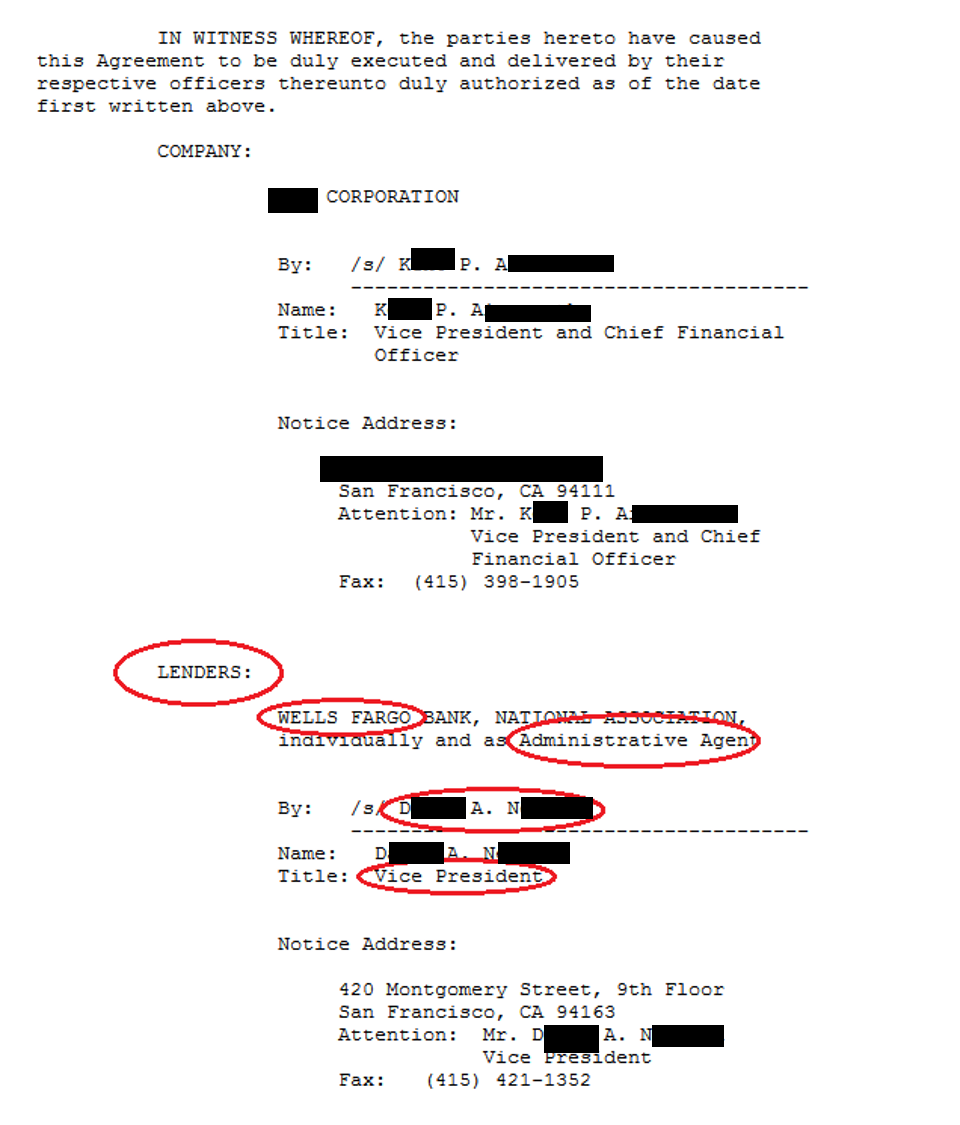
\includegraphics[angle=0,  scale=0.8]{figures/signature_well_formated.png}
\end{figure}

\clearpage \newpage

\begin{figure}[H]
	\caption{\textbf{Active bankers over time} \newline
		The figure shows the total number of active bankers in the sample (red line) and the cumulative number of bankers that switched and are still active (green line). Bankers are considered active for all years between the first and last deal they sign.}
	\label{fig:no_bankers}
	\centering
	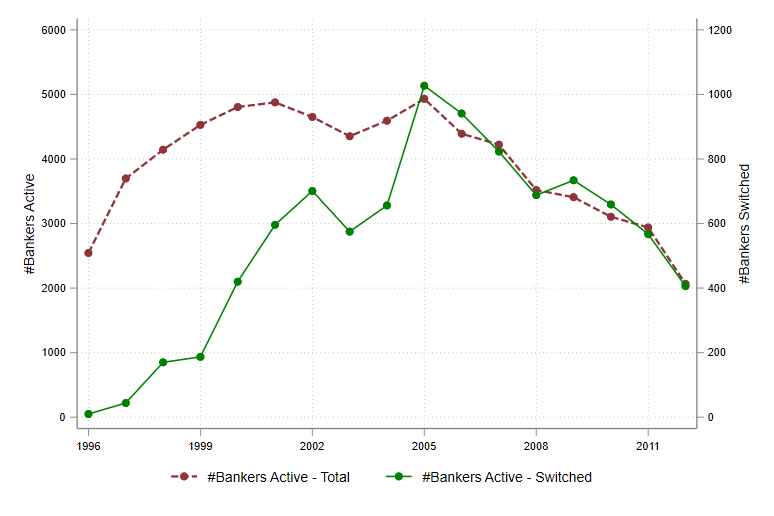
\includegraphics[angle=0,  scale=0.6]{figures/active_bankers_over_time.png}
\end{figure}
\clearpage \newpage

\begin{figure}[H]
	\caption{\textbf{Relationships acquired and initiations over time} \newline
		The figure shows the average yearly percentage of clients with whom a bank initiates a business relationship and for whom a personal relationship has been acquired. The x-axis show the number of years that elapsed since acquiring the relationship.
\textcolor{red}{CH: I am so sorry to keep pestering you about this graph but it still is not looking the way I have it in my head (and I am really stubborn :) ). This line should never go down. Right now, I understand the line some times goes down because some bankers are leaving the sample. I do not think that should happen if the data is constructed the way I think it is? Say we have some observations that took the value "initiation = 1, rel\_acq = 1". then the banker leaves the sample because she was inactive for 5 years (right? this is why the line only ever drops after 5 years?) But then initiation =1 and rel\_acq = 0? }	
}
	\label{fig:no_bankers}
	\centering
	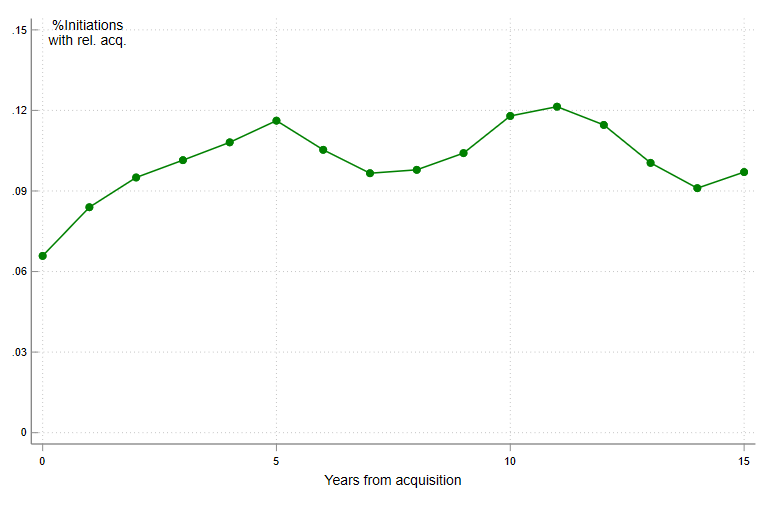
\includegraphics[angle=0,  scale=0.6]{figures/intiation_over_time.png}
\end{figure}



%
%%%%%%%%%%%%%%%%%%%%%%%%%%%%%%%%%%%%%%%%%%%%%%%%%%%%%%%
%Figure
%%%%%%%%%%%%%%%%%%%%%%%%%%%%%%%%%%%%%%%%%%%%%%%%%%%%%%%
%\begin{landscape}
%
%\begin{figure}[H]
%	\caption{Treatment dynamics (all deals) \newline
%		The figure presents the dynamics of treatment over time. Outcome variable is the log of dealsize across all three categories (loans, bonds, SEOs). Vertical bars represent 90\% confidence intervals for standard errors clustered at firm and lender. The year of treatment is the first year in which a banker appears on a loan for a new bank.} 
%	\label{fig:dynamics_full}
%	\centering
%	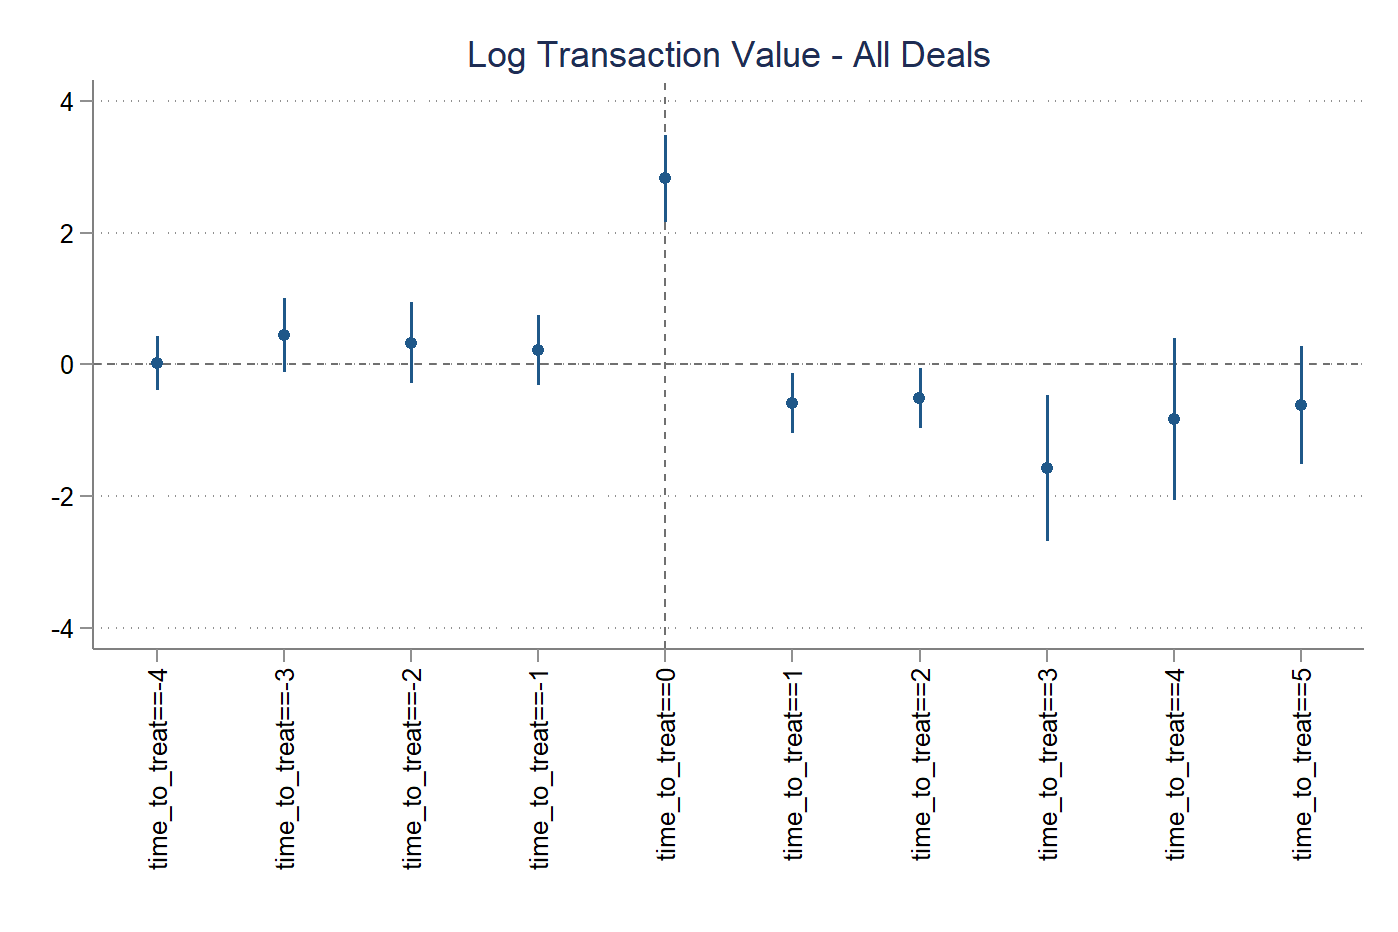
\includegraphics[angle=0,  scale=0.35]{figures/dynamics_logdealsize.png}
%\end{figure}
%\end{landscape}
%
%\clearpage \newpage
%%


%%%%%%%%%%%%%%%%%%%%%%%%%%%%%%%%%%%%%%%%%%%%%%%%%%%%%%%
%Figure
%%%%%%%%%%%%%%%%%%%%%%%%%%%%%%%%%%%%%%%%%%%%%%%%%%%%%%%
%
%\begin{figure}[H]
%	\caption{Treatment dynamics  (bonds only) \newline
%		The figure presents the dynamics of treatment over time. Outcome variable is the log of dealsize of new bonds issued. Vertical bars represent 90\% confidence intervals for standard errors clustered at firm and lender. The year of treatment is the first year in which a banker appears on a loan for a new bank.} 
%	\label{fig:dynamics_bonds}
%	\centering
%	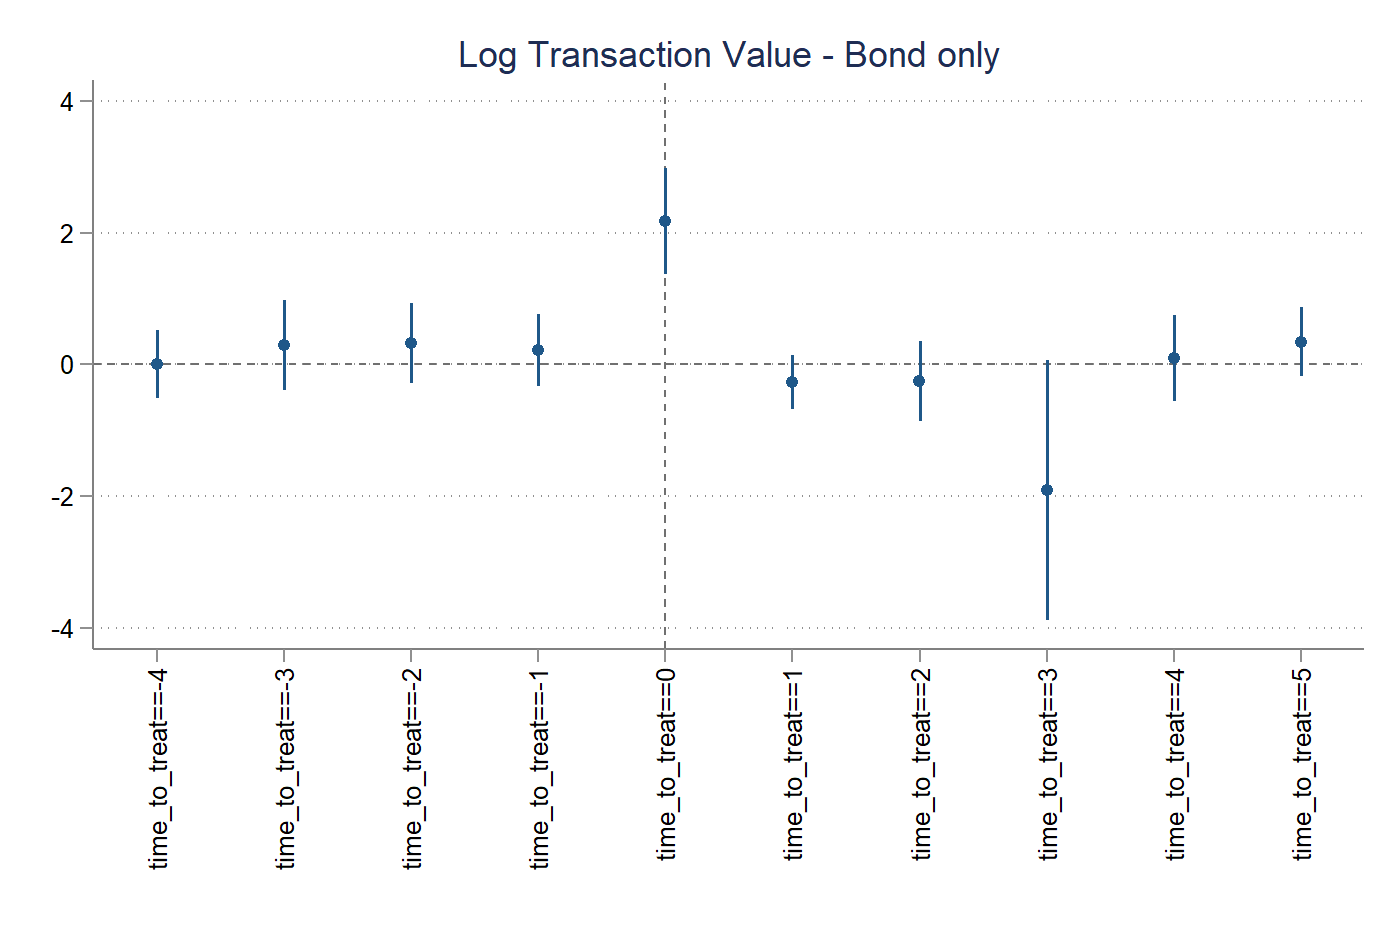
\includegraphics[angle=0,  scale=0.35]{figures/dynamics_logdealsize_bondonly.png}
%\end{figure}
%\end{landscape}
%
%\clearpage \newpage
%
%%%%%%%%%%%%%%%%%%%%%%%%%%%%%%%%%%%%%%%%%%%%%%%%%%%%%%%
%Figure
%%%%%%%%%%%%%%%%%%%%%%%%%%%%%%%%%%%%%%%%%%%%%%%%%%%%%%%
%
%
%\begin{figure}[H]
%	\caption{Treatment dynamics (SEO only) \newline
%		The figure presents the dynamics of treatment over time. Outcome variable is the log of dealsize of seasoned equity offerings. Vertical bars represent 90\% confidence intervals for standard errors clustered at firm and lender. The year of treatment is the first year in which a banker appears on a loan for a new bank.} 
%	\label{fig:dynamics_seo}
%	\centering
%	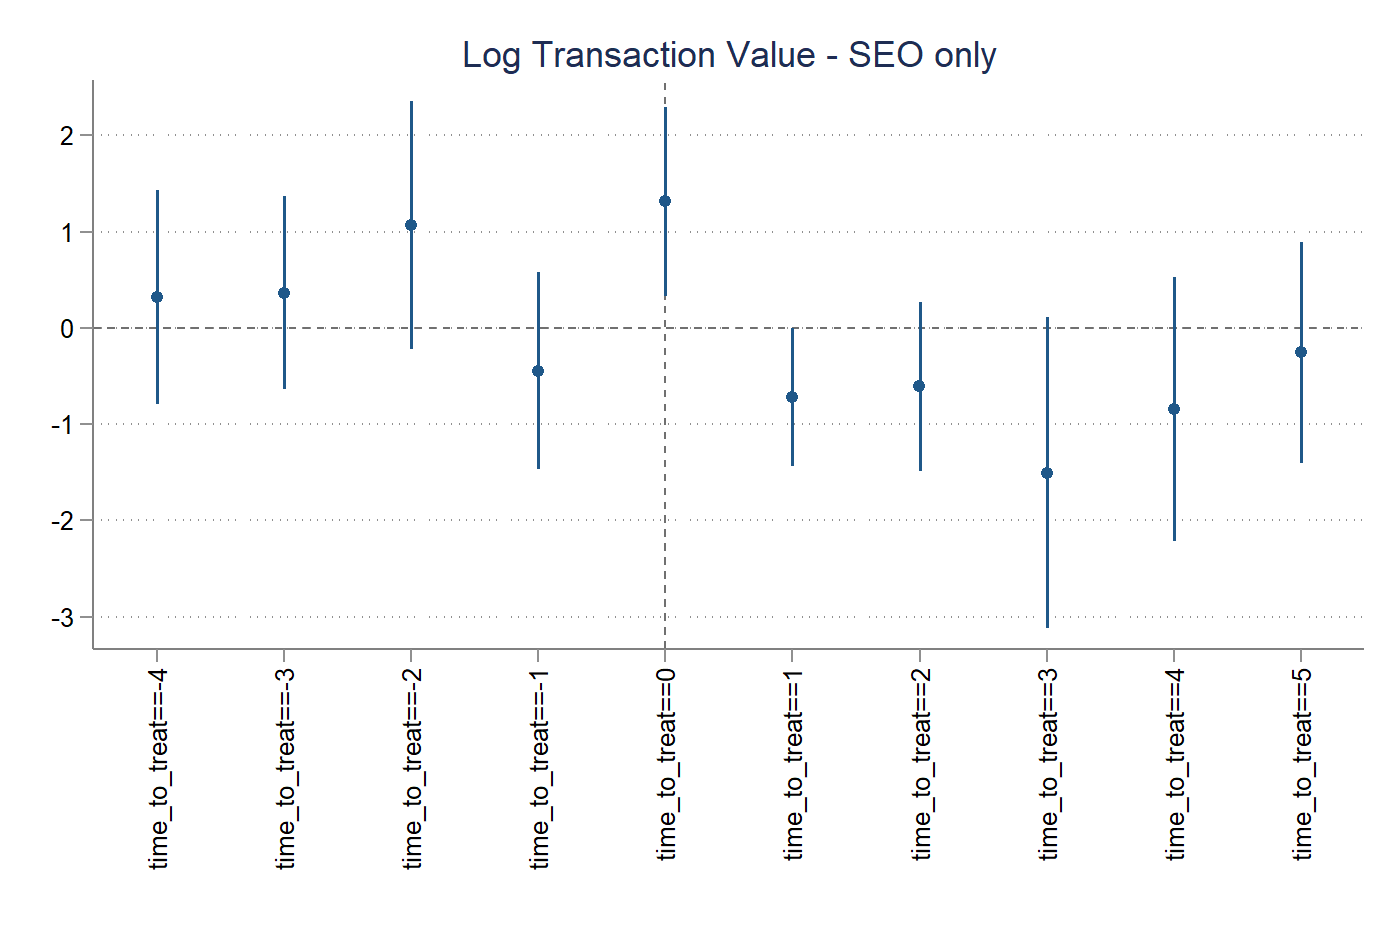
\includegraphics[angle=0,  scale=0.35]{figures/dynamics_logdealsize_seoonly.png}
%\end{figure}
%\end{landscape}
%
%\clearpage \newpage
%
%\begin{figure}[H]
%\captionsetup[subfigure]{justification=centering}
%	\centering
%	\caption{\textbf{Treatment dynamics - First deal and repeat business} \newline The figure presents the dynamics of treatment over time. Outcome variable in Panel A is the log of dealsize of the first deal (either syndicated loan, bond underwriting, or seasoned equity offering) in which a banker appears on a loan for a new bank. Panel B shows the total transaction value of repeated business done with a client (except for the first deal). Vertical bars represent 90\% confidence intervals for standard errors clustered at firm and lender. The year of treatment is the first year in which a banker appears on a loan for a new bank.} 
%	\label{fig:dynamics_first_repeated}
%	\begin{subfigure}[H]{\textwidth}
%		\centering
%		\caption*{\textbf{Panel A:} Log Transaction Value - First deal of old clients at new bank}
%		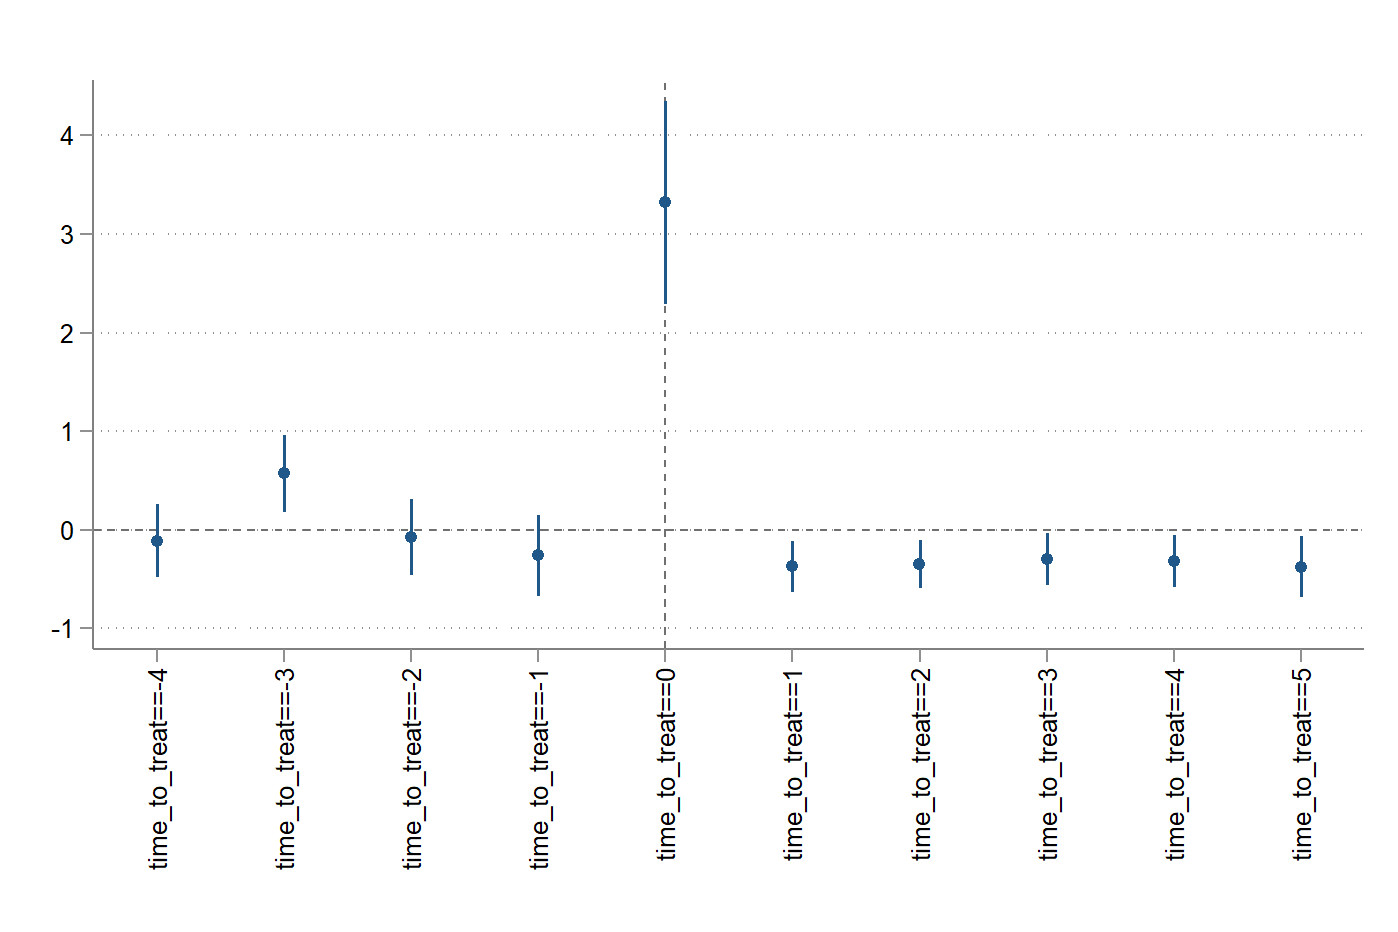
\includegraphics[angle=0,  scale=0.3]{figures/dynamics_logdealsize_firsttime.png}
%		\caption*{[Continued on the next page]}
%	\end{subfigure} \end{figure}
%
%\begin{figure}[H]
%\captionsetup[subfigure]{justification=centering}
%	{\small \centering [Continued from previous page] \\ ~ \newline}
%	\begin{subfigure}[H]{\textwidth}
%		\centering
%		\caption*{\textbf{Panel B:} Log Transaction Value - Repeat business with old clients at new bank}
%		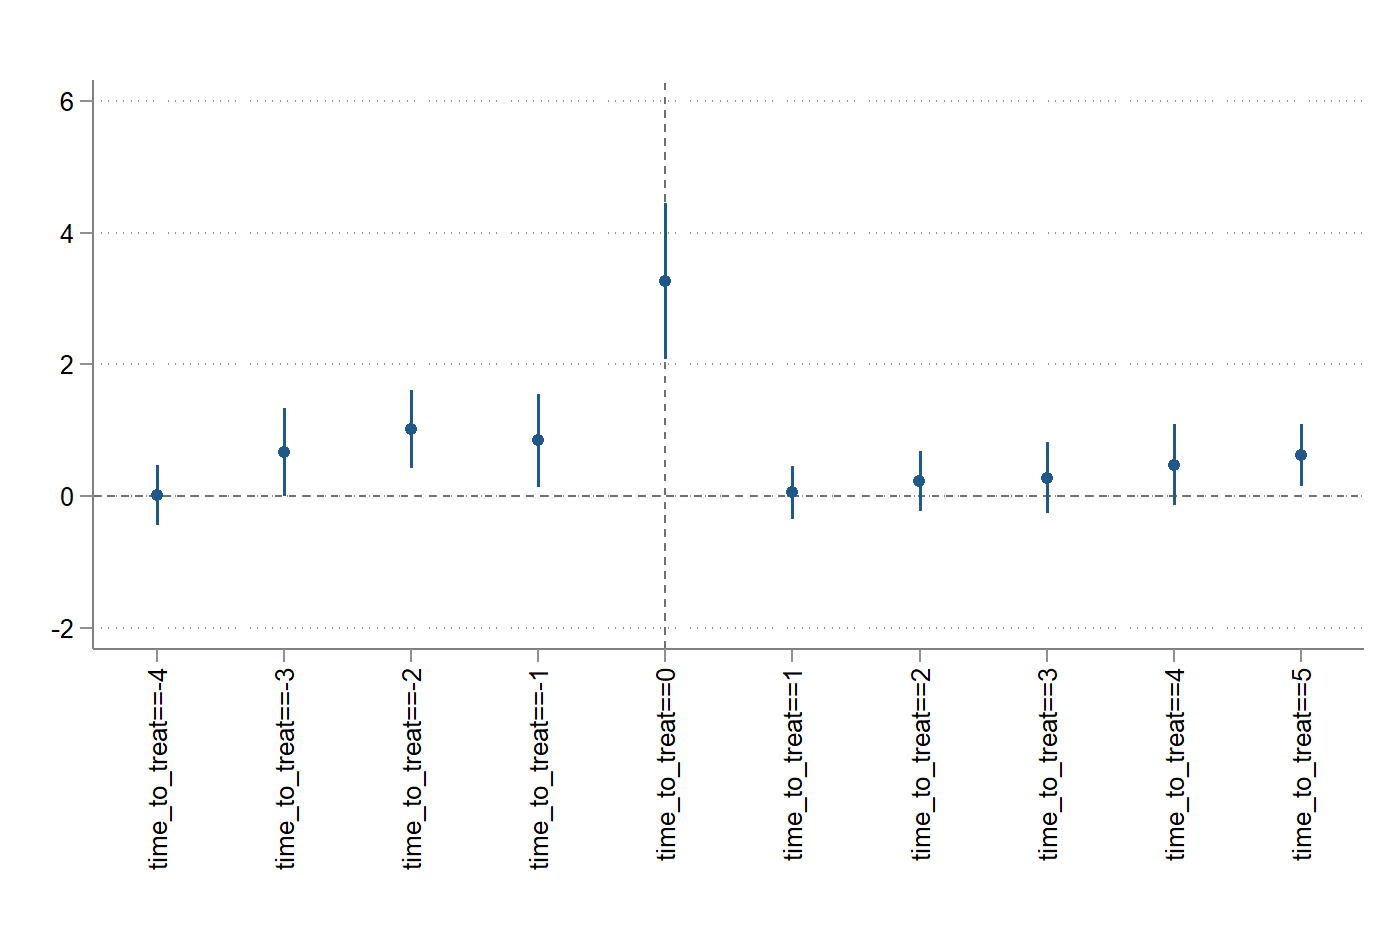
\includegraphics[angle=0,  scale=0.3]{figures/dynamics_logdealsize_repeat.png}
%	\end{subfigure}
%\end{figure}
%
%%%%%%%%%%%%%%%%%%%%%%%%%%%%%%%%%%%%%%%%%%%%%%%%%%%%%%%
%Figure
%%%%%%%%%%%%%%%%%%%%%%%%%%%%%%%%%%%%%%%%%%%%%%%%%%%%%%%
 \label{app:Figures}

\section*{Tables}
\label{app:Tables}



\singlespacing	


	
%	%%%%%%%%%%%%%%%%%%%%%%%%%%%%%%%%%%%%%%%%%%%%%%%%%%%%%%%%%%%%%%%%%%%%%%%%%%
%	Table 
%	SUMMARY STATS %%%%%%%%%%%%%%%%%%%%%%%%%%%%%%%%%%%%%%%%%%%%%%%%%%%%%%%%%%%%%%%%%%%%%%%%%%
\begin{table}[H] \begin{center} 
		\caption{\textbf{Summary statistics - Bankers’ personal relationships} \\ This table shows summary statistics of the sample variables relating to bankers' personal relationships. The sample in Panel A is at the banker-year level while in Panel B it is at the bank-year  level. All Panels cover the years from 1996 to 2013. The bankers' employment information and their client portfolio is retrieved from EDGAR. Firms' balance sheet information is from Compustat. Variables are defined as in Appendix Table \ref{tab:definitions}. }
		\label{tab:sumstat} 
	
	\begin{threeparttable} 
	\begin{tabular*}{\hsize} {@{\hskip\tabcolsep\extracolsep\fill}l*{7}{c}}
	 	\multicolumn{7}{l}{\textbf{Panel A}: Client portfolios of bankers} \\
		\toprule
		                    &           N&         p25&        mean&         p50&         p75&          sd\\
\midrule
Banker hired (\%)   &      66,774&        0.00&        1.57&        0.00&        0.00&       12.42\\
Banker female (\%)  &      58,663&        0.00&       18.91&        0.00&        0.00&       39.16\\
Tenure (yrs.)       &      66,774&        1.00&        3.72&        3.00&        5.00&        3.13\\
\#Clients - Total   &      66,774&        1.00&        3.07&        2.00&        3.00&        4.29\\
\#Clients - Small   &      66,774&        0.00&        0.08&        0.00&        0.00&        0.33\\
\#Clients - Large   &      66,774&        0.00&        1.50&        1.00&        2.00&        3.00\\
\#Clients - Single contact&      66,774&        0.00&        1.48&        1.00&        2.00&        2.37\\
\#Clients - Mult. contact&      66,774&        0.00&        1.58&        1.00&        2.00&        2.80\\
\#Deals - Total     &      66,774&        1.00&        4.14&        2.00&        5.00&        6.36\\
\#Deals - Small     &      66,774&        0.00&        0.11&        0.00&        0.00&        0.52\\
\#Deals - Large     &      66,774&        0.00&        1.97&        1.00&        2.00&        4.40\\
\#Deals - Mult. contact&      66,774&        0.00&        1.97&        1.00&        2.00&        4.25\\
\#Deals - Single contact&      66,774&        1.00&        2.51&        1.00&        3.00&        4.14\\
 	
		\bottomrule \\ ~ \\ 
	
	 	 \multicolumn{7}{l}{\textbf{Panel B}: Bank-level summary statistics} \\
			\toprule 
		                     &           N&         p25&        mean&         p50&         p75&          sd\\
\midrule
\#Bankers employed  &      12,959&        1.00&       16.00&        3.00&        9.00&       49.55\\
Mean deals per banker-yr&      12,964&        1.00&        1.46&        1.00&        2.00&        2.03\\
\#Clients - Total   &      12,937&        2.00&       28.91&        6.00&       18.00&       82.48\\
\#Clients - Small   &      12,964&        0.00&        0.32&        0.00&        0.00&        0.79\\
\#Clients - Large   &      12,964&        0.50&        2.73&        1.00&        3.00&        4.47\\
\#Clients - Mult. bankers&      12,964&        0.00&        0.25&        0.00&        0.00&        0.43\\
Discrimination lawsuit&      12,964&        0.00&        0.03&        0.00&        0.00&        0.16\\
 
		 		\bottomrule
	\end{tabular*} 	\end{threeparttable}  \end{center} \end{table}
\newpage

\begin{table}[H] \begin{center} 
		\caption{\textbf{Summary statistics - Banks’ client portfolio} \\ This table shows summary statistics of the sample variables relating to the banks' client portfolio The sample is at the bank-borrower-year level and covers the years from 1996 to 2013. Panel A shows all bank-firm pairs, while Panel B shows deal volume conditional on signing at least one deal for a given bank-borrower-year. Panel C shows summary statistics at the firm-year level. The bankers' employment information and their client portfolio is retrieved from EDGAR. Bond ans SEO underwriting as well as M\&A advisory deals are retrieved from CapitalIQ. Syndicated loans are from Dealscan. Balance sheet information is from Compustat. Variables are defined as in Appendix Table \ref{tab:definitions}. }
		\label{tab:sumstat_bank} 
	\begin{threeparttable}  
		\begin{tabular*}{\hsize} {@{\hskip\tabcolsep\extracolsep\fill}l*{7}{c}}
		 \multicolumn{7}{l}{\textbf{Panel A}: All bank-firm pairs} \\ \toprule 
		                     &           N&         p25&        mean&         p50&         p75&          sd\\
\midrule
Rel\_acq (\%)       &     972,090&        0.00&        2.93&        0.00&        0.00&       16.86\\
Rel\_acq\(^{5yr}\) (\%)&     958,299&        0.00&        1.53&        0.00&        0.00&       12.28\\
Rel\_acq\(^{abs}\) (\%)&     946,214&        0.00&        0.27&        0.00&        0.00&        5.23\\
Rel\_acq\_nofirst (\%)&     969,584&        0.00&        2.68&        0.00&        0.00&       16.14\\
Rel\_acq\_nofirst\(^{5yr}\) (\%)&     955,796&        0.00&        1.27&        0.00&        0.00&       11.22\\
Rel\_acq\_nofirst\(^{abs}\) (\%)&     946,311&        0.00&        0.28&        0.00&        0.00&        5.33\\
Initiation (\%)     &     972,090&        0.00&        5.20&        0.00&        0.00&       22.19\\
 
		 \bottomrule \\ ~ \\ 
	
	 	 \multicolumn{7}{l}{\textbf{Panel B}: All bank-firm pairs, conditional on signing at least one deal} \\
			\toprule 
			                     &           N&         p25&        mean&         p50&         p75&          sd\\
\midrule
Volume - All deals  &      89,066&      100.00&      827.93&      276.45&      718.11&    2,543.72\\
Volume - Synd. Loans&      89,066&        0.00&      417.48&       25.00&      300.00&    1,571.22\\
Volume - Bonds      &      89,066&        0.00&      279.48&        0.00&      185.32&    1,215.99\\
Volume - SEOs       &      89,066&        0.00&       56.23&        0.00&        0.00&      459.01\\
Volume - M\&As      &      89,066&        0.00&       74.74&        0.00&        0.00&    1,281.47\\
\#Deals - Total     &      89,066&        1.00&        1.74&        1.00&        1.00&       17.43\\
\#Delas - Synd. loans&      89,066&        0.00&        0.64&        1.00&        1.00&        0.75\\
\#Delas - Bonds     &      89,066&        0.00&        0.81&        0.00&        1.00&       17.45\\
\#Delas - SEOs      &      89,066&        0.00&        0.17&        0.00&        0.00&        0.45\\
\#Delas - M\&A      &      89,066&        0.00&        0.04&        0.00&        0.00&        0.21\\

				\bottomrule \\ ~ \\

		\multicolumn{7}{l}{\textbf{Panel C}: Firm-level variables} \\
	\toprule 
 		                     &           N&         p25&        mean&         p50&         p75&          sd\\
\midrule
Total Assets        &      78,401&      179.19&    6,922.45&      731.36&    3,106.57&   26,354.11\\
Leverage            &      77,547&        0.38&        0.57&        0.56&        0.73&        0.29\\
EBITDA              &      74,450&        5.20&      226.95&       32.97&      133.74&      771.83\\
Profitability       &      72,453&        0.02&        0.05&        0.04&        0.11&        0.15\\
Intangibles to Assets&      64,579&        0.00&        0.14&        0.05&        0.22&        0.19\\
 
 		 	\bottomrule 
		 % \\~\\ \multicolumn{7}{c}{[Continued on the next page]} 
	\end{tabular*} 	\end{threeparttable}  \end{center} \end{table}

\clearpage \newpage

% \newpage
% \begin{table}[H] \begin{center} \begin{threeparttable} 
% 		\begin{tabular*}{\hsize} {@{\hskip\tabcolsep\extracolsep\fill}l*{7}{c}}
% 		 	 \multicolumn{7}{c}{[Continued from previous page]} \\ \\
% 			 	 \multicolumn{7}{l}{\textbf{Panel C}: Firm-level variables} \\
% 			\toprule 
% 		                     &           N&         p25&        mean&         p50&         p75&          sd\\
\midrule
Total Assets        &      78,401&      179.19&    6,922.45&      731.36&    3,106.57&   26,354.11\\
Leverage            &      77,547&        0.38&        0.57&        0.56&        0.73&        0.29\\
EBITDA              &      74,450&        5.20&      226.95&       32.97&      133.74&      771.83\\
Profitability       &      72,453&        0.02&        0.05&        0.04&        0.11&        0.15\\
Intangibles to Assets&      64,579&        0.00&        0.14&        0.05&        0.22&        0.19\\
 
% 		 	\bottomrule \\
% 		 	\multicolumn{7}{l}{\textbf{Panel D}: Bank-level variables} \\
% 		 	\bottomrule \\
% 		                    &           N&         p25&        mean&         p50&         p75&          sd\\
\midrule
Log Assets          &     202,998&       12.62&       13.28&       13.48&       14.24&        1.17\\
Leverage            &     202,993&        0.91&        0.93&        0.93&        0.95&        0.03\\
EBITDA              &     181,712&    1,668.00&    6,004.43&    4,252.00&    8,714.00&    5,896.76\\
Profitability       &     176,502&        0.00&        0.01&        0.01&        0.01&        0.01\\
Intangibles to Assets&     177,299&        0.01&        0.02&        0.02&        0.03&        0.02\\
 
% 		 	\multicolumn{7}{l}{\textbf{Panel E}: Variation within groups} \\
% \bottomrule \\
%     & \multicolumn{1}{c}{} & \multicolumn{2}{c}{Overall} & \multicolumn{1}{c}{SD within} & \multicolumn{1}{c}{SD within} & \multicolumn{1}{c}{SD within}\\
    
    & \multicolumn{1}{c}{$N$} & \multicolumn{2}{c}{SD} &\multicolumn{1}{c}{firm-year}&\multicolumn{1}{c}{bank-firm} & \multicolumn{1}{c}{bank-year}\\
\hline
1(downgrade) &   				20,725 &  \multicolumn{2}{c}{16.88} &   16.61 &    15.91 &   16.74\\
Cost~of~downgrade~(bps) &   	20,725 &  \multicolumn{2}{c}{11.89} &   10.66 &     8.81 &   11.71\\
Time to downgrade (quarters) &   2,868 &  \multicolumn{2}{c}{4.50} &     4.42 &     3.71 &    4.25\\ 
% 		 	\bottomrule \\
% 		 \end{tabular*}
% 	\end{threeparttable} \end{center}
% \end{table}

%%%%%%%%%%%%%%%%%%%%%%%%%%%%%%%%%%%%%%%%%%%%%%%%%%%%%%%%%
%	WHY DO BANKERS SWITCH? %%%%%%%%%%%%%%%%%%%%%%%%%%%%%%%%%%%%%%%%%%%%%%%%%%%%%%%%%% 

\begin{table}[H] \begin{center} 
	\caption{\textbf{Bankers' switching and size of client portfolio} \\ This table shows regressions of an indicator value (in \%) for the first year a banker appears at a new bank on the lagged client portfolio characteristics of the banker. In Panel A these are the number of clients and in Panel B the number of deals  that the banker signs with her client portfolio at the bank. Columns (3) and (4) show the portfolio characteristics by clients' size. Columns (5) and (6) explore the trade off between the quantity and quality of the client portfolio by treating the single contact and multiple contact clients separately. The sample covers all banker-years pairs between 1996 and 2013. Variables are defined as in Appendix Table~\ref{tab:definitions}. t-statistics, based on robust standard errors clustered two dimensionally at lender and bank level, are reported in parentheses. ***, **, and * indicate that the parameter estimate is significantly different from zero at the 1\%, 5\%, and 10\% level, respectively.} 
		\label{tab:banker_clientno} 
	\begin{threeparttable} 
		\begin{tabular*}{\hsize} {@{\hskip\tabcolsep\extracolsep\fill}l*{7}{c}}
		 \multicolumn{7}{l}{\textbf{Panel A}: Number of clients} \\ \toprule 

		 			Dep. variable:                 &\multicolumn{6}{c}{Banker hired (\%)}                                        \\\cmidrule(lr){2-7}
                &\multicolumn{1}{c}{(1)}   &\multicolumn{1}{c}{(2)}   &\multicolumn{1}{c}{(3)}   &\multicolumn{1}{c}{(4)}   &\multicolumn{1}{c}{(5)}   &\multicolumn{1}{c}{(6)}   \\
\midrule
\#Clients - Total\(_{t-1}\)&     0.21***&     0.15***&            &            &            &            \\
                &   (4.42)   &   (3.87)   &            &            &            &            \\
 
\#Clients - Small\(_{t-1}\)&            &            &     0.63** &     0.34   &            &            \\
                &            &            &   (2.02)   &   (1.07)   &            &            \\
 
\#Clients - Large\(_{t-1}\)&            &            &     0.25***&     0.17***&            &            \\
                &            &            &   (4.04)   &   (3.43)   &            &            \\
 
\#Clients - Single contact\(_{t-1}\)&            &            &            &            &     0.46***&     0.58***\\
                &            &            &            &            &   (3.67)   &   (4.14)   \\
 
\#Clients - Mult. contact\(_{t-1}\)&            &            &            &            &     0.02   &    -0.14** \\
                &            &            &            &            &   (0.25)   &  (-2.10)   \\
\midrule
Observations    &   46,075   &   39,992   &   46,075   &   39,992   &   46,075   &   39,992   \\
R-squared       &     0.11   &     0.21   &     0.11   &     0.21   &     0.11   &     0.22   \\
Bank and Year FE&      Yes   &       No   &      Yes   &       No   &      Yes   &       No   \\
Bank $\times$ Year FE&       No   &      Yes   &       No   &      Yes   &       No   &      Yes   \\
  
		 		\bottomrule 
		 \\ \multicolumn{7}{c}{[Continued on the next page]} 
\end{tabular*} 	\end{threeparttable}  \end{center} \end{table}

%%%%%%%%%%%%%%%%%%% PANEL B %%%%%%%%%%%%%%%%%
\begin{table}[H] \begin{center} \begin{threeparttable} 
 		\begin{tabular*}{\hsize} {@{\hskip\tabcolsep\extracolsep\fill}l*{7}{c}}
 		 	 \multicolumn{7}{c}{[Continued from previous page]} \\ \\
	 	 \multicolumn{7}{l}{\textbf{Panel B}: Number of deals} \\
			\toprule 

			Dep. variable:                &\multicolumn{6}{c}{Banker hired (\%)}                                        \\\cmidrule(lr){2-7}
                &\multicolumn{1}{c}{(1)}   &\multicolumn{1}{c}{(2)}   &\multicolumn{1}{c}{(3)}   &\multicolumn{1}{c}{(4)}   &\multicolumn{1}{c}{(5)}   &\multicolumn{1}{c}{(6)}   \\
\midrule
Total \#Deals\(_{t-1}\)&     0.14***&     0.10***&            &            &            &            \\
                &   (4.66)   &   (4.05)   &            &            &            &            \\
 
\#Deals - Small\(_{t-1}\)&            &            &     0.38** &     0.18   &            &            \\
                &            &            &   (2.02)   &   (1.10)   &            &            \\
 
\#Deals - Large\(_{t-1}\)&            &            &     0.16***&     0.11***&            &            \\
                &            &            &   (3.99)   &   (3.35)   &            &            \\
 
\#Deals - Single contact\(_{t-1}\)&            &            &            &            &     0.08** &     0.11***\\
                &            &            &            &            &   (2.19)   &   (2.79)   \\
 
\#Deals - Mult. contact\(_{t-1}\)&            &            &            &            &     0.06   &    -0.02   \\
                &            &            &            &            &   (1.29)   &  (-0.52)   \\
\midrule
Observations    &   46,075   &   39,992   &   46,075   &   39,992   &   46,075   &   39,992   \\
R-squared       &     0.11   &     0.21   &     0.11   &     0.21   &     0.11   &     0.21   \\
Bank and Year FE&      Yes   &       No   &      Yes   &       No   &      Yes   &       No   \\
Bank $\times$ Year FE&       No   &      Yes   &       No   &      Yes   &       No   &      Yes   \\

					\bottomrule 
	\end{tabular*} 	 \end{threeparttable}   \end{center} \end{table}
\clearpage \newpage


% \begin{table}[H] \begin{center} 
% \caption{\textbf{Switching bankers and deal volume at old bank} \\ This table shows regressions of an indicator value (in \%) for the pre-switch period on the total volume of deals that the banker's portfolio clients had with a bank during a year. Columns 3, 4, and 5 show the volume separately by deal types. The sample covers all banker-years pairs between 1996 and 2013 for the banks that could be matched with Compustat. Variables are defined as in Appendix Table~\ref{tab:definitions}. t-statistics, based on robust standard errors clustered two dimensionally at lender and banker level, are reported in parentheses. ***, **, and * indicate that the parameter estimate is significantly different from zero at the 1\%, 5\%, and 10\% level, respectively. } 
% 	\label{tab:banker_clientno} 
% \begin{threeparttable} 
% 			{
\def\sym#1{\ifmmode^{#1}\else\(^{#1}\)\fi}
\begin{tabular*}{\hsize}{@{\hskip\tabcolsep\extracolsep\fill}l*{5}{c}}
\toprule
                &\multicolumn{5}{c}{Pre-Switch Indicator (\%)}                   \\\cmidrule(lr){2-6}
                &\multicolumn{1}{c}{(1)}   &\multicolumn{1}{c}{(2)}   &\multicolumn{1}{c}{(3)}   &\multicolumn{1}{c}{(4)}   &\multicolumn{1}{c}{(5)}   \\
\midrule
Log Deal Volume &     0.58***&     0.63***&            &            &            \\
                &   (2.98)   &   (3.66)   &            &            &            \\
 
Log Syndicated Loans&            &            &     0.40   &            &            \\
                &            &            &   (1.57)   &            &            \\
 
Log Bonds       &            &            &            &     0.32*  &            \\
                &            &            &            &   (1.83)   &            \\
 
Log SEOs        &            &            &            &            &     0.81   \\
                &            &            &            &            &   (1.48)   \\
\midrule
Observations    &   14,126   &   13,897   &   13,897   &   13,897   &   13,897   \\
R-squared       &     0.07   &     0.14   &     0.14   &     0.14   &     0.14   \\
\midrule Year FE &      Yes   &       No   &       No   &       No   &       No   \\
Bank FE         &      Yes   &       No   &       No   &       No   &       No   \\
Bank-Year FE    &       No   &      Yes   &      Yes   &      Yes   &      Yes   \\
\bottomrule
\end{tabular*}
}
  
% \end{threeparttable}   \end{center} \end{table}


%	%%%%%%%%%%%%%%%%%%%%%%%%%%%%%%%%%%%%%%%%%%%%%%%%%%%%%%%%%%%%%%%%%%%%%%%%%%
%	Table INITIATION
%	%%%%%%%%%%%%%%%%%%%%%%%%%%%%%%%%%%%%%%%%%%%%%%%%%%%%%%%%%%%%%%%%%%%%%%%%%%
\begin{table}[H] \begin{center} 
		\caption{\textbf{Initiation} \\ This table shows regressions of an indicator for a new bank-borrower relationships on an indicator for  personal relationship acquired, which identifies deals with the old clients of bankers that switch employers. In columns (1) to (4), the indicator variable takes the value of one for all years after the banker switches. In (5) and (6) it is set to missing after 5 and 1 year respectively. The dependent variable is an indicator for bank-borrower relationships that are new or for whom the bank had no interaction in the past 5 years. The sample is at the bank-borrower-year level and spans from 1996 to 2013. Bond and SEO underwriting as well as M\&A advisory deals are retrieved from CapitalIQ. Syndicated loans are from Dealscan. Variables are defined as in Appendix Table \ref{tab:definitions}. t-statistics, based on robust standard errors clustered two dimensionally at firm and lender level, are reported in parentheses. ***, **, and * indicate that the parameter estimate is significantly different from zero at the 1\%, 5\%, and 10\% level, respectively. } %  ...SAMPLE DESCRIPTION. MAIN OUTCOME. CLUSTERS. STARS 
		\label{tab:init} 
	\begin{threeparttable} 
		%% PANEL A -> INITIATION
		\begin{tabular*}{\hsize}{@{\hskip\tabcolsep\extracolsep\fill}l*{6}{c}} \def\sym#1{\ifmmode^{#1}\else\(^{#1}\)\fi} 
		\\ \toprule
				                Dep. variable: &\multicolumn{6}{c}{Initiation}                                               \\\cmidrule(lr){2-7}
                &\multicolumn{1}{c}{(1)}   &\multicolumn{1}{c}{(2)}   &\multicolumn{1}{c}{(3)}   &\multicolumn{1}{c}{(4)}   &\multicolumn{1}{c}{(5)}   &\multicolumn{1}{c}{(6)}   \\
\midrule
Rel\_acq        &     0.07** &     0.09** &     0.13***&     0.14***&            &            \\
                &   (2.37)   &   (2.38)   &   (3.58)   &   (3.80)   &            &            \\
 
Rel\_acq\(^{5yr}\)&            &            &            &            &     0.12***&            \\
                &            &            &            &            &   (3.54)   &            \\
 
Rel\_acq\(^{abs}\)&            &            &            &            &            &     0.07***\\
                &            &            &            &            &            &   (3.34)   \\
\midrule
Observations    &  861,444   &  861,444   &  861,444   &  861,444   &  847,102   &  834,461   \\
R-squared       &     0.03   &     0.08   &     0.10   &     0.42   &     0.41   &     0.41   \\
\midrule Year FE &      Yes   &      Yes   &      Yes   &       No   &       No   &       No   \\
Firm FE         &      Yes   &       No   &       No   &       No   &       No   &       No   \\
Bank FE         &      Yes   &       No   &       No   &       No   &       No   &       No   \\
Firm-Bank FE    &       No   &      Yes   &      Yes   &      Yes   &      Yes   &      Yes   \\
Bank-Year FE    &       No   &       No   &      Yes   &      Yes   &      Yes   &      Yes   \\
Firm-Year FE    &       No   &       No   &       No   &      Yes   &      Yes   &      Yes   \\

		\bottomrule \end{tabular*}
\end{threeparttable}   \end{center} \end{table}
\clearpage \newpage


%	%%%%%%%%%%%%%%%%%%%%%%%%%%%%%%%%%%%%%%%%%%%%%%%%%%%%%%%%%%%%%%%%%%%%%%%%%%
%	Table INITIATION-cross section
%	%%%%%%%%%%%%%%%%%%%%%%%%%%%%%%%%%%%%%%%%%%%%%%%%%%%%%%%%%%%%%%%%%%%%%%%%%%
\begin{table}[H] \begin{center} 
		\caption{\textbf{Initiation - Opaque clients} \\ This table shows regressions of XXX Variables are defined as in Appendix Table \ref{tab:definitions}. t-statistics, based on robust standard errors clustered at firm and lender level, are reported in parentheses. ***, **, and * indicate that the parameter estimate is significantly different from zero at the 1\%, 5\%, and 10\% level, respectively. } %  ...SAMPLE DESCRIPTION. MAIN OUTCOME. CLUSTERS. STARS 
		\label{tab:init_cross} 
		\begin{threeparttable}  \def\sym#1{\ifmmode^{#1}\else\(^{#1}\)\fi}
			\begin{tabular*}{.8\hsize}{@{\hskip\tabcolsep\extracolsep\fill}l*{3}{c}} \toprule
				                Dep. variable: &\multicolumn{3}{c}{Initiation}        \\\cmidrule(lr){2-4}
                &\multicolumn{1}{c}{(1)}   &\multicolumn{1}{c}{(2)}   &\multicolumn{1}{c}{(3)}   \\
\midrule
Rel\_acq $\times$ Junk&     0.16***&            &            \\
                &   (3.82)   &            &            \\
 
Junk&     0.01*  &            &            \\
                &   (1.85)   &            &            \\
 
Rel\_acq &     0.22***&            &            \\
                &   (3.77)   &            &            \\
 
Rel\_acq $\times$ Hi Intang&            &     0.19***&            \\
                &            &   (3.63)   &            \\
 
Hi Intang&            &     0.02***&            \\
                &            &   (3.91)   &            \\
 
Rel\_acq&            &     0.16***&            \\
                &            &   (3.43)   &            \\
 
Rel\_acq $\times$ Small&            &            &     0.07***\\
                &            &            &   (3.76)   \\
 
Small&            &            &    -0.01***\\
                &            &            &  (-2.95)   \\
 
Rel\_acq&            &            &     0.15***\\
                &            &            &   (3.49)   \\
\midrule
Observations    &  203,874   &  355,856   &  434,134   \\
R-squared       &     0.22   &     0.16   &     0.15   \\
\midrule Year FE &      Yes   &      Yes   &      Yes   \\
Firm-Bank FE    &      Yes   &      Yes   &      Yes   \\
Bank-Year FE    &      Yes   &      Yes   &      Yes   \\
 
				\bottomrule \end{tabular*}
\end{threeparttable}   \end{center} \end{table}
\clearpage \newpage

%	%%%%%%%%%%%%%%%%%%%%%%%%%%%%%%%%%%%%%%%%%%%%%%%%%%%%%%%%%%%%%%%%%%%%%%%%%%
%	Table  log deal size any
%	%%%%%%%%%%%%%%%%%%%%%%%%%%%%%%%%%%%%%%%%%%%%%%%%%%%%%%%%%%%%%%%%%%%%%%%%%%
\begin{table}[H] \begin{center} 
	\caption{\textbf{Total deal volume} \\ This table shows regressions of the logarithm of total deal volume on an indicator for personal relationship acquired, which identifies deals with the old clients of bankers that switch employers. The indicator variable takes the value of one for all years after the banker switches in columns (1) to (4) while in (5) and (6) it is set to missing after 5 and 1 year respectively. Panel B adds the interaction terms with an indicator for bank-borrower relationships that are new or for whom the bank had no interaction in the past 5 years. Firms for which a relationship is acquired but never close a deal with the bank are dropped. The sample is at the bank-borrower-year level and spans from 1996 to 2013. Bond and SEO underwriting as well as M\&A advisory deals are retrieved from CapitalIQ. Syndicated loans are from Dealscan. Variables are defined as in Appendix Table \ref{tab:definitions}. t-statistics, based on robust standard errors clustered two dimensionally at firm and lender level, are reported in parentheses. ***, **, and * indicate that the parameter estimate is significantly different from zero at the 1\%, 5\%, and 10\% level, respectively. }  
		\label{tab:main_dealsize} 
	\begin{threeparttable} 
	%%%%%%% PANEL A
	\begin{tabular*}{\hsize}{@{\hskip\tabcolsep\extracolsep\fill}l*{6}{c}}
	\multicolumn{6}{l}{\textbf{Panel A}: Relationship acquired} \\	\toprule  
	\def\sym#1{\ifmmode^{#1}\else\(^{#1}\)\fi}

				                Dep. variable: &\multicolumn{6}{c}{Log Deal Volume}                                          \\\cmidrule(lr){2-7}
                &\multicolumn{1}{c}{(1)}   &\multicolumn{1}{c}{(2)}   &\multicolumn{1}{c}{(3)}   &\multicolumn{1}{c}{(4)}   &\multicolumn{1}{c}{(5)}   &\multicolumn{1}{c}{(6)}   \\
\midrule
Rel\_acq        &     0.66***&     0.72***&     0.62***&     0.35***&            &            \\
                &   (6.78)   &   (3.79)   &   (4.58)   &   (3.85)   &            &            \\
 
Rel\_acq\(^{5yr}\)&            &            &            &            &     0.37***&            \\
                &            &            &            &            &   (3.82)   &            \\
 
Rel\_acq\(^{abs}\)&            &            &            &            &            &     2.34***\\
                &            &            &            &            &            &   (6.20)   \\
\midrule
Observations    &  809,173   &  809,173   &  809,173   &  809,173   &  807,720   &  806,190   \\
R-squared       &     0.07   &     0.14   &     0.16   &     0.51   &     0.51   &     0.51   \\
\midrule Year FE &      Yes   &      Yes   &      Yes   &       No   &       No   &       No   \\
Firm FE         &      Yes   &       No   &       No   &       No   &       No   &       No   \\
Firm-Bank FE    &       No   &      Yes   &      Yes   &      Yes   &      Yes   &      Yes   \\
Bank-Year FE    &       No   &       No   &      Yes   &      Yes   &      Yes   &      Yes   \\
Firm-Year FE    &       No   &       No   &       No   &      Yes   &      Yes   &      Yes   \\
  
	\bottomrule \\  \multicolumn{6}{c}{[Continued on the next page]}  \end{tabular*}
	\end{threeparttable}   \end{center} \end{table}
\clearpage \newpage

\begin{table}[H] \begin{center} \begin{threeparttable} 
	%%%%%%% PANEL B -> CIQ BONDS
	\begin{tabular*}{\hsize}{@{\hskip\tabcolsep\extracolsep\fill}l*{6}{c}}
			 \multicolumn{6}{c}{[Continued from previous page]} \\ \\
			 \multicolumn{6}{l}{\textbf{Panel B}: Interaction with initiation} \\
			\toprule  \def\sym#1{\ifmmode^{#1}\else\(^{#1}\)\fi}

		                Dep. variable: &\multicolumn{6}{c}{Log Deal Volume}                                          \\\cmidrule(lr){2-7}
                &\multicolumn{1}{c}{(1)}   &\multicolumn{1}{c}{(2)}   &\multicolumn{1}{c}{(3)}   &\multicolumn{1}{c}{(4)}   &\multicolumn{1}{c}{(5)}   &\multicolumn{1}{c}{(6)}   \\
\midrule
Rel\_acq \(\times\) Initiation&     1.64***&     1.58***&     1.53***&     1.21***&            &            \\
                &  (14.37)   &   (8.44)   &  (10.11)   &  (11.11)   &            &            \\
 
Rel\_acq        &    -0.29***&    -0.43***&    -0.45***&    -0.42***&            &            \\
                &  (-4.91)   &  (-2.69)   &  (-3.14)   &  (-3.96)   &            &            \\
 
Initiation      &     4.91***&     4.84***&     4.81***&     4.55***&            &            \\
                &  (64.61)   &  (63.95)   &  (61.92)   &  (95.03)   &            &            \\
 
Rel\_acq\(^{5yr}\) $\times$ Initiation&            &            &            &            &     1.37***&            \\
                &            &            &            &            &  (11.22)   &            \\
 
Rel\_acq\(^{5yr}\)&            &            &            &            &    -0.38***&            \\
                &            &            &            &            &  (-3.59)   &            \\
 
Initiation~     &            &            &            &            &     4.55***&            \\
                &            &            &            &            &  (96.22)   &            \\
 
Rel\_acq\(^{abs}\) $\times$ Initiation&            &            &            &            &            &     3.52***\\
                &            &            &            &            &            &   (8.96)   \\
 
Rel\_acq\(^{abs}\)&            &            &            &            &            &     0.88** \\
                &            &            &            &            &            &   (2.01)   \\
 
Initiation~~    &            &            &            &            &            &     4.56***\\
                &            &            &            &            &            &  (98.81)   \\
\midrule
Observations    &  921,504   &  921,504   &  921,504   &  809,173   &  807,720   &  806,190   \\
R-squared       &     0.53   &     0.57   &     0.58   &     0.73   &     0.73   &     0.74   \\
\midrule Year FE &      Yes   &      Yes   &      Yes   &       No   &       No   &       No   \\
Firm FE         &      Yes   &       No   &       No   &       No   &       No   &       No   \\
Firm-Bank FE    &       No   &      Yes   &      Yes   &      Yes   &      Yes   &      Yes   \\
Bank-Year FE    &       No   &       No   &      Yes   &      Yes   &      Yes   &      Yes   \\
Firm-Year FE    &       No   &       No   &       No   &      Yes   &      Yes   &      Yes   \\
  
		\bottomrule \end{tabular*}
	\end{threeparttable}   \end{center} \end{table}
\clearpage \newpage

%	\caption{\textbf{Total deal volume - Interaction with initiation} \\ This table shows regressions of the logarithm of total deal volume on an indicator for  personal relationship acquired, which identifies deals with the old clients of bankers that switch employers. The indicator variable takes the value of one for all years after the banker switches. Initiation identifies new bank-borrower relationships as well as clients with whom the bank had no interaction in the past 5 years. Firms for which a relationship is acquired but never close a deal with the bank are dropped. The sample is at the bank-borrower-year level and spans from 1996 to 2013. Bond and SEO underwriting as well as M\&A advisory deals are retrieved from CapitalIQ. Syndicated loans are from Dealscan. Variables are defined as in Appendix Table \ref{tab:definitions}. t-statistics, based on robust standard errors clustered at firm and lender level, are reported in parentheses. ***, **, and * indicate that the parameter estimate is significantly different from zero at the 1\%, 5\%, and 10\% level, respectively. } 

%	%%%%%%%%%%%%%%%%%%%%%%%%%%%%%%%%%%%%%%%%%%%%%%%%%%%%%%%%%%%%%%%%%%%%%%%%%%
%	Table  log deal size by category
%	%%%%%%%%%%%%%%%%%%%%%%%%%%%%%%%%%%%%%%%%%%%%%%%%%%%%%%%%%%%%%%%%%%%%%%%%%%
\begin{table}[H] \begin{center} 
	\caption{\textbf{Total deal volume by category} \\ This table shows regressions of the logarithm of total deal volume by category on an indicator for personal relationship acquired, which identifies deals with the old clients of bankers that switch employers. The indicator variable takes the value of one for all years after the banker switches in columns (1) to (4) while in (5) and (6) it is set to missing after 5 and 1 year respectively. The dependent variable in Panel A is syndicated loans volume, in Panel B bond underwriting, and in Panel C seasoned equity offerings (SEOs). Firms for which a relationship is acquired but never close a deal with the bank are dropped. The sample covers respectively all bank-borrower-year observations where there is at least one syndicated loan, bond, or SEO per bank-borrower-year. In all panels, the sample spans from 1996 to 2013. Bond ans SEO underwriting as well as M\&A advisory deals are retrieved from CapitalIQ. Syndicated loans are from Dealscan. Variables are defined as in Appendix Table~\ref{tab:definitions}. t-statistics, based on robust standard errors clustered two dimensionally at firm and lender level, are reported in parentheses. ***, **, and * indicate that the parameter estimate is significantly different from zero at the 1\%, 5\%, and 10\% level, respectively. } 
		\label{tab:main_dealsize_categ} 
	\begin{threeparttable} 
		%% PANEL A -> DEALSCAN
		\begin{tabular*}{\hsize}{@{\hskip\tabcolsep\extracolsep\fill}l*{6}{c}}
			\multicolumn{6}{l}{\textbf{Panel A}: Syndicated loans} \\
			\toprule  
				\def\sym#1{\ifmmode^{#1}\else\(^{#1}\)\fi}
				                Dep. variable: &\multicolumn{6}{c}{Log Deal Volume - Syndicated Loans}                       \\\cmidrule(lr){2-7}
                &\multicolumn{1}{c}{(1)}   &\multicolumn{1}{c}{(2)}   &\multicolumn{1}{c}{(3)}   &\multicolumn{1}{c}{(4)}   &\multicolumn{1}{c}{(5)}   &\multicolumn{1}{c}{(6)}   \\
\midrule
Rel\_acq        &     0.22***&     0.08   &     0.08   &     0.18** &            &            \\
                &   (4.08)   &   (0.92)   &   (0.96)   &   (1.99)   &            &            \\
 
Rel\_acq\(^{5yr}\)&            &            &            &            &     0.22** &            \\
                &            &            &            &            &   (2.18)   &            \\
 
Rel\_acq\(^{abs}\)&            &            &            &            &            &     1.66***\\
                &            &            &            &            &            &   (4.31)   \\
\midrule
Observations    &  789,165   &  789,165   &  789,165   &  789,165   &  787,804   &  786,402   \\
R-squared       &     0.07   &     0.17   &     0.19   &     0.49   &     0.49   &     0.49   \\
\midrule Year FE &      Yes   &      Yes   &      Yes   &       No   &       No   &       No   \\
Firm FE         &      Yes   &       No   &       No   &       No   &       No   &       No   \\
Firm-Bank FE    &       No   &      Yes   &      Yes   &      Yes   &      Yes   &      Yes   \\
Bank-Year FE    &       No   &       No   &      Yes   &      Yes   &      Yes   &      Yes   \\
Firm-Year FE    &       No   &       No   &       No   &      Yes   &      Yes   &      Yes   \\
  
			\bottomrule \\  \multicolumn{6}{c}{[Continued on the next page]}  \end{tabular*}
			\end{threeparttable}   \end{center} \end{table}
\newpage
		\begin{table}[H] \begin{center} 
		\begin{threeparttable} 
		%% PANEL B -> CIQ BONDS
		\begin{tabular*}{\hsize}{@{\hskip\tabcolsep\extracolsep\fill}l*{6}{c}}
			 \multicolumn{6}{c}{[Continued from previous page]} \\ \\
			 \multicolumn{6}{l}{\textbf{Panel B}: Bond underwriting} \\
			\toprule  
				\def\sym#1{\ifmmode^{#1}\else\(^{#1}\)\fi}
				                Dep. variable: &\multicolumn{6}{c}{Log Deal Volume - Bonds}                                  \\\cmidrule(lr){2-7}
                &\multicolumn{1}{c}{(1)}   &\multicolumn{1}{c}{(2)}   &\multicolumn{1}{c}{(3)}   &\multicolumn{1}{c}{(4)}   &\multicolumn{1}{c}{(5)}   &\multicolumn{1}{c}{(6)}   \\
\midrule
Rel\_acq        &     0.59***&     0.81***&     0.71***&     0.24***&            &            \\
                &   (6.19)   &   (7.49)   &   (8.89)   &   (3.05)   &            &            \\
 
Rel\_acq\(^{5yr}\)&            &            &            &            &     0.23** &            \\
                &            &            &            &            &   (2.36)   &            \\
 
Rel\_acq\(^{abs}\)&            &            &            &            &            &     1.59***\\
                &            &            &            &            &            &   (3.55)   \\
\midrule
Observations    &  771,283   &  771,283   &  771,283   &  771,283   &  769,815   &  768,275   \\
R-squared       &     0.13   &     0.20   &     0.21   &     0.59   &     0.59   &     0.58   \\
\midrule Year FE &      Yes   &      Yes   &      Yes   &       No   &       No   &       No   \\
Firm FE         &      Yes   &       No   &       No   &       No   &       No   &       No   \\
Firm-Bank FE    &       No   &      Yes   &      Yes   &      Yes   &      Yes   &      Yes   \\
Bank-Year FE    &       No   &       No   &      Yes   &      Yes   &      Yes   &      Yes   \\
Firm-Year FE    &       No   &       No   &       No   &      Yes   &      Yes   &      Yes   \\
 
			\bottomrule \\ ~ \\
			%% PANEL C -> CIQ SEO
			\multicolumn{6}{l}{\textbf{Panel C}: SEO underwriting} \\
			\toprule  
				\def\sym#1{\ifmmode^{#1}\else\(^{#1}\)\fi}
				                Dep. variable: &\multicolumn{6}{c}{Log Deal Volume - SEOs}                                   \\\cmidrule(lr){2-7}
                &\multicolumn{1}{c}{(1)}   &\multicolumn{1}{c}{(2)}   &\multicolumn{1}{c}{(3)}   &\multicolumn{1}{c}{(4)}   &\multicolumn{1}{c}{(5)}   &\multicolumn{1}{c}{(6)}   \\
\midrule
Rel\_acq        &     0.07   &     0.05   &     0.02   &     0.04   &            &            \\
                &   (1.54)   &   (0.52)   &   (0.22)   &   (0.62)   &            &            \\
 
Rel\_acq\(^{5yr}\)&            &            &            &            &     0.03   &            \\
                &            &            &            &            &   (0.52)   &            \\
 
Rel\_acq\(^{abs}\)&            &            &            &            &            &     0.30   \\
                &            &            &            &            &            &   (1.00)   \\
\midrule
Observations    &  757,528   &  757,528   &  757,528   &  757,528   &  756,272   &  754,935   \\
R-squared       &     0.07   &     0.12   &     0.13   &     0.57   &     0.57   &     0.57   \\
\midrule Year FE &      Yes   &      Yes   &      Yes   &       No   &       No   &       No   \\
Firm FE         &      Yes   &       No   &       No   &       No   &       No   &       No   \\
Firm-Bank FE    &       No   &      Yes   &      Yes   &      Yes   &      Yes   &      Yes   \\
Bank-Year FE    &       No   &       No   &      Yes   &      Yes   &      Yes   &      Yes   \\
Firm-Year FE    &       No   &       No   &       No   &      Yes   &      Yes   &      Yes   \\
 
			\bottomrule \\
			\end{tabular*}
	\end{threeparttable} \end{center}
\end{table}
\clearpage \newpage

%	%%%%%%%%%%%%%%%%%%%%%%%%%%%%%%%%%%%%%%%%%%%%%%%%%%%%%%%%%%%%%%%%%%%%%%%%%%
%	Table  log deal size first-time vs. repeat business
%	%%%%%%%%%%%%%%%%%%%%%%%%%%%%%%%%%%%%%%%%%%%%%%%%%%%%%%%%%%%%%%%%%%%%%%%%%%
\begin{table}[H] \begin{center} 
	\caption{\textbf{Deal volume - First deal vs. Repeat deals} \\ This table shows regressions of the logarithm of total deal volume on an indicator for personal relationship acquired, which identifies deals with the old clients of bankers that switch employers. The indicator variable takes the value of one for all years after the banker switches in columns (1) and (4), in (2) and (5) it is set to missing after 5 years, and in (3) and (6) it set to missing after 1 year. The dependent variable in the first three columns is the volume of the first deal that a banker does with one of her old clients after switching to the new bank. The dependent variable in the last three columns is the volume of deals that come from repeated interactions with old clients (excluding the first one). The sample covers respectively all bank-borrower-year observations where there is either no deal or at least one syndicated loan, bond, or SEO per bank-borrower-year. The sample spans from 1996 to 2013. Bond ans SEO underwriting as well as M\&A advisory deals are retrieved from CapitalIQ. Syndicated loans are from Dealscan. Variables are defined as in Appendix Table \ref{tab:definitions}. t-statistics, based on robust standard errors clustered two dimensionally at firm and lender level, are reported in parentheses. ***, **, and * indicate that the parameter estimate is significantly different from zero at the 1\%, 5\%, and 10\% level, respectively. 
	} %  ...SAMPLE DESCRIPTION. MAIN OUTCOME. CLUSTERS. STARS 
		\label{tab:first_repeat} 
\begin{threeparttable} 
	%% PANEL A -> DEALSCAN
	\begin{tabular*}{\hsize}{@{\hskip\tabcolsep\extracolsep\fill}l*{7}{c}}
		\toprule  \def\sym#1{\ifmmode^{#1}\else\(^{#1}\)\fi}
		                Dep. variable: &\multicolumn{3}{c}{Log Volume - First deal}&\multicolumn{3}{c}{Log Volume - Repeat deals}\\\cmidrule(lr){2-4}\cmidrule(lr){5-7}
                &\multicolumn{1}{c}{(1)}   &\multicolumn{1}{c}{(2)}   &\multicolumn{1}{c}{(3)}   &\multicolumn{1}{c}{(4)}   &\multicolumn{1}{c}{(5)}   &\multicolumn{1}{c}{(6)}   \\
\midrule
Rel\_acq        &     0.86***&            &            &     1.40***&            &            \\
                &  (12.50)   &            &            &  (13.37)   &            &            \\
 
Rel\_acq\(^{5yr}\)&            &     0.99***&            &            &     1.24***&            \\
                &            &  (13.39)   &            &            &   (9.52)   &            \\
 
Rel\_acq\(^{abs}\)&            &            &     4.71***&            &            &     1.69***\\
                &            &            &  (11.71)   &            &            &   (6.17)   \\
\midrule
Observations    &  818,718   &  817,203   &  815,622   &  818,718   &  817,203   &  815,622   \\
R-squared       &     0.26   &     0.30   &     0.84   &     0.43   &     0.40   &     0.42   \\
Firm-Bank FE    &      Yes   &      Yes   &      Yes   &      Yes   &      Yes   &      Yes   \\
Bank-Year FE    &      Yes   &      Yes   &      Yes   &      Yes   &      Yes   &      Yes   \\
Firm-Year FE    &      Yes   &      Yes   &      Yes   &      Yes   &      Yes   &      Yes   \\
  
		\bottomrule \\ 
	\end{tabular*}
\end{threeparttable}   \end{center} \end{table}


%	%%%%%%%%%%%%%%%%%%%%%%%%%%%%%%%%%%%%%%%%%%%%%%%%%%%%%%%%%%%%%%%%%%%%%%%%%%
%	Table  IV salaries
%	%%%%%%%%%%%%%%%%%%%%%%%%%%%%%%%%%%%%%%%%%%%%%%%%%%%%%%%%%%%%%%%%%%%%%%%%%%
\begin{table}[H] \begin{center} 
		\caption{\textbf{Decrease in board's salary as an instrument for bankers' switching} \\ This table shows 2SLS-regressions of the total number of initiations and deal volume that a bank closes during a year on the sum of relationships acquired. For each year we compute the salary that a bank's board members receive above the sample median. We use this lagged variable as an instrument for the number of relationships a bank acquires in columns (1), (2), (5), and (6). We use quartiles in (3) and (4). The sample spans from 1996 to 2013 and is at the bank-year level. It contains only banks for which board compensation data is available. Variables are defined as in Appendix Table \ref{tab:definitions}. t-statistics, based on robust standard errors clustered two dimensionally at the year and bank level, are reported in parentheses. ***, **, and * indicate that the parameter estimate is significantly different from zero at the 1\%, 5\%, and 10\% level, respectively. } %  ...SAMPLE DESCRIPTION. MAIN OUTCOME. CLUSTERS. STARS 
		\label{tab:iv} 
		\begin{threeparttable}  \def\sym#1{\ifmmode^{#1}\else\(^{#1}\)\fi}
			\begin{tabular*}{\hsize}{@{\hskip\tabcolsep\extracolsep\fill}l*{8}{c}} \toprule
				      Dep. variable:&\multicolumn{4}{c}{\(\Sigma\)Initiation}           &\multicolumn{2}{c}{\(\Sigma\)Log Deal Volume}\\\cmidrule(lr){2-5}\cmidrule(lr){6-7}
                &\multicolumn{1}{c}{(1)}   &\multicolumn{1}{c}{(2)}   &\multicolumn{1}{c}{(3)}   &\multicolumn{1}{c}{(4)}   &\multicolumn{1}{c}{(5)}   &\multicolumn{1}{c}{(6)}   \\
\midrule
\(\Sigma\)Rel\_acq&            &     4.72** &            &     3.47***&            &     0.04** \\
                &            &   (2.84)   &            &   (3.53)   &            &   (2.53)   \\
 
\%Comp Above Med&     3.64** &            &            &            &     4.24** &            \\
                &   (1.98)   &            &            &            &   (2.27)   &            \\
 
\%Comp Above Med - Qrt=2&            &            &     7.85   &            &            &            \\
                &            &            &   (1.52)   &            &            &            \\
 
\%Comp Above Med - Qrt=3&            &            &    15.85** &            &            &            \\
                &            &            &   (2.41)   &            &            &            \\
 
\%Comp Above Med - Qrt=4&            &            &    31.14***&            &            &            \\
                &            &            &   (3.02)   &            &            &            \\
\midrule
F-statistic for IV in first stage&            &     8.04   &            &    12.46   &            &     6.42   \\
Observations    &      722   &      722   &      786   &      786   &      517   &      517   \\
Year FE         &            &      Yes   &            &      Yes   &            &      Yes   \\
 
				\bottomrule \end{tabular*}
\end{threeparttable}   \end{center} \end{table}
\clearpage \newpage

%	%%%%%%%%%%%%%%%%%%%%%%%%%%%%%%%%%%%%%%%%%%%%%%%%%%%%%%%%%%%%%%%%%%%%%%%%%%
%	ROLE OF GENDER
		% 1. SWITCHING AND LAWSUITS 
%	%%%%%%%%%%%%%%%%%%%%%%%%%%%%%%%%%%%%%%%%%%%%%%%%%%%%%%%%%%%%%%%%%%%%%%%%%%

\begin{table}[H] \begin{center} 
	\caption{\textbf{Spillovers of frictions from labor to capital markets: gender} \\ This table shows regressions of an indicator value (in \%) for the first period after a bank hired a banker on measures of corporate culture towards female bankers and their interaction with an indicator whether a banker is Female. \emph{Empl. discrimination$_{t-1}$} and \emph{Gender discrimination$_{t-1}$} are indicators if the last employer of the banker has been the subject of a general employment or gender discrimination lawsuit, respectively. \emph{No Female director$_{t-1}$} is an indicator for the absence of female directors at the last employer of the banker.
		 The sample is at the bank-banker-year level and spans 1996 to 2013. Variables are defined as in Appendix Table~\ref{tab:definitions}. t-statistics, based on robust standard errors clustered at lender and banker level, are reported in parentheses. ***, **, and * indicate that the parameter estimate is significantly different from zero at the 1\%, 5\%, and 10\% level, respectively. } 
		\label{tab:banker_discrimination} 
	\begin{threeparttable} 
				{
\def\sym#1{\ifmmode^{#1}\else\(^{#1}\)\fi}
\begin{tabular*}{\hsize}{@{\hskip\tabcolsep\extracolsep\fill}l*{5}{c}}
\toprule
                &\multicolumn{2}{c}{Board}&\multicolumn{2}{c}{Lawsuits}&\multicolumn{1}{c}{Placebo}\\\cmidrule(lr){2-3}\cmidrule(lr){4-5}\cmidrule(lr){6-6}
                &\multicolumn{1}{c}{(1)}   &\multicolumn{1}{c}{(2)}   &\multicolumn{1}{c}{(3)}   &\multicolumn{1}{c}{(4)}   &\multicolumn{1}{c}{(5)}   \\
\midrule
No Female director\(_{t-1}\) $\times$ Female &    3.54** &    2.82*  &            &            &            \\
                &  (-2.38)   &  (-1.98)   &            &            &            \\
 

 
 
No Female director\(_{t-1}\)&    0.14   &    0.71   &            &            &            \\
                &  (-0.16)   &  (-0.75)   &            &            &            \\
 
Gender discrimination\(_{t-1}\) $\times$ Female&            &            &     4.49** &     4.54** &            \\
                &            &            &   (2.26)   &   (2.00)   &            \\
 
Gender discrimination\(_{t-1}\)&            &            &   -16.80   &   -17.17   &            \\
                &            &            &  (-1.12)   &  (-1.16)   &            \\
 
Other lawsuits\(_{t-1}\) $\times$ Female&            &            &            &            &    -3.19   \\
                &            &            &            &            &  (-1.21)   \\
 
Other lawsuits\(_{t-1}\)&            &            &            &            &   -15.39   \\
                &            &            &            &            &  (-0.97)   \\
 
Female        &     4.20*  &     4.25** &     0.62   &     0.73   &     2.15   \\
                &   (1.83)   &   (2.45)   &   (0.40)   &   (0.46)   &   (1.52)   \\
\midrule
Observations    &      552   &      552   &    3,308   &    3,308   &    3,308   \\
R-squared       &     0.94   &     0.94   &     0.86   &     0.86   &     0.86   \\
\midrule Prev. Bank FE   &      Yes   &      Yes   &      Yes   &      Yes   &      Yes   \\
Bank and Year FE&      Yes   &      Yes   &      Yes   &      Yes   &      Yes   \\
Banker controls &       No   &      Yes   &       No   &      Yes   &       No   \\
\bottomrule
\end{tabular*}
}
  
	\end{threeparttable}   \end{center} \end{table}


%	%%%%%%%%%%%%%%%%%%%%%%%%%%%%%%%%%%%%%%%%%%%%%%%%%%%%%%%%%%%%%%%%%%%%%%%%%%
%	ROLE OF GENDER
	%% 2. INITIATION FEMALE BANKERS 
%	%%%%%%%%%%%%%%%%%%%%%%%%%%%%%%%%%%%%%%%%%%%%%%%%%%%%%%%%%%%%%%%%%%%%%%%%%%



\begin{table}[H] \begin{center} 
		\caption{\textbf{Initiation - Female bankers} \\ This table shows regressions of an indicator for a new bank-borrower relationships on an indicator for  personal relationship acquired, which identifies deals with the old clients of bankers that switch employers. In columns (1) to (4), the indicator variable takes the value of one for all years after the banker switches. In (5) and (6) it is set to missing after 5 and 1 year respectively. The dependent variable is an indicator for bank-borrower relationships that are new or for whom the bank had no interaction in the past 5 years. The sample is at the bank-borrower-year level and spans 1996 to 2013. Variables are defined as in Appendix Table \ref{tab:definitions}. t-statistics, based on robust standard errors clustered at firm and lender level, are reported in parentheses. ***, **, and * indicate that the parameter estimate is significantly different from zero at the 1\%, 5\%, and 10\% level, respectively. } %  ...SAMPLE DESCRIPTION. MAIN OUTCOME. CLUSTERS. STARS 
		\label{tab:main_init_female} 
	\begin{threeparttable} 
				{
\def\sym#1{\ifmmode^{#1}\else\(^{#1}\)\fi}
\begin{tabular*}{\hsize}{@{\hskip\tabcolsep\extracolsep\fill}l*{6}{c}}
\toprule
                Dep. variable: &\multicolumn{6}{c}{Initiation}                                               \\\cmidrule(lr){2-7}
                &\multicolumn{1}{c}{(1)}   &\multicolumn{1}{c}{(2)}   &\multicolumn{1}{c}{(3)}   &\multicolumn{1}{c}{(4)}   &\multicolumn{1}{c}{(5)}   &\multicolumn{1}{c}{(6)}   \\
\midrule
Rel\_acq&     0.07** &     0.09** &     0.13***&     0.14***&            &            \\
                &   (2.39)   &   (2.40)   &   (3.57)   &   (3.83)   &            &            \\
 
Rel\_acq $\times$ Female&     0.07*  &     0.06*  &     0.11***&     0.10***&            &            \\
                &   (1.76)   &   (1.81)   &   (3.22)   &   (2.95)   &            &            \\
 
Rel\_acq\(^{5yr}\)&            &            &            &            &     0.13***&            \\
                &            &            &            &            &   (3.56)   &            \\
 
Rel\_acq\(^{5yr}\) $\times$ Female&            &            &            &            &     0.09***&            \\
                &            &            &            &            &   (2.82)   &            \\
 
Rel\_acq\(^{abs}\)&            &            &            &            &            &     0.07***\\
                &            &            &            &            &            &   (3.41)   \\
 
Rel\_acq\(^{abs}\) $\times$ Female&            &            &            &            &            &     0.06*  \\
                &            &            &            &            &            &   (1.70)   \\
\midrule
Observations    &  861,444   &  861,444   &  861,444   &  861,444   &  847,102   &  834,461   \\
R-squared       &     0.03   &     0.08   &     0.10   &     0.42   &     0.41   &     0.41   \\
\midrule Year FE &      Yes   &      Yes   &      Yes   &       No   &       No   &       No   \\
Firm FE         &      Yes   &       No   &       No   &       No   &       No   &       No   \\
Firm-Bank FE    &       No   &      Yes   &      Yes   &      Yes   &      Yes   &      Yes   \\
Bank-Year FE    &       No   &       No   &      Yes   &      Yes   &      Yes   &      Yes   \\
Firm-Year FE    &       No   &       No   &       No   &      Yes   &      Yes   &      Yes   \\
\bottomrule
\end{tabular*}
}

			\end{threeparttable}   \end{center} \end{table}


\begin{table}[H] \begin{center} 
		\caption{\textbf{Initiation and deal volume - Female bankers} \\ This table shows XXX The sample is at the bank-borrower-year level and spans 1996 to 2013. Variables are defined as in Appendix Table \ref{tab:definitions}. t-statistics, based on robust standard errors clustered at firm and lender level, are reported in parentheses. ***, **, and * indicate that the parameter estimate is significantly different from zero at the 1\%, 5\%, and 10\% level, respectively. } %  ...SAMPLE DESCRIPTION. MAIN OUTCOME. CLUSTERS. STARS 
		\label{tab:female_perf} 
		\begin{threeparttable} 
			{
\def\sym#1{\ifmmode^{#1}\else\(^{#1}\)\fi}
\begin{tabular*}{\hsize}{@{\hskip\tabcolsep\extracolsep\fill}l*{6}{c}}
\toprule
                &\multicolumn{3}{c}{Initiation}        &\multicolumn{3}{c}{Log Deal Volume}   \\\cmidrule(lr){2-4}\cmidrule(lr){5-7}
                &\multicolumn{1}{c}{(1)}&\multicolumn{1}{c}{(2)}&\multicolumn{1}{c}{(3)}&\multicolumn{1}{c}{(4)}&\multicolumn{1}{c}{(5)}&\multicolumn{1}{c}{(6)}\\
                &\multicolumn{1}{c}{All}&\multicolumn{1}{c}{Lawsuit}&\multicolumn{1}{c}{No Lawsuit}&\multicolumn{1}{c}{All}&\multicolumn{1}{c}{Lawsuit}&\multicolumn{1}{c}{No Lawsuit}\\
\midrule
Rel\_acq $\times$ Female&     0.10***&     0.28***&     0.08***&     0.19   &    -0.40   &     0.84*  \\
                &   (2.95)   &   (3.39)   &   (2.91)   &   (0.44)   &  (-0.76)   &   (1.85)   \\
 
Rel\_acq&     0.14***&     0.23** &     0.12***&     0.36***&     0.55*  &     0.35***\\
                &   (3.83)   &   (2.89)   &   (3.58)   &   (3.75)   &   (2.26)   &   (3.27)   \\
\midrule
Observations    &  861,444   &   87,372   &  691,902   &  809,173   &   79,918   &  647,276   \\
R-squared       &     0.42   &     0.54   &     0.43   &     0.51   &     0.61   &     0.53   \\
\midrule Firm-Bank FE&      Yes   &      Yes   &      Yes   &      Yes   &      Yes   &      Yes   \\
Bank-Year FE    &      Yes   &      Yes   &      Yes   &      Yes   &      Yes   &      Yes   \\
Firm-Year FE    &      Yes   &      Yes   &      Yes   &      Yes   &      Yes   &      Yes   \\
\bottomrule
\end{tabular*}
}

\end{threeparttable}   \end{center} \end{table}


\newpage 
\begin{table}[H] \begin{center}
	\caption{\textbf{Probability of switching and non-compete clauses} \\ This table shows regressions of an indicator value (in \%) for the first period after a bank hired a banker on an indicator for changes in non-compete laws from \citep{Ewens2017}. The indicator is positive for the bankers that live in a state that increases the enforceability of non-competes. Controls include the logarithm of the number of bankers in a given state during a year, the non-compete stringency of the state in 1991 and 2009 \citep{Bishara2012}, and year times region fixed effects. The sample includes all banker-years for which the bankers' location has been matched manually (columns (1) and (2)) and through LinkedIn searches (columns (3) and (4)). t-statistics, based on robust standard errors clustered at banker and lender level, are reported in parentheses. ***, **, and * indicate that the parameter estimate is significantly different from zero at the 1\%, 5\%, and 10\% level, respectively.} 
		\label{tab:non_comp}
		\begin{threeparttable}
			{
\def\sym#1{\ifmmode^{#1}\else\(^{#1}\)\fi}
\begin{tabular*}{\hsize}{@{\hskip\tabcolsep\extracolsep\fill}l*{4}{c}}
\toprule
               Dep. var: & \multicolumn{4}{c}{Banker switched (\%)} \\ &\multicolumn{2}{c}{Manual Check}&\multicolumn{2}{c}{LinkedIn}\\\cmidrule(lr){2-3}\cmidrule(lr){4-5}
                &\multicolumn{1}{c}{(1)}   &\multicolumn{1}{c}{(2)}   &\multicolumn{1}{c}{(3)}   &\multicolumn{1}{c}{(4)}   \\
\midrule
PostXTreated    &    -1.58***&    -2.96***&    -1.87***&    -2.09***\\
                &  (-2.65)   &  (-3.19)   &  (-3.62)   &  (-3.52)   \\
 
Log \#Bankers per state&    -0.35   &    -0.07   &    -0.10   &    -0.04   \\
                &  (-1.09)   &  (-0.18)   &  (-0.36)   &  (-0.12)   \\
 
NC-Rank 1991    &            &    -0.00   &            &     0.00   \\
                &            &  (-0.03)   &            &   (0.07)   \\
 
NC-Rank 2009    &            &    -0.05   &            &    -0.01   \\
                &            &  (-1.01)   &            &  (-0.39)   \\
\midrule
Observations    &    2,530   &    2,525   &    5,885   &    5,877   \\
YearXRegion FE  &      Yes   &      Yes   &      Yes   &      Yes   \\
\bottomrule
\end{tabular*}
}
  
		\end{threeparttable} \end{center} 
\end{table}


%%	%%%%%%%%%%%%%%%%%%%%%%%%%%%%%%%%%%%%%%%%%%%%%%%%%%%%%%%%%%%%%%%%%%%%%%%%%%
%%	Table  #clients and getting scooped
%%	%%%%%%%%%%%%%%%%%%%%%%%%%%%%%%%%%%%%%%%%%%%%%%%%%%%%%%%%%%%%%%%%%%%%%%%%%%
%\begin{table}[H] \begin{center} 
%		\caption{\textbf{Total deal volume - Initiation and female bankers} \\ This table shows regressions of the logarithm of total deal volume on an indicator for personal relationship acquired, which identifies deals with the old clients of bankers that switch employers. The indicator variable takes the value of one for all years after the banker switches.  The sample is at the bank-borrower-year level and spans 1996 to 2013. Variables are defined as in Appendix Table \ref{tab:definitions}. t-statistics, based on robust standard errors clustered at firm and lender level, are reported in parentheses. ***, **, and * indicate that the parameter estimate is significantly different from zero at the 1\%, 5\%, and 10\% level, respectively. } %  ...SAMPLE DESCRIPTION. MAIN OUTCOME. CLUSTERS. STARS 
%		\label{tab:main_init_female_vol} 
%	\begin{threeparttable}  \def\sym#1{\ifmmode^{#1}\else\(^{#1}\)\fi}
%	\begin{tabular*}{\hsize}{@{\hskip\tabcolsep\extracolsep\fill}l*{4}{c}} \toprule
%				                &\multicolumn{4}{c}{Log Deal Volume}                \\\cmidrule(lr){2-5}
                &\multicolumn{1}{c}{(1)}   &\multicolumn{1}{c}{(2)}   &\multicolumn{1}{c}{(3)}   &\multicolumn{1}{c}{(4)}   \\
\midrule
Rel\_acq $\times$ Initiation $\times$ Female&     1.41***&     1.29***&     1.24***&     1.22***\\
                &   (3.62)   &   (3.20)   &   (3.24)   &   (2.69)   \\
 
Rel\_acq $\times$ Initiation&     1.69***&     1.65***&     1.58***&     1.21***\\
                &  (13.25)   &   (8.69)   &  (10.22)   &  (10.84)   \\
 
Rel\_acq  $\times$ Female&    -0.47***&    -1.06** &    -1.04** &    -0.56   \\
                &  (-5.17)   &  (-2.52)   &  (-2.46)   &  (-1.31)   \\
 
Rel\_acq        &    -0.27***&    -0.39** &    -0.42***&    -0.41***\\
                &  (-4.69)   &  (-2.49)   &  (-3.02)   &  (-3.76)   \\
 
Initiation      &     5.05***&     4.97***&     4.94***&     4.55***\\
                &  (91.72)   &  (87.91)   &  (85.69)   &  (95.01)   \\
\midrule
Observations    &  809,173   &  809,173   &  809,173   &  809,173   \\
R-squared       &     0.53   &     0.57   &     0.58   &     0.73   \\
\midrule Year FE &      Yes   &      Yes   &      Yes   &       No   \\
Firm FE         &      Yes   &       No   &       No   &       No   \\
Firm-Bank FE    &       No   &      Yes   &      Yes   &      Yes   \\
Bank-Year FE    &       No   &       No   &      Yes   &      Yes   \\
Firm-Year FE    &       No   &       No   &       No   &      Yes   \\
 
%		\bottomrule \end{tabular*}
%			\end{threeparttable}   \end{center} \end{table}
%\clearpage \newpage


%\section{Robustness}
%\begin{table}[H] \begin{center} 
%		\caption{\textbf{Switching probability and decrease in board's salary} \\ This table shows regressions of XXX Variables are defined as in Appendix Table \ref{tab:definitions}. t-statistics, based on robust standard errors clustered at the firm level, are reported in parentheses. ***, **, and * indicate that the parameter estimate is significantly different from zero at the 1\%, 5\%, and 10\% level, respectively. } %  ...SAMPLE DESCRIPTION. MAIN OUTCOME. CLUSTERS. STARS 
%		\label{tab:} 
%	\begin{threeparttable}  \def\sym#1{\ifmmode^{#1}\else\(^{#1}\)\fi}
%	\begin{tabular*}{.8\hsize}{@{\hskip\tabcolsep\extracolsep\fill}l*{3}{c}} \toprule
%				                Dep. variable: &\multicolumn{3}{c}{Banker hired (\%)} \\\cmidrule(lr){2-4}
                &\multicolumn{1}{c}{(1)}   &\multicolumn{1}{c}{(2)}   &\multicolumn{1}{c}{(3)}   \\
\midrule
Compensation decrease\(^{Current}_{t-1}\)&     0.37   &            &            \\
                &   (1.43)   &            &            \\
 
Compensation decrease\(^{SEC}_{t-1}\)&            &     2.44** &            \\
                &            &   (1.98)   &            \\
 
Compensation decrease\(^{Fair~Value}_{t-1}\)&            &            &     2.49*  \\
                &            &            &   (1.92)   \\
\midrule
Observations    &    6,680   &    6,680   &    6,680   \\
R-squared       &     0.10   &     0.10   &     0.10   \\
\midrule \#Directors &      Yes   &      Yes   &      Yes   \\
Year FE         &      Yes   &      Yes   &      Yes   \\
Bank FE         &      Yes   &      Yes   &      Yes   \\
 
%		\bottomrule \end{tabular*}
%			\end{threeparttable}   \end{center} \end{table}
%\clearpage \newpage



%
%
%\begin{table}[H] \begin{center} 
%		\caption{\textbf{Initiation - Industry and HQ FEs} \\ This table shows regressions of XXX Variables are defined as in Appendix Table \ref{tab:definitions}. t-statistics, based on robust standard errors clustered at firm and lender level, are reported in parentheses. ***, **, and * indicate that the parameter estimate is significantly different from zero at the 1\%, 5\%, and 10\% level, respectively. } %  ...SAMPLE DESCRIPTION. MAIN OUTCOME. CLUSTERS. STARS 
%		\label{tab:} 
%	\begin{threeparttable}  \def\sym#1{\ifmmode^{#1}\else\(^{#1}\)\fi}
%	\begin{tabular*}{\hsize}{@{\hskip\tabcolsep\extracolsep\fill}l*{6}{c}} \toprule
%				                Dep. variable: &\multicolumn{6}{c}{Initiation}                                               \\\cmidrule(lr){2-7}
                &\multicolumn{1}{c}{(1)}   &\multicolumn{1}{c}{(2)}   &\multicolumn{1}{c}{(3)}   &\multicolumn{1}{c}{(4)}   &\multicolumn{1}{c}{(5)}   &\multicolumn{1}{c}{(6)}   \\
\midrule
Rel\_acq        &     0.16***&            &            &     0.16***&            &            \\
                &   (3.96)   &            &            &   (3.64)   &            &            \\
 
Rel\_acq\(^{5yr}\)&            &     0.14***&            &            &     0.14***&            \\
                &            &   (3.61)   &            &            &   (3.37)   &            \\
 
Rel\_acq\(^{abs}\)&            &            &     0.08***&            &            &     0.08***\\
                &            &            &   (3.67)   &            &            &   (3.25)   \\
\midrule
Observations    &  956,769   &  943,508   &  931,608   &  457,490   &  449,860   &  440,474   \\
R-squared       &     0.14   &     0.13   &     0.12   &     0.18   &     0.17   &     0.15   \\
\midrule Year FE &      Yes   &      Yes   &      Yes   &      Yes   &      Yes   &      Yes   \\
Firm-Bank FE    &      Yes   &      Yes   &      Yes   &      Yes   &      Yes   &      Yes   \\
Bank-Industry-Year FE&      Yes   &      Yes   &      Yes   &       No   &       No   &       No   \\
Bank-HQ-Year FE &       No   &       No   &       No   &      Yes   &      Yes   &      Yes   \\
 
%		\bottomrule \end{tabular*}
%			\end{threeparttable}   \end{center} \end{table}
%\clearpage \newpage
%





% % % % % % % % % % % % % % % % % % % % % % % % % % % % % % % % % % % % % % % % % % % % % % % % % % % % % % % % % % % % % % % %
% Appendices
 \clearpage 
 \appendix
 

\begin{center}
	{ \Large Appendix for \\ ``\tit''}
\end{center}

\numberwithin{equation}{section}
\setcounter{table}{0}
\renewcommand{\thetable}{A\arabic{table}}

% One-line spacing in appendix
\singlespacing

% % Separate numbering of equations
\numberwithin{equation}{section}


% \section{Anecdotal Evidence}
% \label{app:anecdotal}

% \section{Data appendix}
% \label{app:variables}


% \begin{enumerate}
% 	\item Data description
% 	\item choice of data
% \end{enumerate}
\section{Anecdotal evidence}\label{app:anecdotal}
 

This section provides anecdotal evidence of both bankers being actively poached by competing lenders, and their ability to move their clients with them.  


\begin{enumerate}
	\item The following article details how JPMorgan poached commercial bankers from various competitors to bolster its lending business:\footnote{Article available at \url{https://www.reuters.com/article/us-jp-morgan-europe/jpmorgan-hires-commercial-bankers-leaders-across-europe-asia-idUSKCN1QG2SQ}} \\
		
	
	\textit{\textbf{JPMorgan Chase \& Co on Wednesday named half a dozen people to a commercial banking team in Europe and new international and Asia-Pacific regional leaders, as the U.S. bank closes in on business clients it hopes to poach from rivals abroad.}} %For two years, JPMorgan’s commercial banking business has been building a list of around 1,500 middle-market European companies that it wants to attract through its global approach to investment banking, credit, hedging and treasury services.}
\vspace{1em}

	\item Smaller lenders follow the same strategy:\footnote{Article available at \url{https://www.boyden.com/media/small-regional-banks-find-ease-poaching-large-bank-talent-588520/index.html}}\\
		
		\textit{As CEO of Manhattan-based Signature Bank (SBNY), DePaolo recently set out to recruit four teams of veteran bankers from large rivals [...] The strategy gives smaller firms a crack at picking off large rivals' clients, says Jeff Davis, senior analyst at FTN Financial, a unit of First Horizon National Corp. (FHN). That's because \textbf{business customers are notoriously loyal to their bankers.} Signature, which has 22 offices in the New York metro area, has virtually raided the ranks of what was once North Fork Bank, a former 350-branch Long Island lender. More than 80 North Fork alumni have moved to Signature since Capital One Financial Corp.} %(COF) agreed to purchase North Fork last year.
		
		
		\textit{Jim Schmitz, president of middle Tennessee for Regions, based in Birmingham, intends to add more Nashville bankers at the beginning of 2013. \textbf{He said he would try to recruit from rival banks if he can find local lenders who can bring ``relationships with companies we don't already have. The competition for people and customers is as a fierce as I've ever seen it},'' he said. }
\vspace{1em}

	\item Banks strategically time their poaching of talent from competitors, for example after a merger:\footnote{Article available at \url{https://www.americanbanker.com/news/citizens-looks-to-poach-bb-t-suntrust-talent-but-should-expect-a-fight}}\\
		
		\textit{The \$161 billion-asset Citizens has already recruited one team of commercial bankers away from SunTrust, and its top commercial banker said Tuesday that he expects the merger — the industry’s largest in more than a decade — to lead to more banker defections. \textbf{McCree said Tuesday that Citizens has been adding around 300 new clients every year across its footprint, and it’s done so primarily by hiring local bankers in its newer markets. [...] ``They are bringing clients with them, which is one of my goals when I hire people'', he said.} %McCree is Vice Chairman and Head of Commercial Banking at Citizens} 
	[...] Several banks in the Southeast and mid-Atlantic have said that they intend to go after customers and bankers that might be looking to leave BB\&T-SunTrust when that merger closes. }
\vspace{1em}

%additional similar info:
	\item Bankers are aware of their important role in forming relationships to borrowers:\footnote{Article available at \url{https://www.spglobal.com/marketintelligence/en/news-insights/research/ma-creates-poaching-opportunities-for-commercial-credits}}\\
		
		\textit{\textbf{Bankers often talk about C\&I lending as a relationship-driven business}, so an acquisition could force large clients to reconsider their lending partners. Commercial borrowers often select banks for reasons beyond the loan's terms and pricing, valuing institutions that can also deliver cash management, debt syndication or other services.}
\vspace{1em}

	\item Banks are aware of the risk of defecting bankers taking clients with them, and strictly enforce cool down periods and non compete agreements:\footnote{Article available at 	\url{https://www.finews.com/news/english-news/34276-marco-illy-ubs-credit-suisse-investment-bank-switzerland-credit-suisse-notice-contract-dissolved-andrea-orcel-axel-lehmann-christine-novakovic}}\\
	
		\textit{The prolific rainmaker received an \textbf{immediate termination from Credit Suisse after the bank accused him of breaking rules governing contact with clients}. The basis of trust between Illy and UBS eroded as a result of the episode, which represents a rare public glimpse into how competitive banks are with their talent.}
\vspace{1em}

	\item The following excerpt describes how borrowers moved their banking relationship as bankers switched to a new lender:\footnote{Article available at 	\url{https://www.chicagotribune.com/news/ct-xpm-2008-02-18-0802170180-story.html}}\\

		\textit{[CEO Dan Ariens] approached his lender, LaSalle Bank, to see if it would ramp up his \$30 million credit line to \$45 million. But LaSalle, which on Oct. 1 was bought by Bank of America Corp., would never get the additional business. [....] \textbf{Ariens, in fact, ended up moving nearly all of his banking relationships to PrivateBancorp Inc. The Chicago-based bank hired 56 managing directors in the fourth quarter, most of them from LaSalle}, and posted a 12 percent increase in loans compared with the year-ago quarter. \textbf{``It felt natural to stay with the people we knew,''} he said.}
\vspace{1em}

%another article not sure it adds much:
%https://www.efinancialcareers.com/news/2017/02/banks-want-to-hire-banking-advisory-veterans-and-ai-pros

\end{enumerate}

\clearpage








% % % % % % % % % % % % % % % % % % % % % % % % % % % % % % % % % % % % % % % % % % % %
% Appendix tables

\section*{Appendix Tables}
\label{app:tables}
  

\begin{landscape} 
\onehalfspacing

\begin{longtable}[c]{p{.3\textwidth} p{1\textwidth} }
	%Define header for the first page
	\caption{ \textbf{Variable definitions} \label{tab:definitions} }\\
	% \cline{1-3}
 	\endfirsthead
 
 	%Define header for the subsequent pages
	\multicolumn{2}{c}{ [Continued from previous page] }\\
	\endhead
 	
 	%Define footer for 1st end of page
	\midrule \\ \multicolumn{2}{c}{[Continued on the next page]}	
	\endfoot 

	%Define footer for last page
	\bottomrule
 	\endlastfoot

 	%Begin with the contents Variable name & Description & Source
 	\multicolumn{2}{l}{\textbf{Panel A:} Bankers' client portfolio} \\
 	\midrule
 	Banker hired & Indicator for the first year that a banker appears at a new bank (not counting the first appearance of the banker in the sample). \\
 	\#Clients - Total & Running number of clients with whom the banker has at least one deal. \\
 	\#Clients - Small & Running number of small clients (total assets below 25th percentile for the year) with whom the banker has at least one deal. \\
	\#Clients - Large & Running number of large clients (total assets above 75th percentile for the year) with whom the banker has at least one deal. \\
	\#Clients - Single contact & Running number of clients for whom the banker is the single contact at the bank. \\
	\#Clients - Mult. contact & Running number of clients that sign deals with multiple bankers, for whom the banker has also at least one deal. \\
	\#Deals - Total & Running number of deals that a banker signs at a bank. \\
	\#Deals - Small & Running number of deals that a banker signs with small clients (total assets below 25th percentile for the year) at a bank. \\
	\#Deals - Large & Running number of deals that a banker signs with large clients (total assets above 75th percentile for the year) at a bank. \\
	\#Deals - Single contact & Running number of deals with clients for whom the banker is the single contact at the bank. \\
	\#Deals - Mult. contact & Running number of deals with clients that sign deals with multiple bankers, for whom the banker has also at least one deal. \\
	\pagebreak

 	\multicolumn{2}{l}{\textbf{Panel B:} Banks' client portfolio} \\
 	\midrule
 	%%%
 	Initiation$_{i,j,t}$ & Indicator for the year $t$ when bank $j$ makes a deal (syndicated loan, bond underwriting, SEOs, or M\&A advisory) with firm $i$ for the first time ever or for the first time in more than five years. \\
 	Initiation\_strict$_{i,j,t}$ & Indicator for the year $t$ when bank $j$ makes a deal with firm $i$ for the first time.  \\
 	%%%
 	Rel\_acq$_{i,j,t}$ & Indicator variable for the year $t$ when a bank $j$ makes a deal with firm $i$ for the first time ever or for the first time in five years \emph{and} firm $i$ was in the clinet portfolio of a banker that switched to bank $j$ before time $t$.  \\
	Rel\_acq$^{5yr}_{i,j,t}$ & Same as Rel\_acq$_{i,j,t}$, but takes the value of 1 also for the years $t+1$ to $t+4$. \\
	Rel\_acq$^{abs}_{i,j,t}$ & Same as Rel\_acq$_{i,j,t}$, but is set to missing for all years after $t$. \\
	%%%
	Rel\_acq\_nofirst$_{i,j,t}$ & Same as Rel\_acq$_{i,j,t}$, but excludes the first deal of the banker at the new bank. \\
	Rel\_acq\_nofirst$^{5yr}_{i,j,t}$ & Same as Rel\_acq$^{5yr}_{i,j,t}$, but excludes the first deal of the banker at the new bank. \\
	Rel\_acq\_nofirst$^{abs}_{i,j,t}$ & Same as Rel\_acq$^{abs}_{i,j,t}$, but excludes the first deal of the banker at the new bank. \\
	%%%
	Log Deal Value & Logarithm of the total value of deals (in USDmm) that bank $j$ underwrites for firm $i$ in year $t$, including syndicated loans, bonds, and SEOs.  \\
	Log Syndicated loans & Logarithm of the total value of syndicated loans taken out by firm $i$ in year $t$ for which bank $j$ acts as lead arranger. \\
	Log Bonds & Logarithm of the total value of bonds that bank $j$ underwrites for firm $i$ in year $t$. \\
	Log M\&As & Logarithm of the total value of M\&A transactions for which bank $j$ acts as adviser for firm $i$ in year $t$. \\
	Log Volume - First deal & Logarithm of the value of the first deal that a firm signs at a bank. \\
	Log Volume - Repeat deals & Logarithm of the total value of all deals that a firm sings at a bank, except the first. \\
	% Log SEOs & Logarithm of the total value of seasoned equity (in USDmm) that bank $j$ underwrites for firm $i$ in year $t$. \\
	%  \\ & \\

	% \multicolumn{2}{l}{\textbf{Panel C:} Bank- and firm-level variables} \\
 % 	\midrule
 % 	Total Assets & Logarithm of total assets \\
 % 	Leverage & Total liabilities over total assets \\
 % 	EBITDA & Earnings before Interest, Taxes, Depreciation, and Amortization \\
 % 	Profitability & EBITDA over total assets \\
 % 	Intangibles to assets & Intangible assets over total assets \\

\end{longtable} \end{landscape}

%%%%%%%%%%% WHY SWITCHING >> CLIENT PORTFOLIO DISTRIBUTION WITHIN BANK

\begin{table}[H] \begin{center} 
	\caption{\textbf{Bankers' switching and distribution of client portfolio} \\ This table shows regressions of an indicator value (in \%) for the first year a banker appears at a new bank on the lagged client portfolio characteristics of the banker. In Panel A these are the client distribution and in Panel B the deal distribution within a bank. The sample covers all banker-years pairs between 1996 and 2013. Variables are defined as in Appendix Table~\ref{tab:definitions}. t-statistics, based on robust standard errors clustered two dimensionally at lender and bank level, are reported in parentheses. ***, **, and * indicate that the parameter estimate is significantly different from zero at the 1\%, 5\%, and 10\% level, respectively.} 
		\label{atab:banker_client_conc} 
	\begin{threeparttable} 	\begin{tabular*}{\hsize} {@{\hskip\tabcolsep\extracolsep\fill}l*{7}{c}} \\ \toprule 
 			Dep. variable: &\multicolumn{6}{c}{Banker hired (\%)}                                       \\\cmidrule(lr){2-7}
                &\multicolumn{1}{c}{(1)}   &\multicolumn{1}{c}{(2)}   &\multicolumn{1}{c}{(3)}   &\multicolumn{1}{c}{(4)}   &\multicolumn{1}{c}{(5)}   &\multicolumn{1}{c}{(6)}   \\
\midrule
Log rank \#clients&    -0.01   &     0.05   &            &            &            &            \\
                &  (-0.17)   &   (1.06)   &            &            &            &            \\
 
No\_clients\(^{25\%-50\%}\)&            &            &    -0.13** &    -0.12*  &            &            \\
                &            &            &  (-2.06)   &  (-1.93)   &            &            \\
 
No\_clients\(^{50\%-75\%}\)&            &            &    -0.02   &     0.01   &            &            \\
                &            &            &  (-0.26)   &   (0.11)   &            &            \\
 
No\_clients\(^{75\%-100\%}\)&            &            &     0.06   &     0.08   &            &            \\
                &            &            &   (0.83)   &   (1.05)   &            &            \\
 
Log rank \#clients - small&            &            &            &            &    -0.17***&     0.09   \\
                &            &            &            &            &  (-2.97)   &   (0.62)   \\
 
Log rank \#clients - large&            &            &            &            &     0.10***&     0.14***\\
                &            &            &            &            &   (3.32)   &   (3.48)   \\
\midrule
Observations    &   45,123   &   39,152   &   45,123   &   39,152   &   45,123   &   39,152   \\
R-squared       &     0.06   &     0.10   &     0.06   &     0.10   &     0.06   &     0.10   \\
Bank and Year FE&      Yes   &       No   &      Yes   &       No   &      Yes   &       No   \\
Bank $\times$ Year FE&       No   &      Yes   &       No   &      Yes   &       No   &      Yes   \\
  
		 		\bottomrule 
		 \\ \multicolumn{7}{c}{[Continued on the next page]} 
\end{tabular*} 	\end{threeparttable}  \end{center} \end{table}

%%%%%%%%%%%%%%%%%%% PANEL B %%%%%%%%%%%%%%%%%
\begin{table}[H] \begin{center} \begin{threeparttable} 
 	\begin{tabular*}{\hsize} {@{\hskip\tabcolsep\extracolsep\fill}l*{7}{c}}
 	 	 \multicolumn{7}{c}{[Continued from previous page]} \\ \\
	 	 \multicolumn{7}{l}{\textbf{Panel B}: Number of deals} \\
			\toprule  
		                Dep. variable: &\multicolumn{6}{c}{Banker hired (\%)}                                        \\\cmidrule(lr){2-7}
                &\multicolumn{1}{c}{(1)}   &\multicolumn{1}{c}{(2)}   &\multicolumn{1}{c}{(3)}   &\multicolumn{1}{c}{(4)}   &\multicolumn{1}{c}{(5)}   &\multicolumn{1}{c}{(6)}   \\
\midrule
Log rank \#deals\(_{t-1}\)&    -0.04   &    -0.02   &            &            &            &            \\
                &  (-1.26)   &  (-0.58)   &            &            &            &            \\
 
No\_deals\(^{25\%-50\%}_{t-1}\)&            &            &    -0.11*  &    -0.12*  &            &            \\
                &            &            &  (-1.81)   &  (-1.72)   &            &            \\
 
No\_deals\(^{50\%-75\%}_{t-1}\)&            &            &    -0.03   &     0.00   &            &            \\
                &            &            &  (-0.47)   &   (0.06)   &            &            \\
 
No\_deals\(^{75\%-100\%}_{t-1}\)&            &            &     0.00   &     0.03   &            &            \\
                &            &            &   (0.04)   &   (0.40)   &            &            \\
 
Log rank \#deals - small\(_{t-1}\)&            &            &            &            &     0.02   &     0.05***\\
                &            &            &            &            &   (0.84)   &   (2.60)   \\
 
Log rank \#deals - large\(_{t-1}\)&            &            &            &            &     0.01   &     0.05*  \\
                &            &            &            &            &   (0.56)   &   (1.87)   \\
\midrule
Observations    &   45,123   &   39,152   &   45,123   &   39,152   &   45,123   &   39,152   \\
R-squared       &     0.06   &     0.10   &     0.06   &     0.10   &     0.06   &     0.10   \\
Bank and Year FE&      Yes   &       No   &      Yes   &       No   &      Yes   &       No   \\
Bank $\times$ Year FE&       No   &      Yes   &       No   &      Yes   &       No   &      Yes   \\
   	\bottomrule 

	\end{tabular*} \end{threeparttable}   \end{center} \end{table}
\clearpage \newpage



\begin{table}[H] \begin{center} 
		\caption{\textbf{Bankers' switching and size of client portfolio: Number Deals} \\ This table shows regressions of an indicator value (in \%) for the first year a banker appears at a new bank on the number of deals  that the banker signs with her client portfolio at the bank. Columns (3) and (4) show the portfolio characteristics by clients' size. Columns (5) and (6) explore the trade off between the quantity and quality of the client portfolio by treating the single contact and multiple contact clients separately. The sample covers all banker-years pairs between 1996 and 2013. Variables are defined as in Appendix Table~\ref{tab:definitions}. t-statistics, based on robust standard errors clustered two dimensionally at lender and bank level, are reported in parentheses. ***, **, and * indicate that the parameter estimate is significantly different from zero at the 1\%, 5\%, and 10\% level, respectively.} 
		\label{tab:banker_dealno} 
		\begin{threeparttable} 
			\begin{tabular*}{\hsize} {@{\hskip\tabcolsep\extracolsep\fill}l*{7}{c}}
				\multicolumn{7}{l}{\textbf{}} \\ \toprule 
				
				Dep. variable:                &\multicolumn{6}{c}{Banker hired (\%)}                                        \\\cmidrule(lr){2-7}
                &\multicolumn{1}{c}{(1)}   &\multicolumn{1}{c}{(2)}   &\multicolumn{1}{c}{(3)}   &\multicolumn{1}{c}{(4)}   &\multicolumn{1}{c}{(5)}   &\multicolumn{1}{c}{(6)}   \\
\midrule
Total \#Deals\(_{t-1}\)&     0.14***&     0.10***&            &            &            &            \\
                &   (4.66)   &   (4.05)   &            &            &            &            \\
 
\#Deals - Small\(_{t-1}\)&            &            &     0.38** &     0.18   &            &            \\
                &            &            &   (2.02)   &   (1.10)   &            &            \\
 
\#Deals - Large\(_{t-1}\)&            &            &     0.16***&     0.11***&            &            \\
                &            &            &   (3.99)   &   (3.35)   &            &            \\
 
\#Deals - Single contact\(_{t-1}\)&            &            &            &            &     0.08** &     0.11***\\
                &            &            &            &            &   (2.19)   &   (2.79)   \\
 
\#Deals - Mult. contact\(_{t-1}\)&            &            &            &            &     0.06   &    -0.02   \\
                &            &            &            &            &   (1.29)   &  (-0.52)   \\
\midrule
Observations    &   46,075   &   39,992   &   46,075   &   39,992   &   46,075   &   39,992   \\
R-squared       &     0.11   &     0.21   &     0.11   &     0.21   &     0.11   &     0.21   \\
Bank and Year FE&      Yes   &       No   &      Yes   &       No   &      Yes   &       No   \\
Bank $\times$ Year FE&       No   &      Yes   &       No   &      Yes   &       No   &      Yes   \\
  
				\bottomrule 
\end{tabular*} 	\end{threeparttable}  \end{center} 
\end{table}
\clearpage \newpage



% %% APPENDIX OR OUT >>>>
% \begin{table}[H] \begin{center} 
% 	\caption{\textbf{Switching bankers and tenure at old bank} \\ This table shows regressions of an indicator value (in \%) for the pre-switch period on the number of years that the banker spends at the bank. Columns 3 and 4 use only the tenure prior to the switch. The last two columns differentiate between bankers based on tenure percentiles within an institution. The reference category are bankers with tenure below the 25-th percentile. The sample covers all banker-years pairs between 1996 and 2013. Variables are defined as in Appendix Table~\ref{tab:definitions}. t-statistics, based on robust standard errors clustered two dimensionally at lender and bank level, are reported in parentheses. ***, **, and * indicate that the parameter estimate is significantly different from zero at the 1\%, 5\%, and 10\% level, respectively. } 
% 		\label{tab:banker_tenure} 
% 	\begin{threeparttable} 
% 				{
\def\sym#1{\ifmmode^{#1}\else\(^{#1}\)\fi}
\begin{tabular*}{\hsize}{@{\hskip\tabcolsep\extracolsep\fill}l*{6}{c}}
\toprule
                &\multicolumn{6}{c}{Pre-Switch Indicator (\%)}                                \\\cmidrule(lr){2-7}
                &\multicolumn{1}{c}{(1)}   &\multicolumn{1}{c}{(2)}   &\multicolumn{1}{c}{(3)}   &\multicolumn{1}{c}{(4)}   &\multicolumn{1}{c}{(5)}   &\multicolumn{1}{c}{(6)}   \\
\midrule
Tenure\(_{t-1}\)&     0.00   &     0.01   &            &            &    -0.01   &    -0.01   \\
                &   (0.58)   &   (0.91)   &            &            &  (-0.42)   &  (-0.40)   \\
 
Tenure\(^{25\%-50\%}_{t-1}\)&            &            &    -0.23** &    -0.18*  &    -0.21** &    -0.16   \\
                &            &            &  (-2.53)   &  (-1.93)   &  (-2.11)   &  (-1.56)   \\
 
Tenure\(^{50\%-75\%}_{t-1}\)&            &            &    -0.19** &    -0.13   &    -0.15   &    -0.09   \\
                &            &            &  (-2.23)   &  (-1.33)   &  (-1.26)   &  (-0.70)   \\
 
Tenure\(^{75\%-100\%}_{t-1}\)&            &            &    -0.10   &    -0.04   &    -0.01   &     0.05   \\
                &            &            &  (-1.02)   &  (-0.34)   &  (-0.06)   &   (0.21)   \\
\midrule
Observations    &   45,150   &   39,179   &   34,558   &   29,545   &   34,558   &   29,545   \\
R-squared       &     0.06   &     0.11   &     0.07   &     0.12   &     0.07   &     0.12   \\
Bank and Year FE&      Yes   &       No   &      Yes   &       No   &      Yes   &       No   \\
Bank $\times$ Year FE&       No   &      Yes   &       No   &      Yes   &       No   &      Yes   \\
\bottomrule
\end{tabular*}
}
  
% 	\end{threeparttable}   \end{center} \end{table}


%%%%%%%%%%% INITIATION >> NO FIRST
\begin{table}[H] \begin{center} 
		\caption{\textbf{Initiation - Only new clients} \\ This table shows regressions of an indicator for a new bank-borrower relationships  on a dummy for personal relationship acquired. The dummy identifies clients with whom bankers that switch banks have personal relationships from past employments. The dependent variable is an indicator for new bank-borrower relationships. The sample is at the bank-borrower-year level and spans from 1996 to 2013. Bond ans SEO underwriting as well as M\&A advisory deals are retrieved from CapitalIQ. Syndicated loans are from Dealscan. Variables are defined as in Appendix Table \ref{tab:definitions}. t-statistics, based on robust standard errors clustered two dimensionally at firm and lender level, are reported in parentheses. ***, **, and * indicate that the parameter estimate is significantly different from zero at the 1\%, 5\%, and 10\% level, respectively. } %  ...SAMPLE DESCRIPTION. MAIN OUTCOME. CLUSTERS. STARS 
		\label{tab:init_strict} 
	\begin{threeparttable} 
	\begin{tabular*}{\hsize}{@{\hskip\tabcolsep\extracolsep\fill}l*{6}{c}} \def\sym#1{\ifmmode^{#1}\else\(^{#1}\)\fi}
	\\	\toprule 
	
		                Dep. variable: &\multicolumn{6}{c}{Initiation\_strict}                                       \\\cmidrule(lr){2-7}
                &\multicolumn{1}{c}{(1)}   &\multicolumn{1}{c}{(2)}   &\multicolumn{1}{c}{(3)}   &\multicolumn{1}{c}{(4)}   &\multicolumn{1}{c}{(5)}   &\multicolumn{1}{c}{(6)}   \\
\midrule
Rel\_acq        &     0.06** &     0.07** &     0.11***&     0.12***&            &            \\
                &   (2.42)   &   (2.51)   &   (3.92)   &   (4.11)   &            &            \\
 
Rel\_acq\(^{5yr}\)&            &            &            &            &     0.11***&            \\
                &            &            &            &            &   (3.86)   &            \\
 
Rel\_acq\(^{abs}\)&            &            &            &            &            &     0.06***\\
                &            &            &            &            &            &   (3.31)   \\
\midrule
Observations    &  861,444   &  861,444   &  861,444   &  861,444   &  847,102   &  834,461   \\
R-squared       &     0.03   &     0.07   &     0.08   &     0.40   &     0.39   &     0.39   \\
\midrule Year FE &      Yes   &      Yes   &      Yes   &       No   &       No   &       No   \\
Firm FE         &      Yes   &       No   &       No   &       No   &       No   &       No   \\
Bank FE         &      Yes   &       No   &       No   &       No   &       No   &       No   \\
Firm-Bank FE    &       No   &      Yes   &      Yes   &      Yes   &      Yes   &      Yes   \\
Bank-Year FE    &       No   &       No   &      Yes   &      Yes   &      Yes   &      Yes   \\
Firm-Year FE    &       No   &       No   &       No   &      Yes   &      Yes   &      Yes   \\
 
		
	\bottomrule \end{tabular*} \end{threeparttable} \end{center}
\end{table}
\clearpage \newpage

%%%%%%%%%%% Deals: industry and HQ FE
\begin{table}[H] \begin{center} 
		\caption{\textbf{Deal Volume - Industry and HQ FEs} \\ This table shows regressions of XXX Variables are defined as in Appendix Table \ref{tab:definitions}. t-statistics, based on robust standard errors clustered at firm and lender level, are reported in parentheses. ***, **, and * indicate that the parameter estimate is significantly different from zero at the 1\%, 5\%, and 10\% level, respectively. } %  ...SAMPLE DESCRIPTION. MAIN OUTCOME. CLUSTERS. STARS 
		\label{tab:volume_Var_FE} 
		\begin{threeparttable}  \def\sym#1{\ifmmode^{#1}\else\(^{#1}\)\fi}
			\begin{tabular*}{\hsize}{@{\hskip\tabcolsep\extracolsep\fill}l*{6}{c}} \toprule
				                Dep. variable: &\multicolumn{6}{c}{Log Deal Volume}                                          \\\cmidrule(lr){2-7}
                &\multicolumn{1}{c}{(1)}   &\multicolumn{1}{c}{(2)}   &\multicolumn{1}{c}{(3)}   &\multicolumn{1}{c}{(4)}   &\multicolumn{1}{c}{(5)}   &\multicolumn{1}{c}{(6)}   \\
\midrule
Rel\_acq        &     0.49***&            &            &     0.52***&            &            \\
                &   (4.56)   &            &            &   (4.11)   &            &            \\
 
Rel\_acq\(^{5yr}\)&            &     0.52***&            &            &     0.51***&            \\
                &            &   (4.41)   &            &            &   (3.61)   &            \\
 
Rel\_acq\(^{abs}\)&            &            &     3.12***&            &            &     3.11***\\
                &            &            &   (5.50)   &            &            &   (5.11)   \\
\midrule
Observations    &  907,578   &  906,154   &  904,621   &  421,086   &  420,074   &  418,702   \\
R-squared       &     0.22   &     0.22   &     0.22   &     0.26   &     0.26   &     0.26   \\
\midrule Year FE &      Yes   &      Yes   &      Yes   &      Yes   &      Yes   &      Yes   \\
Firm-Bank FE    &      Yes   &      Yes   &      Yes   &      Yes   &      Yes   &      Yes   \\
Bank-Industry-Year FE&      Yes   &      Yes   &      Yes   &       No   &       No   &       No   \\
Bank-HQ-Year FE &       No   &       No   &       No   &      Yes   &      Yes   &      Yes   \\
 
				\bottomrule \end{tabular*}
\end{threeparttable}   \end{center} \end{table}
\clearpage \newpage

%%%%%%%%%%%%%%%%%%%%%%%%%%%%%%%%%%%%%%%%%%%%%%%%%%%%%%%%%%%%%%%%%%%%%%%%%%
%	Table INITIATION - Collapsed
%	%%%%%%%%%%%%%%%%%%%%%%%%%%%%%%%%%%%%%%%%%%%%%%%%%%%%%%%%%%%%%%%%%%%%%%%%%%

\begin{table}[H] \begin{center} 
		\caption{\textbf{Initiation and Deal Volume - Pre vs. post} \\ This table shows regressions of XXX Variables are defined as in Appendix Table \ref{tab:definitions}. t-statistics, based on robust standard errors clustered at the firm level, are reported in parentheses. ***, **, and * indicate that the parameter estimate is significantly different from zero at the 1\%, 5\%, and 10\% level, respectively. } %  ...SAMPLE DESCRIPTION. MAIN OUTCOME. CLUSTERS. STARS 
		\label{tab:collapsed} 
		\begin{threeparttable}  \def\sym#1{\ifmmode^{#1}\else\(^{#1}\)\fi}
			\begin{tabular*}{\hsize}{@{\hskip\tabcolsep\extracolsep\fill}l*{6}{c}} \toprule
				                Dep. variable: &\multicolumn{3}{c}{Initiation}        &\multicolumn{3}{c}{Log Deal Volume}   \\\cmidrule(lr){2-4}\cmidrule(lr){5-7}
                &\multicolumn{1}{c}{(1)}   &\multicolumn{1}{c}{(2)}   &\multicolumn{1}{c}{(3)}   &\multicolumn{1}{c}{(4)}   &\multicolumn{1}{c}{(5)}   &\multicolumn{1}{c}{(6)}   \\
\midrule
Rel\_acq      &     0.04***&     0.05***&     0.06***&     2.64***&     2.61***&     2.62***\\
                &   (4.11)   &   (5.60)   &   (6.49)   &  (12.40)   &  (12.23)   &  (12.26)   \\
\midrule
Observations    &   56,505   &   50,417   &   50,406   &   52,172   &   45,947   &   45,936   \\
R-squared       &     0.13   &     0.50   &     0.58   &     0.00   &     0.49   &     0.57   \\
\#Years         &      Yes   &      Yes   &      Yes   &      Yes   &      Yes   &      Yes   \\
Firm FE         &       No   &      Yes   &      Yes   &       No   &      Yes   &      Yes   \\
Bank FE         &       No   &       No   &      Yes   &       No   &       No   &      Yes   \\
 
				\bottomrule \end{tabular*}
\end{threeparttable}   \end{center} \end{table}
\clearpage \newpage

%%%%%%%%%%%%%%%%%%%%%%%%%%%%%%%%%%%%%%%%%%%%%%%%%%%%%%%%%%%%%%%%%%%%%%%%%%
%	Table INITIATION - Ignoring first bank-borrower-year
%	%%%%%%%%%%%%%%%%%%%%%%%%%%%%%%%%%%%%%%%%%%%%%%%%%%%%%%%%%%%%%%%%%%%%%%%%%%
\begin{table}[H] \begin{center} 
		\caption{\textbf{Initiation - Ignoring first bank-borrower-year} \\ This table shows regressions of an indicator for a new bank-borrower relationships on a dummy for personal relationship acquired, which identifies deals with the old clients of bankers that switch employers. The first bank-borrower-year is dropped for all acquired personal relationships. The dependent variable in Panel A includes new bank-borrower relationship as well as clients with whom the bank had no interaction in the past 5 years. The dependent variable in Panel B includes only first-time clients. The sample is at the bank-borrower-year level and spans from 1996 to 2013. Bond ans SEO underwriting as well as M\&A advisory deals are retrieved from CapitalIQ. Syndicated loans are from Dealscan. Variables are defined as in Appendix Table \ref{tab:definitions}. t-statistics, based on robust standard errors clustered at firm and lender level, are reported in parentheses. ***, **, and * indicate that the parameter estimate is significantly different from zero at the 1\%, 5\%, and 10\% level, respectively. } %  ...SAMPLE DESCRIPTION. MAIN OUTCOME. CLUSTERS. STARS 
		\label{tab:init_nofirst} 
	\begin{threeparttable} 
		%% PANEL A -> INITIATION
		\begin{tabular*}{\hsize}{@{\hskip\tabcolsep\extracolsep\fill}l*{6}{c}} 	\multicolumn{5}{l}{\textbf{Panel A}: Initiation} \\
			\toprule  
				\def\sym#1{\ifmmode^{#1}\else\(^{#1}\)\fi}
				                Dep. variable: &\multicolumn{6}{c}{Initiation}                                               \\\cmidrule(lr){2-7}
                &\multicolumn{1}{c}{(1)}   &\multicolumn{1}{c}{(2)}   &\multicolumn{1}{c}{(3)}   &\multicolumn{1}{c}{(4)}   &\multicolumn{1}{c}{(5)}   &\multicolumn{1}{c}{(6)}   \\
\midrule
Rel\_acq\_nofirst&     0.07** &     0.09** &     0.14***&     0.15***&            &            \\
                &   (2.35)   &   (2.35)   &   (3.61)   &   (3.87)   &            &            \\
 
Rel\_acq\_nofirst\(^{5yr}\)&            &            &            &            &     0.14***&            \\
                &            &            &            &            &   (3.59)   &            \\
 
Rel\_acq\_nofirst\(^{abs}\)&            &            &            &            &            &     0.09***\\
                &            &            &            &            &            &   (3.61)   \\
\midrule
Observations    &  858,851   &  858,851   &  858,851   &  858,851   &  844,504   &  834,661   \\
R-squared       &     0.03   &     0.08   &     0.09   &     0.42   &     0.41   &     0.41   \\
\midrule Year FE &      Yes   &      Yes   &      Yes   &       No   &       No   &       No   \\
Firm FE         &      Yes   &       No   &       No   &       No   &       No   &       No   \\
Firm-Bank FE    &       No   &      Yes   &      Yes   &      Yes   &      Yes   &      Yes   \\
Bank-Year FE    &       No   &       No   &      Yes   &      Yes   &      Yes   &      Yes   \\
Firm-Year FE    &       No   &       No   &       No   &      Yes   &      Yes   &      Yes   \\
  
			\bottomrule \\  \multicolumn{6}{c}{[Continued on the next page]}  \end{tabular*}
			\end{threeparttable}   \end{center} \end{table}
\newpage
		\begin{table}[H] \begin{center} 
		\begin{threeparttable} 
		%% PANEL B -> INITIATION STRICT
		\begin{tabular*}{\hsize}{@{\hskip\tabcolsep\extracolsep\fill}l*{6}{c}}
			 \multicolumn{6}{c}{[Continued from previous page]} \\ \\
			 \multicolumn{5}{l}{\textbf{Panel B}: Initiation - New clients only} \\
			\toprule  
				\def\sym#1{\ifmmode^{#1}\else\(^{#1}\)\fi}
				                Dep. variable: &\multicolumn{6}{c}{Initiation\_strict}                                       \\\cmidrule(lr){2-7}
                &\multicolumn{1}{c}{(1)}   &\multicolumn{1}{c}{(2)}   &\multicolumn{1}{c}{(3)}   &\multicolumn{1}{c}{(4)}   &\multicolumn{1}{c}{(5)}   &\multicolumn{1}{c}{(6)}   \\
\midrule
Rel\_acq\_nofirst&     0.06** &     0.08** &     0.12***&     0.12***&            &            \\
                &   (2.40)   &   (2.47)   &   (3.96)   &   (4.22)   &            &            \\
 
Rel\_acq\_nofirst\(^{5yr}\)&            &            &            &            &     0.12***&            \\
                &            &            &            &            &   (3.94)   &            \\
 
Rel\_acq\_nofirst\(^{abs}\)&            &            &            &            &            &     0.08***\\
                &            &            &            &            &            &   (3.75)   \\
\midrule
Observations    &  858,851   &  858,851   &  858,851   &  858,851   &  844,504   &  834,661   \\
R-squared       &     0.03   &     0.07   &     0.08   &     0.40   &     0.39   &     0.39   \\
\midrule Year FE &      Yes   &      Yes   &      Yes   &       No   &       No   &       No   \\
Firm FE         &      Yes   &       No   &       No   &       No   &       No   &       No   \\
Firm-Bank FE    &       No   &      Yes   &      Yes   &      Yes   &      Yes   &      Yes   \\
Bank-Year FE    &       No   &       No   &      Yes   &      Yes   &      Yes   &      Yes   \\
Firm-Year FE    &       No   &       No   &       No   &      Yes   &      Yes   &      Yes   \\
 
			\bottomrule \end{tabular*}
	\end{threeparttable} \end{center}
\end{table}
\clearpage \newpage

\begin{table}[H] \begin{center} 
		\caption{\textbf{Total deal volume - Ignoring first bank-borrower-year} \\  This table shows regressions of the logarithm of total deal volume on an indicator for  personal relationship acquired, which identifies deals with the old clients of bankers that switch employers. The indicator variable takes the value of one for all years after the banker switches. The first bank-borrower-year is dropped for all acquired personal relationships. Firms for which a relationship is acquired but never close a deal with the bank are dropped. The sample is at the bank-borrower-year level and spans from 1996 to 2013. Bond and SEO underwriting as well as M\&A advisory deals are retrieved from CapitalIQ. Syndicated loans are from Dealscan. Variables are defined as in Appendix Table \ref{tab:definitions}. t-statistics, based on robust standard errors clustered at firm and lender level, are reported in parentheses. ***, **, and * indicate that the parameter estimate is significantly different from zero at the 1\%, 5\%, and 10\% level, respectively.  } %  ...SAMPLE DESCRIPTION. MAIN OUTCOME. CLUSTERS. STARS 
		\label{tab:deal_vol_nofirst} 
	\begin{threeparttable} 
	\begin{tabular*}{\hsize}{@{\hskip\tabcolsep\extracolsep\fill}l*{6}{c}} \def\sym#1{\ifmmode^{#1}\else\(^{#1}\)\fi}
	\\	\toprule 
	
		                Dep. variable: &\multicolumn{6}{c}{Log Deal Volume}                                          \\\cmidrule(lr){2-7}
                &\multicolumn{1}{c}{(1)}   &\multicolumn{1}{c}{(2)}   &\multicolumn{1}{c}{(3)}   &\multicolumn{1}{c}{(4)}   &\multicolumn{1}{c}{(5)}   &\multicolumn{1}{c}{(6)}   \\
\midrule
Rel\_acq\_nofirst&     0.56***&     0.59***&     0.50***&     0.26***&            &            \\
                &   (6.02)   &   (3.23)   &   (3.82)   &   (2.84)   &            &            \\
 
Rel\_acq\_nofirst\(^{5yr}\)&            &            &            &            &     0.24** &            \\
                &            &            &            &            &   (2.46)   &            \\
 
Rel\_acq\_nofirst\(^{abs}\)&            &            &            &            &            &     0.42***\\
                &            &            &            &            &            &   (3.66)   \\
\midrule
Observations    &  809,081   &  809,081   &  809,081   &  809,081   &  807,628   &  806,429   \\
R-squared       &     0.07   &     0.14   &     0.16   &     0.51   &     0.51   &     0.51   \\
\midrule Year FE &      Yes   &      Yes   &      Yes   &       No   &       No   &       No   \\
Firm FE         &      Yes   &       No   &       No   &       No   &       No   &       No   \\
Firm-Bank FE    &       No   &      Yes   &      Yes   &      Yes   &      Yes   &      Yes   \\
Bank-Year FE    &       No   &       No   &      Yes   &      Yes   &      Yes   &      Yes   \\
Firm-Year FE    &       No   &       No   &       No   &      Yes   &      Yes   &      Yes   \\
 
		
	\bottomrule \end{tabular*} \end{threeparttable} \end{center}
\end{table}
\clearpage \newpage


\begin{table}[H] \begin{center} 
		\caption{\textbf{Total deal volume - Interaction with initiation, new clients only} \\ This table shows regressions of the logarithm of total deal volume on an indicator for  personal relationship acquired, which identifies deals with the old clients of bankers that switch employers. The indicator variable takes the value of one for all years after the banker switches. This variable is interacted with an indicator for new bank-borrower relationships, $Init.~Strict$. Firms for which a relationship is acquired but never close a deal with the bank are dropped. The sample is at the bank-borrower-year level and spans from 1996 to 2013. Bond and SEO underwriting as well as M\&A advisory deals are retrieved from CapitalIQ. Syndicated loans are from Dealscan. Variables are defined as in Appendix Table \ref{tab:definitions}. t-statistics, based on robust standard errors clustered at firm and lender level, are reported in parentheses. ***, **, and * indicate that the parameter estimate is significantly different from zero at the 1\%, 5\%, and 10\% level, respectively.   } %  ...SAMPLE DESCRIPTION. MAIN OUTCOME. CLUSTERS. STARS 
		\label{tab:deal_vol_int_strict} 
	\begin{threeparttable} 
	\begin{tabular*}{\hsize}{@{\hskip\tabcolsep\extracolsep\fill}l*{6}{c}} \def\sym#1{\ifmmode^{#1}\else\(^{#1}\)\fi}
	\\	\toprule 
	
		                Dep. variable: &\multicolumn{6}{c}{Log Deal Volume}                                          \\\cmidrule(lr){2-7}
                &\multicolumn{1}{c}{(1)}   &\multicolumn{1}{c}{(2)}   &\multicolumn{1}{c}{(3)}   &\multicolumn{1}{c}{(4)}   &\multicolumn{1}{c}{(5)}   &\multicolumn{1}{c}{(6)}   \\
\midrule
Rel\_acq \(\times\) Init.~Strict&     2.08***&     1.92***&     1.88***&     1.14***&            &            \\
                &   (7.34)   &   (4.21)   &   (4.75)   &   (3.73)   &            &            \\
 
Rel\_acq        &     0.53***&     0.57***&     0.50***&     0.28***&            &            \\
                &   (5.52)   &   (3.09)   &   (3.59)   &   (3.16)   &            &            \\
 
Init.~Strict    &     4.83***&     4.55***&     4.52***&     3.41***&            &            \\
                &  (78.36)   &  (66.65)   &  (72.76)   &  (32.67)   &            &            \\
 
Rel\_acq\(^{5yr}\) $\times$ Init.~Strict&            &            &            &            &     1.03***&            \\
                &            &            &            &            &   (2.73)   &            \\
 
Rel\_acq\(^{5yr}\)&            &            &            &            &     0.34***&            \\
                &            &            &            &            &   (3.65)   &            \\
 
Init.~Strict~   &            &            &            &            &     3.42***&            \\
                &            &            &            &            &  (32.96)   &            \\
 
Rel\_acq\(^{abs}\) $\times$ Init.~Strict&            &            &            &            &            &     2.31***\\
                &            &            &            &            &            &   (8.29)   \\
 
Rel\_acq\(^{abs}\)&            &            &            &            &            &     2.43***\\
                &            &            &            &            &            &   (6.08)   \\
 
Init.~Strict~~  &            &            &            &            &            &     3.42***\\
                &            &            &            &            &            &  (33.29)   \\
\midrule
Observations    &  921,504   &  921,504   &  921,504   &  809,173   &  807,720   &  806,190   \\
R-squared       &     0.11   &     0.18   &     0.19   &     0.52   &     0.52   &     0.52   \\
\midrule Year FE &      Yes   &      Yes   &      Yes   &       No   &       No   &       No   \\
Firm FE         &      Yes   &       No   &       No   &       No   &       No   &       No   \\
Firm-Bank FE    &       No   &      Yes   &      Yes   &      Yes   &      Yes   &      Yes   \\
Bank-Year FE    &       No   &       No   &      Yes   &      Yes   &      Yes   &      Yes   \\
Firm-Year FE    &       No   &       No   &       No   &      Yes   &      Yes   &      Yes   \\
 
		
	\bottomrule \end{tabular*} \end{threeparttable} \end{center}
\end{table}
\clearpage \newpage



 
 


\end{document}
